\documentclass{tufte-book}
%\documentclass[twoside,symmetric]{tufte-book}
\hypersetup{colorlinks}% uncomment this line if you prefer colored hyperlinks (e.g., for onscreen viewing)

%%
% Book metadata
\title{Electromagnetism \\ \& Light \thanks{Thanks to Edward R.~Tufte for his inspiration.}}
\author[The Tufte-LaTeX Developers]{Dr. Doeg}
\publisher{The Invisible College}

%%
% If they're installed, use Bergamo and Chantilly from www.fontsite.com.
% They're clones of Bembo and Gill Sans, respectively.
%\IfFileExists{bergamo.sty}{\usepackage[osf]{bergamo}}{}% Bembo
%\IfFileExists{chantill.sty}{\usepackage{chantill}}{}% Gill Sans

%\usepackage{microtype}

%%
% Just some sample text
\usepackage{lipsum}

%%
% For nicely typeset tabular material
\usepackage{booktabs}

%%
% For graphics / images
\usepackage{mandi}
\usepackage{graphicx}
\setkeys{Gin}{width=\linewidth,totalheight=\textheight,keepaspectratio}
\graphicspath{{graphics/}}
\usepackage{pst-electricfield}
\usepackage{circuitikz}

%%
% Additional
\usepackage{units}
\usepackage{amsmath,amsfonts,amsthm} % Math packages
\usepackage{mathtools}% http://ctan.org/pkg/mathtools
%\usepackage{mparhack}
\usepackage{sectsty} % Allows customizing section commands
\usepackage[dvipsnames]{xcolor}
\usepackage{pgf,tikz}
\usepackage{pgfplots}
\usetikzlibrary{shapes,arrows}
\usetikzlibrary{patterns,fadings}
\usetikzlibrary{arrows}
 \usetikzlibrary{decorations.pathreplacing}
 \usetikzlibrary{decorations.markings}
 
 \usetikzlibrary{snakes}
 \usetikzlibrary{spy}
 \usepackage{setspace}
 \usepackage{3dplot}
 \usepackage{cancel}
\usepackage{physymb}
\usepackage{braket}
\usepackage{verbatim}
%\usepackage[x11names]{xcolor}                     %Additional colors
%\usepackage{euler}  



% The fancyvrb package lets us customize the formatting of verbatim
% environments.  We use a slightly smaller font.
\usepackage{fancyvrb}
\fvset{fontsize=\normalsize}

%%
% Prints argument within hanging parentheses (i.e., parentheses that take
% up no horizontal space).  Useful in tabular environments.
\newcommand{\hangp}[1]{\makebox[0pt][r]{(}#1\makebox[0pt][l]{)}}

%%
% Prints an asterisk that takes up no horizontal space.
% Useful in tabular environments.
\newcommand{\hangstar}{\makebox[0pt][l]{*}}

%%
% Prints a trailing space in a smart way.
\usepackage{xspace}

%%
% Some shortcuts for Tufte's book titles.  The lowercase commands will
% produce the initials of the book title in italics.  The all-caps commands
% will print out the full title of the book in italics.
\newcommand{\vdqi}{\textit{VDQI}\xspace}
\newcommand{\ei}{\textit{EI}\xspace}
\newcommand{\ve}{\textit{VE}\xspace}
\newcommand{\be}{\textit{BE}\xspace}
\newcommand{\VDQI}{\textit{The Visual Display of Quantitative Information}\xspace}
\newcommand{\EI}{\textit{Envisioning Information}\xspace}
\newcommand{\VE}{\textit{Visual Explanations}\xspace}
\newcommand{\BE}{\textit{Beautiful Evidence}\xspace}

\newcommand{\TL}{Tufte-\LaTeX\xspace}

% Prints the month name (e.g., January) and the year (e.g., 2008)
\newcommand{\monthyear}{%
  \ifcase\month\or January\or February\or March\or April\or May\or June\or
  July\or August\or September\or October\or November\or
  December\fi\space\number\year
}


% Prints an epigraph and speaker in sans serif, all-caps type.
\newcommand{\openepigraph}[2]{%
  %\sffamily\fontsize{14}{16}\selectfont
  \begin{fullwidth}
  \sffamily\large
  \begin{doublespace}
  \noindent\allcaps{#1}\\% epigraph
  \noindent\allcaps{#2}% author
  \end{doublespace}
  \end{fullwidth}
}

% Inserts a blank page
\newcommand{\blankpage}{\newpage\hbox{}\thispagestyle{empty}\newpage}

\usepackage{units}

% Typesets the font size, leading, and measure in the form of 10/12x26 pc.
\newcommand{\measure}[3]{#1/#2$\times$\unit[#3]{pc}}

% Macros for typesetting the documentation
\newcommand{\hlred}[1]{\textcolor{Maroon}{#1}}% prints in red
\newcommand{\hangleft}[1]{\makebox[0pt][r]{#1}}
\newcommand{\hairsp}{\hspace{1pt}}% hair space
\newcommand{\hquad}{\hskip0.5em\relax}% half quad space
\newcommand{\TODO}{\textcolor{red}{\bf TODO!}\xspace}
\newcommand{\ie}{\textit{i.\hairsp{}e.}\xspace}
\newcommand{\eg}{\textit{e.\hairsp{}g.}\xspace}
\newcommand{\na}{\quad--}% used in tables for N/A cells
\providecommand{\XeLaTeX}{X\lower.5ex\hbox{\kern-0.15em\reflectbox{E}}\kern-0.1em\LaTeX}
\newcommand{\tXeLaTeX}{\XeLaTeX\index{XeLaTeX@\protect\XeLaTeX}}
% \index{\texttt{\textbackslash xyz}@\hangleft{\texttt{\textbackslash}}\texttt{xyz}}
\newcommand{\tuftebs}{\symbol{'134}}% a backslash in tt type in OT1/T1
\newcommand{\doccmdnoindex}[2][]{\texttt{\tuftebs#2}}% command name -- adds backslash automatically (and doesn't add cmd to the index)
\newcommand{\doccmddef}[2][]{%
  \hlred{\texttt{\tuftebs#2}}\label{cmd:#2}%
  \ifthenelse{\isempty{#1}}%
    {% add the command to the index
      \index{#2 command@\protect\hangleft{\texttt{\tuftebs}}\texttt{#2}}% command name
    }%
    {% add the command and package to the index
      \index{#2 command@\protect\hangleft{\texttt{\tuftebs}}\texttt{#2} (\texttt{#1} package)}% command name
      \index{#1 package@\texttt{#1} package}\index{packages!#1@\texttt{#1}}% package name
    }%
}% command name -- adds backslash automatically
\newcommand{\doccmd}[2][]{%
  \texttt{\tuftebs#2}%
  \ifthenelse{\isempty{#1}}%
    {% add the command to the index
      \index{#2 command@\protect\hangleft{\texttt{\tuftebs}}\texttt{#2}}% command name
    }%
    {% add the command and package to the index
      \index{#2 command@\protect\hangleft{\texttt{\tuftebs}}\texttt{#2} (\texttt{#1} package)}% command name
      \index{#1 package@\texttt{#1} package}\index{packages!#1@\texttt{#1}}% package name
    }%
}% command name -- adds backslash automatically
\newcommand{\docopt}[1]{\ensuremath{\langle}\textrm{\textit{#1}}\ensuremath{\rangle}}% optional command argument
\newcommand{\docarg}[1]{\textrm{\textit{#1}}}% (required) command argument
\newenvironment{docspec}{\begin{quotation}\ttfamily\parskip0pt\parindent0pt\ignorespaces}{\end{quotation}}% command specification environment
\newcommand{\docenv}[1]{\texttt{#1}\index{#1 environment@\texttt{#1} environment}\index{environments!#1@\texttt{#1}}}% environment name
\newcommand{\docenvdef}[1]{\hlred{\texttt{#1}}\label{env:#1}\index{#1 environment@\texttt{#1} environment}\index{environments!#1@\texttt{#1}}}% environment name
\newcommand{\docpkg}[1]{\texttt{#1}\index{#1 package@\texttt{#1} package}\index{packages!#1@\texttt{#1}}}% package name
\newcommand{\doccls}[1]{\texttt{#1}}% document class name
\newcommand{\docclsopt}[1]{\texttt{#1}\index{#1 class option@\texttt{#1} class option}\index{class options!#1@\texttt{#1}}}% document class option name
\newcommand{\docclsoptdef}[1]{\hlred{\texttt{#1}}\label{clsopt:#1}\index{#1 class option@\texttt{#1} class option}\index{class options!#1@\texttt{#1}}}% document class option name defined
\newcommand{\docmsg}[2]{\bigskip\begin{fullwidth}\noindent\ttfamily#1\end{fullwidth}\medskip\par\noindent#2}
\newcommand{\docfilehook}[2]{\texttt{#1}\index{file hooks!#2}\index{#1@\texttt{#1}}}
\newcommand{\doccounter}[1]{\texttt{#1}\index{#1 counter@\texttt{#1} counter}}

% Generates the index
\usepackage{makeidx}
\makeindex

\begin{document}

% Front matter
\frontmatter

% r.1 blank page
%\blankpage

% v.2 epigraphs
\newpage\thispagestyle{empty}
\openepigraph{%
It is impossible to achieve a coherent objective picture of the world on the basis of concepts which are taken more or less from inner psychological experience.
}{Albert Einstein}%, {\itshape Design, Form, and Chaos}

\vfill
\openepigraph{%
Dance is a vocabulary. Can you recite the vocabulary forwards and backwards and add new words?
}{B-boy Vietnam}
\vfill
\openepigraph{%
Live as if you were to die tomorrow. Learn as if you were to live forever.}
{Mahatma Gandhi}


% r.3 full title page
\maketitle


% v.4 copyright page
\newpage
\begin{fullwidth}
~\vfill
\thispagestyle{empty}
\setlength{\parindent}{0pt}
\setlength{\parskip}{\baselineskip}
Copyright \copyright\ \the\year\ \thanklessauthor

\par\smallcaps{Published by \thanklesspublisher}

\par\smallcaps{https://github.com/Trismeg/PhysicsBook}

\par Licensed under the Apache License, Version 2.0 (the ``License''); you may not
use this file except in compliance with the License. You may obtain a copy
of the License at \url{http://www.apache.org/licenses/LICENSE-2.0}. Unless
required by applicable law or agreed to in writing, software distributed
under the License is distributed on an \smallcaps{``AS IS'' BASIS, WITHOUT
WARRANTIES OR CONDITIONS OF ANY KIND}, either express or implied. See the
License for the specific language governing permissions and limitations
under the License.\index{license}

\par\textit{First printing, \monthyear}
\end{fullwidth}

% r.5 contents
\tableofcontents

\listoffigures

\listoftables

% r.7 dedication
\cleardoublepage
~\vfill
\begin{doublespace}
\noindent\fontsize{18}{22}\selectfont\itshape
\nohyphenation
Dedicated to the ghosts of the college and the spectral bodies of physics. 
% \mbox{Edward R.~Tufte} 
%and \mbox{Donald E.~Knuth}.
\end{doublespace}
\vfill
\vfill


% r.9 introduction
%\cleardoublepage
\chapter*{Note}

This physics text is an OpenSource academic project developed in abstraction by the Invisible College.  The manuscript is written in \LaTeX \ and makes use of the \doccls{tufte-book} and \doccls{tufte-handout} document classes.  

\vspace{2cm}

http://latex-project.org/ftp.html

https://git-scm.com/downloads

%%
% Start the main matter (normal chapters)
\mainmatter

\chapter{Mechanical Waves}

\textit{Life is a wave, which in no two consecutive moments of its existence is composed of the same particles.}\\
\noindent\textbf{-   John Tyndall}

\vspace{1cm}


\begin{marginfigure}%
  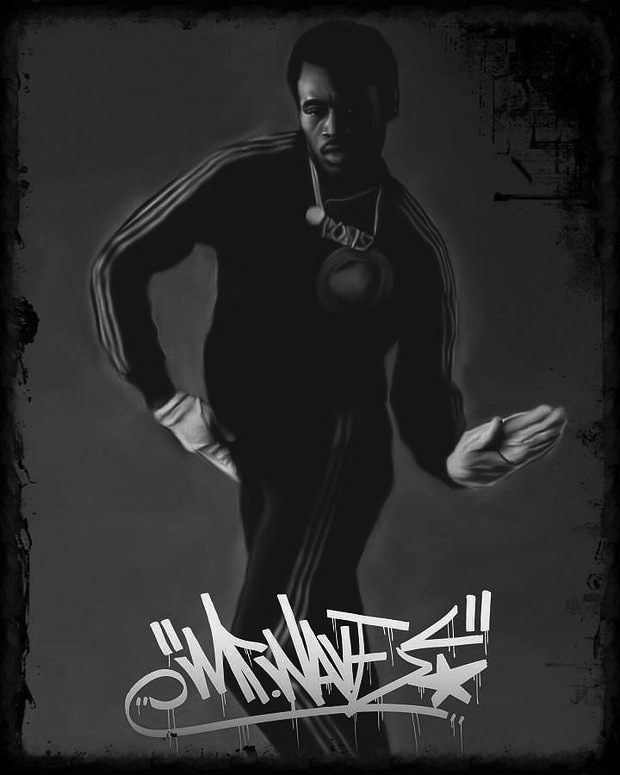
\includegraphics[width=\linewidth]{mr_wave.jpg}
  \caption{Portrait of Mr. Wave}
  \label{fig:marginfig}
\end{marginfigure}

\marginnote[30pt]{Mr. Wave (AKA Tony Draughon) was an original member of New York City Breakers.  As an actor he was best known for his performance in the film classic \textit{Beat Street} (1984).  \\ \ \\ \ \\ \ \\
Waving is an illusionary dance style composed of a series of movements that give the appearance that a wave is traversing through a dancer's body.  Waving is thought to have grown out of the popping and funk dance scene.}

\begin{marginfigure}[60pt]
  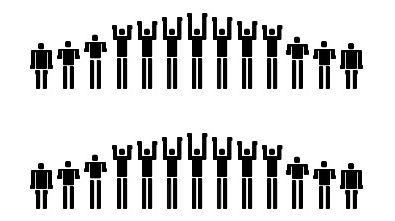
\includegraphics[width=\linewidth]{the_wave.jpg}
  \caption{Diagram of "The Wave"}
  \label{fig:marginfig}
\end{marginfigure}

\section{Media and Disturbance}
\newthought{A wave is a disturbance}, or oscillation, which propagates through space.  It delivers energy, or information, from one point to another.  We begin to theorize waves considering three criteria for their existence.
\begin{itemize}
\item \textbf{source}\\ A disturbance originates from some region of space at some time.
\item \textbf{medium}\\ The disturbance must propagate through some medium. 
\item \textbf{interaction}\\  For the disturbance to propagate through space there must be some physical means by which adjacent portions of the medium interact in order to pass the disturbance through space.
\end{itemize}
This being said, we may imagine a universe where "in the beginning" waves exist and need not a source.  In addition, the vacuum of empty space may provide the medium for energy to propagate.  A medium is typically considered to be an assembly, or continuum, of "stuff" with inertial properties.  Waves may also travel through nothing. 

\section{Wave Types}

\begin{description}
  \item[transverse wave] A propagating wave that causes the particles of the disturbed medium to move \textbf{perpendicular} to the direction of wave propagation.  "The Wave" at sporting events travels through the crowd as a transverse wave.  
  \item[longitudinal wave] A propagating wave that causes the particles of the disturbed medium to move \textbf{parallel} to the direction of wave propagation.  Sound travels through air as a longitudinal wave.
  
\end{description}

\begin{marginfigure}[0pt]
  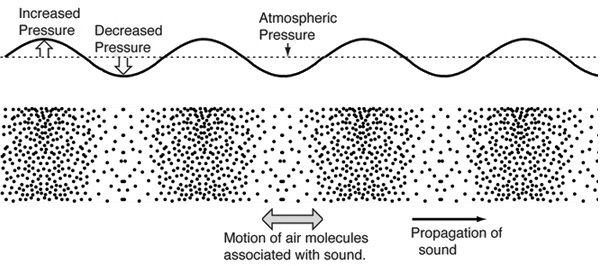
\includegraphics[width=\linewidth]{lwav.jpg}
  \caption{Longitudinal wave}
  \label{fig:marginfig}
\end{marginfigure}

\section {One Dimensional Waves}
A wave can take many forms.  In one dimension a wave can be represented by any function of the position plus/minus the product of velocity and time.  The amplitude $A$ represents the maximum value of the function $f(x \pm vt)$.  The wave velocity is the time rate of change of the position on some point of the function $f(x)$.
$$y=f(x-vt) \hspace{2cm} \text{propagation in positive direction}$$
$$y=f(x+vt) \hspace{2cm} \text{propagation in negative direction}$$
$$A=f_{max}$$
$$v=\lim _{\Delta \rightarrow 0}\frac{\Delta x}{\Delta t}=\frac{dx}{dt}=-\frac{\frac{\partial f}{\partial t}}{\frac{\partial f}{\partial x}}$$

\begin{marginfigure}[-130pt]%
\begin{tikzpicture}
    [line cap=round,line join=round,x=2cm,y=2cm, scale=1.2, decoration={brace,amplitude=2pt}]
 \draw[smooth,samples=100,domain=0:2]
                                 plot(\x,{1.5/(sqrt(2*pi))*exp(-((\x-0.5)^2)/(2*0.1^2))});
 \draw[smooth,samples=100,domain=0:2]
                                 plot(\x,{1.5/(sqrt(2*pi))*exp(-((\x-1.5)^2)/(2*0.1^2))});
   \draw[-latex,color=black,thin] (-0.2,0) -- (2,0) node [anchor=north ,scale=1] {$x$};
   \draw[-latex,color=black,thin] (0,-0.2) -- (0,1.4)node [anchor=east ,scale=1] {$y$};
   \draw (0.7,1) node [anchor=south west ,scale=1] {$f(x-vt)$};
      \draw (0.5,0.6) node [anchor=south ,scale=1] {$t=1$};
   \draw (1.5,0.6) node [anchor=south ,scale=1] {$t=2$};
 \end{tikzpicture}
  \caption{A wave pulse traveling in the positive $x$ direction}
  \label{fig:marginfig}
\end{marginfigure}
 
 \section{Supersposition}
 If two waves are simultaneously propagating through a medium the resultant wave function at any point is the algebraic sum of the wave wave functions of the individual waves.
 
 \section{Waves on Strings (Transverse)}
 \newthought{Consider a wave pulse} traveling along a string with tension $T$ and linear mass density $\mu$.  Zooming in closely to a section of the string the curvature is constant and can therefore be approximated by a circular arc of radius $R$ and angle $\theta$.  \\
The section of string has a net force $F_r$ on it which restores it to equilibrium and a mass $m$.
$$F_r=2F\sin\theta\approx 2F\theta$$
$$m=\mu \Delta s= 2\mu R \theta$$
This force accelerates the section of string centripetally so the velocity of the section of string may be determined as follows.
$$F_r=\frac{mv^2}{R} \hspace{1cm} \longrightarrow \hspace{1cm} 2F\theta=\frac{2\mu R \theta v^2}{R}$$
$$v=\sqrt{\frac{F}{\mu}}$$

\begin{marginfigure}[-220pt]
  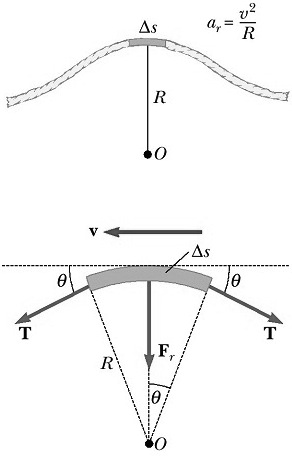
\includegraphics[width=\linewidth]{string_wave.jpg}
  \caption{Transverse wave on a string}
  \label{fig:marginfig}
\end{marginfigure}

 \section{Reflection at an Interface}
 
 \begin{itemize}
\item When a wave meets a free boundary, or travels to a less dense/lower velocity medium,  the reflected pulse is not inverted.
\item When a wave meets a fixed boundary, or travels to a more dense/higher velocity medium, the reflected pulse is inverted. 
\end{itemize}

\begin{marginfigure}[0pt]
  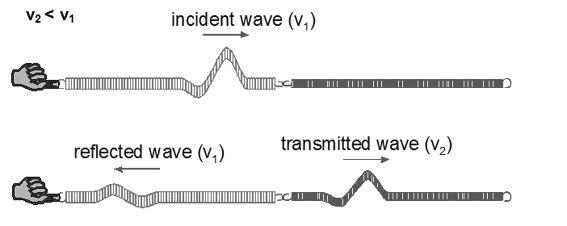
\includegraphics[width=\linewidth]{wave_interface.jpg}
  \caption{Transverse wave at an interface (no inversion)}
  \label{fig:marginfig}
\end{marginfigure}

\begin{marginfigure}[0pt]
  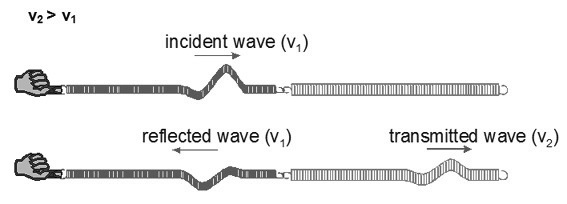
\includegraphics[width=\linewidth]{wave_interface2.jpg}
  \caption{Transverse wave at an interface (inversion)}
  \label{fig:marginfig}
\end{marginfigure}

\section{Sinusoidal Waves}
A sinusoidal wave is the smoothest periodic wave.  Here $y$ represents the displacement from equilibrium.  It can represent pressure or a spatial dimension.  $A$ is the amplitude.  It is the maximum $y$ value.  $x$ is the spatial dimension in the direction of propagation.  $t$ is time.  $\phi$ is the phase.  $k$ and $\omega$ are the coefficients of $x$ and $t$ respectively.  
$$y=A\cos\left( kx - \omega t+\phi\right)$$
$k$ and $\omega$ determine the spatial and temporal periodicity.  $\lambda$ is the wavelength and $T$ is referred to as the period.  The wave length is the distance between identical points in the wave.  The period is the time between wave cycles.
$$k\lambda=2\pi \hspace{2cm} \omega T=2\pi$$
The wave speed is defined as the ratio of the wavelength and the period.  It is the speed at which some point on the pattern travels.  It does not represent the speed of any particles in the medium.
$$v_{wave}=\frac{\lambda}{T}=\frac{\omega}{k}$$

\begin{figure}
  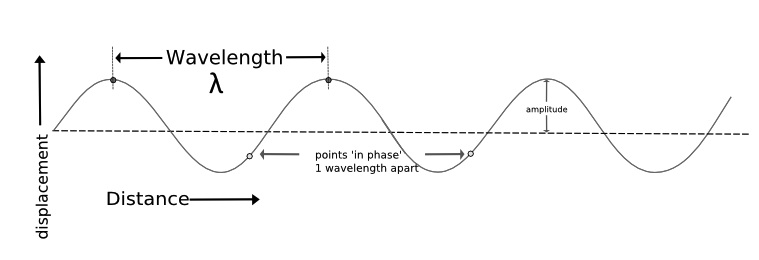
\includegraphics[width=\linewidth]{sine_wave.jpg}
  \caption{Sine wave }
  \label{fig:marginfig}
\end{figure}

\subsection{Power}
\marginnote{The power delivered by the wave can be thought of as the rate kinetic energy is delivered in the medium. }
$$\Delta E=\frac{1}{2}(\Delta m)\omega^2A^2=\frac{1}{2}(\mu \Delta x)\omega^2A^2$$
$$P=\frac{\Delta E}{\Delta t}=\frac{1}{2}\mu\omega^2A^2 \frac{\Delta x}{\Delta t}=\frac{1}{2}\mu\omega^2A^2 v_{wave}$$

\newpage

\section{Wave Equation}
Given a scalar function $u(\overrightarrow{\scriptr})$, such as pressure, and propagation speed $c$ we have the following differential equation.  This is known as the wave equation. 
$${\partial^2 u \over \partial t^2} = c^2 \nabla^2 u$$
The functions which obey this differential relationship are waves.  When this differential equation arrises in the analysis of some system it means the systems supports the propagation of waves.

\marginnote{The speed of sound varies with temperature, pressure and the density of the material.  The speed of sound (m/s) in air (at 1 atm) varies with temperature (Celsius) as follows.
$$v=331+0.6T$$}
\section{Sound Waves}
Sound is defined by ANSI as "Oscillation in pressure, stress, particle displacement, particle velocity, etc., propagated in a medium with internal forces (elastic or viscous)."  It can propagate through compressible media such as air, water and solids as longitudinal waves or transverse waves in solids. 
\marginnote{Humans can hear sounds in the range of 20 to 20,000 Hertz, though there is variation between individuals.  Elephants can hear sounds at 14-16hz, while some whales can hear subsonic sounds as low as 7hz (in water).}


The velocity of sound in a medium depends its elastic and inertial properties.
$$v=\sqrt{\frac{\text{elastic property}}{\text{inertial property}}}=\sqrt{\frac{B}{\rho}}$$
\subsection{Power, Intensity and Sound Level}
Consider a sound source emitting energy at a rate $P$.  This is the power of the source.  The intensity of the sound, captured by some observer, is the power per unit area.
$$I=\frac{\text{Power}}{\text{Area}}$$
\begin{marginfigure}[0pt]
  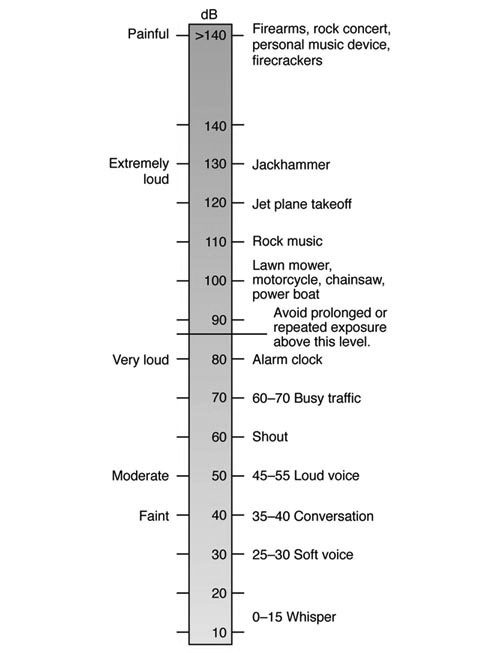
\includegraphics[width=\linewidth]{decibel.jpeg}
  \caption{The decibel scale}
  \label{fig:marginfig}
\end{marginfigure}
The decibel scale of intensity is a logarithmic scale.  The reference value $I_0$ is the lowest intensity of audible sound.
$$\beta=10\  \log \frac{I}{I_0} \hspace{2cm} I_0=10^{-12} \ W/m^2$$

\subsubsection{Spherical, Cylindrical and Linear Waves}
Spherically symmetric waves disperse power over the the surface of a sphere.  Cylindrically symmetric waves disperse power over the the surface of a cylinder.
$$I_{sphere}=\frac{P}{4\pi r^2} \hspace{2cm} I_{cyl}=\frac{P}{2\pi r}$$
Symmetric waves in one dimension give the following intensity.
$$I=\frac{P}{2}$$


\subsection{Doppler Effect}
The Doppler effect is the change in frequency of a wave for an observer moving relative to its source. It is named after the Austrian physicist Christian Doppler, who proposed it in 1842 in Prague. It is commonly heard when a vehicle sounding a siren or horn approaches, passes, and recedes from an observer. Compared to the emitted frequency, the received frequency is higher during the approach, identical at the instant of passing by, and lower during the recession.

$$f = \left ( \frac {c+v_\text{reciever}}{c + v_\text{source}} \right ) f_0$$
\subsection{Standing Waves \& Resonance}
A standing wave is associated with each point on the axis of the wave having an associated constant amplitude. The locations at which the amplitude is minimum are called nodes, and the locations where the amplitude is maximum are called antinodes.

It arises as a result of interference between two waves traveling in opposite directions.  Resonance is the manifestation of standing waves inside a resonator due to interference between waves reflected back and forth at the resonant frequency.
\marginnote{
$$\cos{a}+\cos{b}=2\cos\frac{a+b}{2}\cos\frac{a-b}{2}$$ 
\\ \ \\
$$\sin{a}\pm\sin{b}=2\sin\frac{a\pm b}{2}\cos\frac{a\mp b}{2}$$}

$$A_0\cos(kx-\omega t)+A_0\cos(kx+\omega t)=2A_0 \cos(kx)\cos(\omega t)$$

\subsection{Beats}
A beat is an interference pattern between two sounds of slightly different frequencies, perceived as a periodic variation in volume whose rate is the difference of the two frequencies.  When tuning instruments that can produce sustained tones, beats can readily be recognized. 
$$A_0\cos(\omega_1 t)+A_0\cos(\omega_2 t)=2A_0 \cos(\frac{\omega_1-\omega_2}{2}t)\cos(\frac{\omega_1+\omega_2}{2}t)$$
\chapter{Electrostatics}

\textit{We call that fire of the black thunder-cloud 'electricity,' and lecture learnedly about it... but what is it?}\\
\noindent\textbf{-   Thomas Carlyle}

\vspace{1cm}


\begin{marginfigure}%
  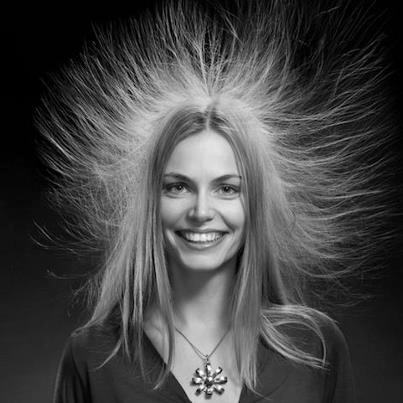
\includegraphics[width=\linewidth]{hair_static.jpg}
  \caption{Amber and her charged hair}
  \label{fig:marginfig}
\end{marginfigure}

\marginnote{In the colder months, when the air has less moisture, hair picks up electrical charge.  Fight this unfortunate situation by switching to a more hydrating shampoo and conditioner.}

\section{Background}
Electrostatics deals with the phenomena and properties of stationary charges.   The ancients knew materials such as amber attract lightweight particles after rubbing.   Thales of Miletus made a series of observations on static electricity around 600 BC.  The word electricity comes from the Greek word for amber.  Electrostatic phenomena arise from the forces that electric charges exert on each other.
\begin{itemize}
\item there are two kinds of charge in nature of which opposite attract and like repel
\item charge is conserved
\item charge is quantized
\end{itemize}

\section {Coulomb's Law}

\begin{marginfigure}%
  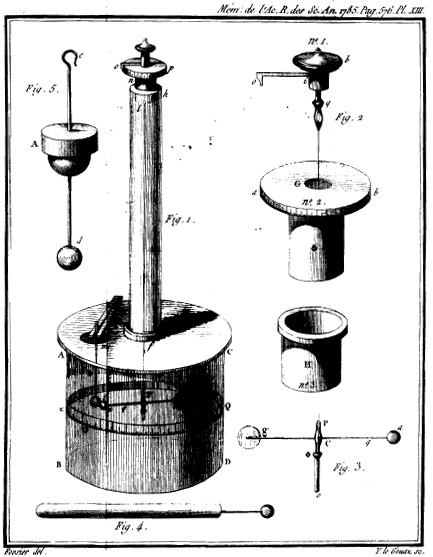
\includegraphics[width=\linewidth]{torsion.jpg}
  \caption{Coulomb's torsion balance}
  \label{fig:marginfig}
\end{marginfigure}

Coulomb's law describes the electrostatic interaction between electrically charged particles. The law was first published in 1784 by French physicist Charles Augustin de Coulomb. It is analogous to Isaac Newton's inverse-square law of universal gravitation.

$$F_{E}=k_e\frac{q_1q_2}{r^2}$$
$$\overrightarrow{F}_{2\rightarrow 1}=-k_e\frac{q_1q_2}{r^2} \hat{r} \hspace{2cm} \overrightarrow{r}=\overrightarrow{r}_2-\overrightarrow{r}_1$$


$$\begin{tikzpicture}[scale=1]
     	
	\fill[black] (-6,0) circle (0.5mm) node [anchor=west ,scale=1] {$F_E$};   
	\draw[->,thick] (-6,0) -- (-7,0) ; 
	\fill[black] (6,0) circle (0.5mm) node [anchor=east,scale=1] {$F_E$};   
	\draw[->,thick] (6,0) -- (7,0) ; 
	 \draw[very thick] (-4,0) circle (0.5cm) node {$q_1$};
	  \draw[very thick] (4,0) circle (0.5cm) node {$q_2$};
	    \draw[thick, color=gray,->] (-4,-0.75) --   (4,-0.75) node [midway, anchor=south] {$\overrightarrow{r}$};
	     
	     
	       \begin{scope}[shift={(-3,0)}, scale=0.75] 
	 
	   \draw[thick](0.2,0.1) -- (0.2,-0.1);
	    \draw[ thick,-stealth] (0.1,0) -- (1,0) node [near start,anchor=north]{\scriptsize $r$};  
	  \end{scope}	     
   \end{tikzpicture}$$


\newpage

\section{Constants}

\begin{table}[h]\index{typefaces!sizes}
  \footnotesize%
  \begin{center}
    \begin{tabular}{lcl}
      \toprule
     Constant & Variable & Quantity \\
      \midrule
 Electrostatic Constant   & $k_e$           & $8.9875 \times 10^{9}\  \nicefrac{ \text{N}\cdot\text{m}^2}{\text{C}^2}$    \\
    Fundamental Charge       & $e$             & $1.6022 \times 10^{-19}\  \text{C}$                                          \\
    Mass of the Electron     & $m_e$           & $9.1095 \times 10^{-31}\  \text{kg}$                                         \\
    Mass of Proton           & $m_p$           & $1.6726 \times 10^{-27} \ \text{kg}$                                         \\ 
    Mass of Neutron           & $m_n$           & $1.6749 \times 10^{-27}\  \text{kg}$                                         \\ 
    Vacuum Permativity       & $\epsilon_0$ & $8.8542 \times 10^{-12}\  \nicefrac{ \text{F}}{\text{m}}$                    \\ 
    Speed of Light       & $c$ & $2.998 \times 10^{8}\  \nicefrac{ \text{m}}{\text{s}}$                    \\ 
      \bottomrule
    \end{tabular}
  \end{center}
  \caption{Physical constants for electrostatics}
  \label{tab:font-sizes}
\end{table}

\marginnote[-50pt]{
$$ k_e=\frac{1}{4\pi \epsilon_0}$$}


\marginnote[0pt]{
The unit of electric charge is the Coulomb, denoted C.}

\section {Electric Field}
The concept of an electric field, or E-field, was introduced by Michael Faraday.  The electric field $\overrightarrow{E}(\overrightarrow{r})$ is a vector field, meaning it is a vector quantity at every point in space.  At a single point in space, the electric field represents the force that would be exerted on a one Coulomb "test charge".  The E-field is the electrostatic force per unit charge.
$$\overrightarrow{E}=\frac{\overrightarrow{F}_e}{q_0}$$
There is an electric field surrounding every charge distribution.  Consider the E-field to represent a feature of space that represents the possibility of electric force, if there were a charge there.
\subsection{Point Charge}
Consider a point charge located at point $\overrightarrow{b}$.  The electric field at a location $\overrightarrow{r}$, due to the presence of the  point charge is represented as follows.  
$$\overrightarrow{E}(\overrightarrow{r})=k_e\frac{q}{R^2}\hat{R} \hspace{1cm} \overrightarrow{R}=\overrightarrow{r}-\overrightarrow{b}$$
A point charge located at the origin of coordinates will generate the following electric field
$$\overrightarrow{E}(\overrightarrow{r})=k_e\frac{q}{r^2} \hat{r} $$

\marginnote[-300pt]{
\subsection{Superposition}
The principle of superposition applied to electrostatic distributions means the force on a given charge $Q$ is the vector sum of forces from interactions with a set of charges.  
$$\overrightarrow{F}_E=k_e\sum_{i=1}^{N} \frac{Qq_i}{R_i^2} \hat{R}_i $$
Equivalently the electric field at a given point in space is the vector sum of the fields due to the set of charges around it.
$$\overrightarrow{E}(\overrightarrow{r})=k_e\sum_{i=1}^{N} \frac{q_i}{R_i^2} \hat{R}_i $$
}


\begin{marginfigure}[-60pt]%
  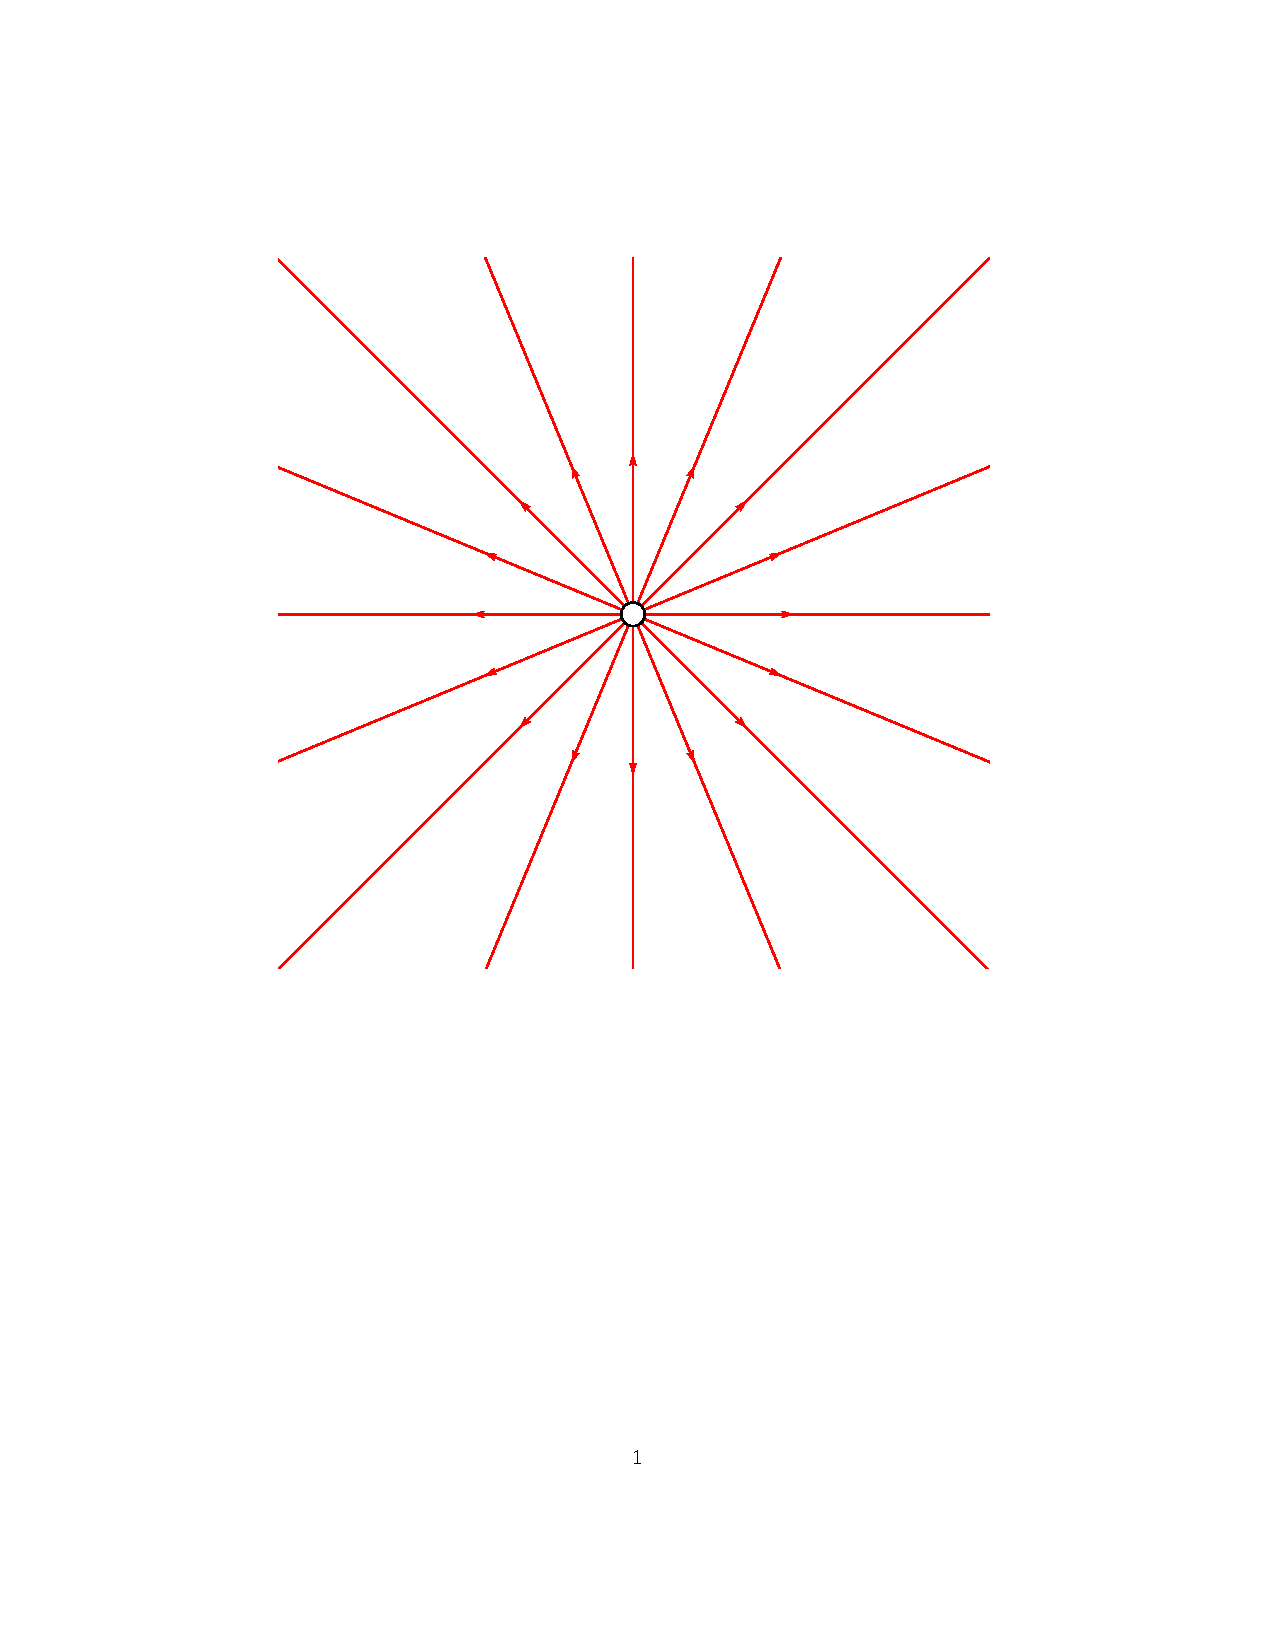
\includegraphics[width=\linewidth ,trim={7cm 14cm 7cm 7cm},clip]{monopole_graph.pdf}
  \caption{Single positive charge}
  \label{fig:marginfig}
\end{marginfigure}




  \section{Electric Field Lines}
  Electric field lines are a visual tool used to visualize the strength and direction of the electric field in space.  While they are not real, per se, they provide an extremely useful representation for the permeation of electric field through space.  
  \begin{itemize}
 \item Electric field lines emanate perpendicularly out of positive charge and sink perpendicularly into negative charge.  They may also terminate/emanate at infinity if the net charge of the distribution is non-zero.
 \item The number of field lines drawn entering/exiting a charge is proportional to the amount (magnitude) of charge.
 \item  The electric field vector is directed tangent to the field line at each point in space.
 \item No two field lines can cross
 \item  The number of lines per unit area is proportional to the field strength in that area.  Thus $E$ is strong when field lines are close together while $E$ is weak when field lines are far apart.
 \
 \end{itemize}


\begin{marginfigure}[-250pt]%
  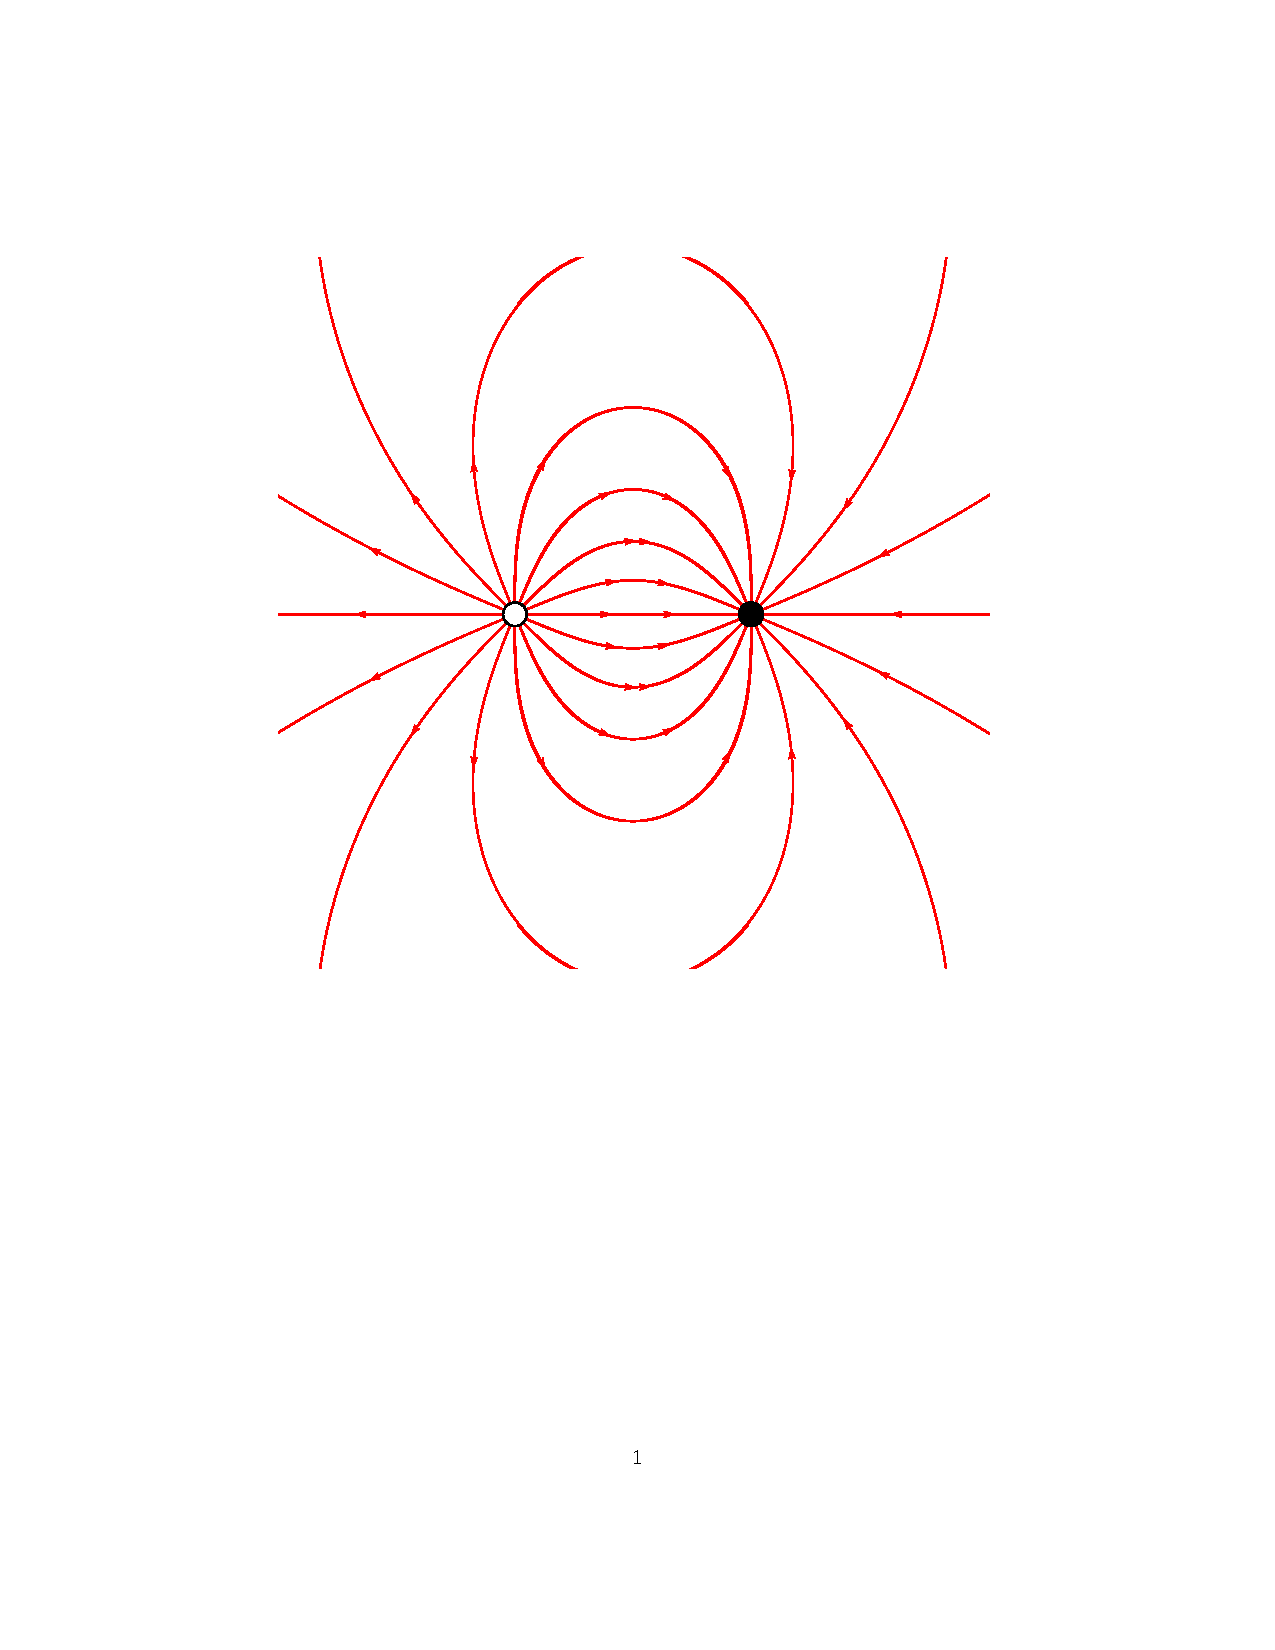
\includegraphics[width=\linewidth ,trim={7cm 14cm 7cm 7cm},clip]{dipole_graph.pdf}
  \caption{Dipole field close up}
  \label{fig:marginfig}
\end{marginfigure}

\begin{marginfigure}[-40pt]%
  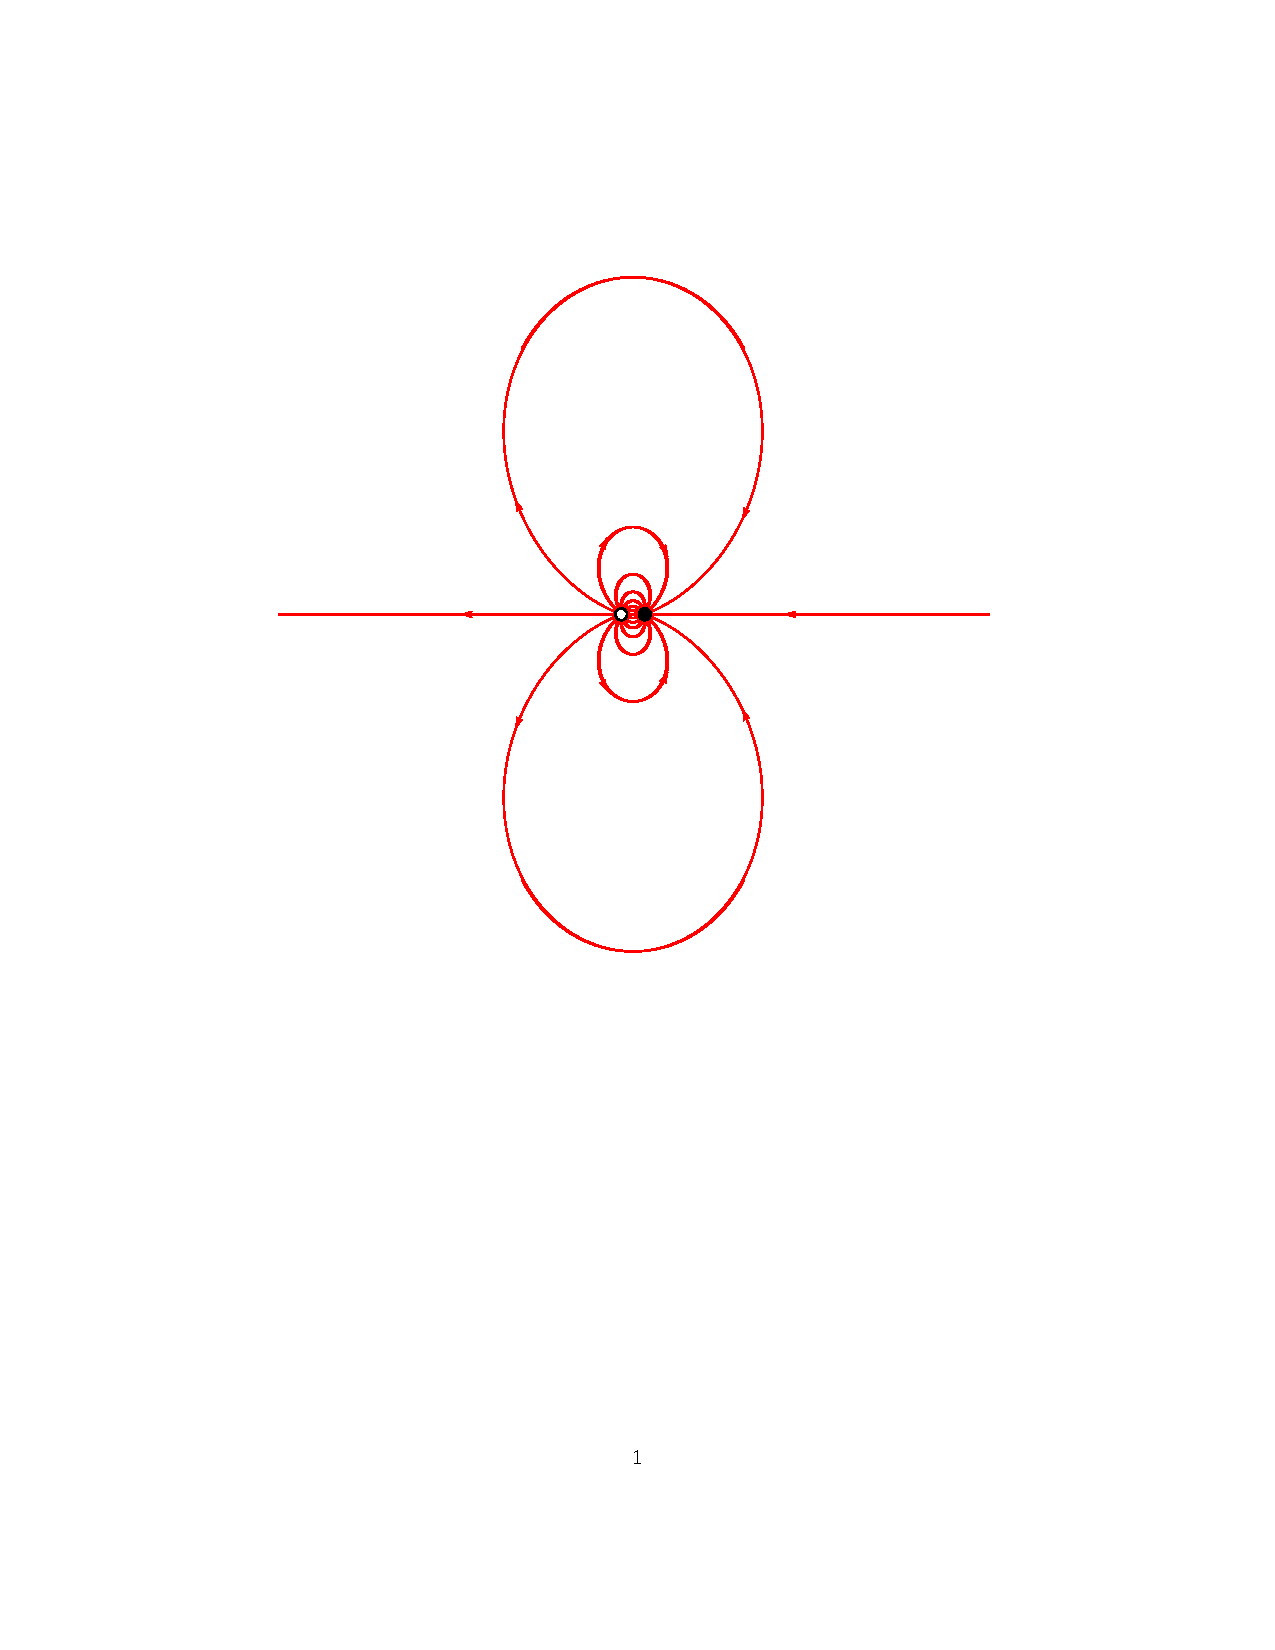
\includegraphics[width=\linewidth ,trim={7cm 15cm 7cm 8cm},clip]{dipole_far2.pdf}
  \caption{Dipole field far away}
  \label{fig:marginfig}
\end{marginfigure}

\begin{marginfigure}[10pt]%
  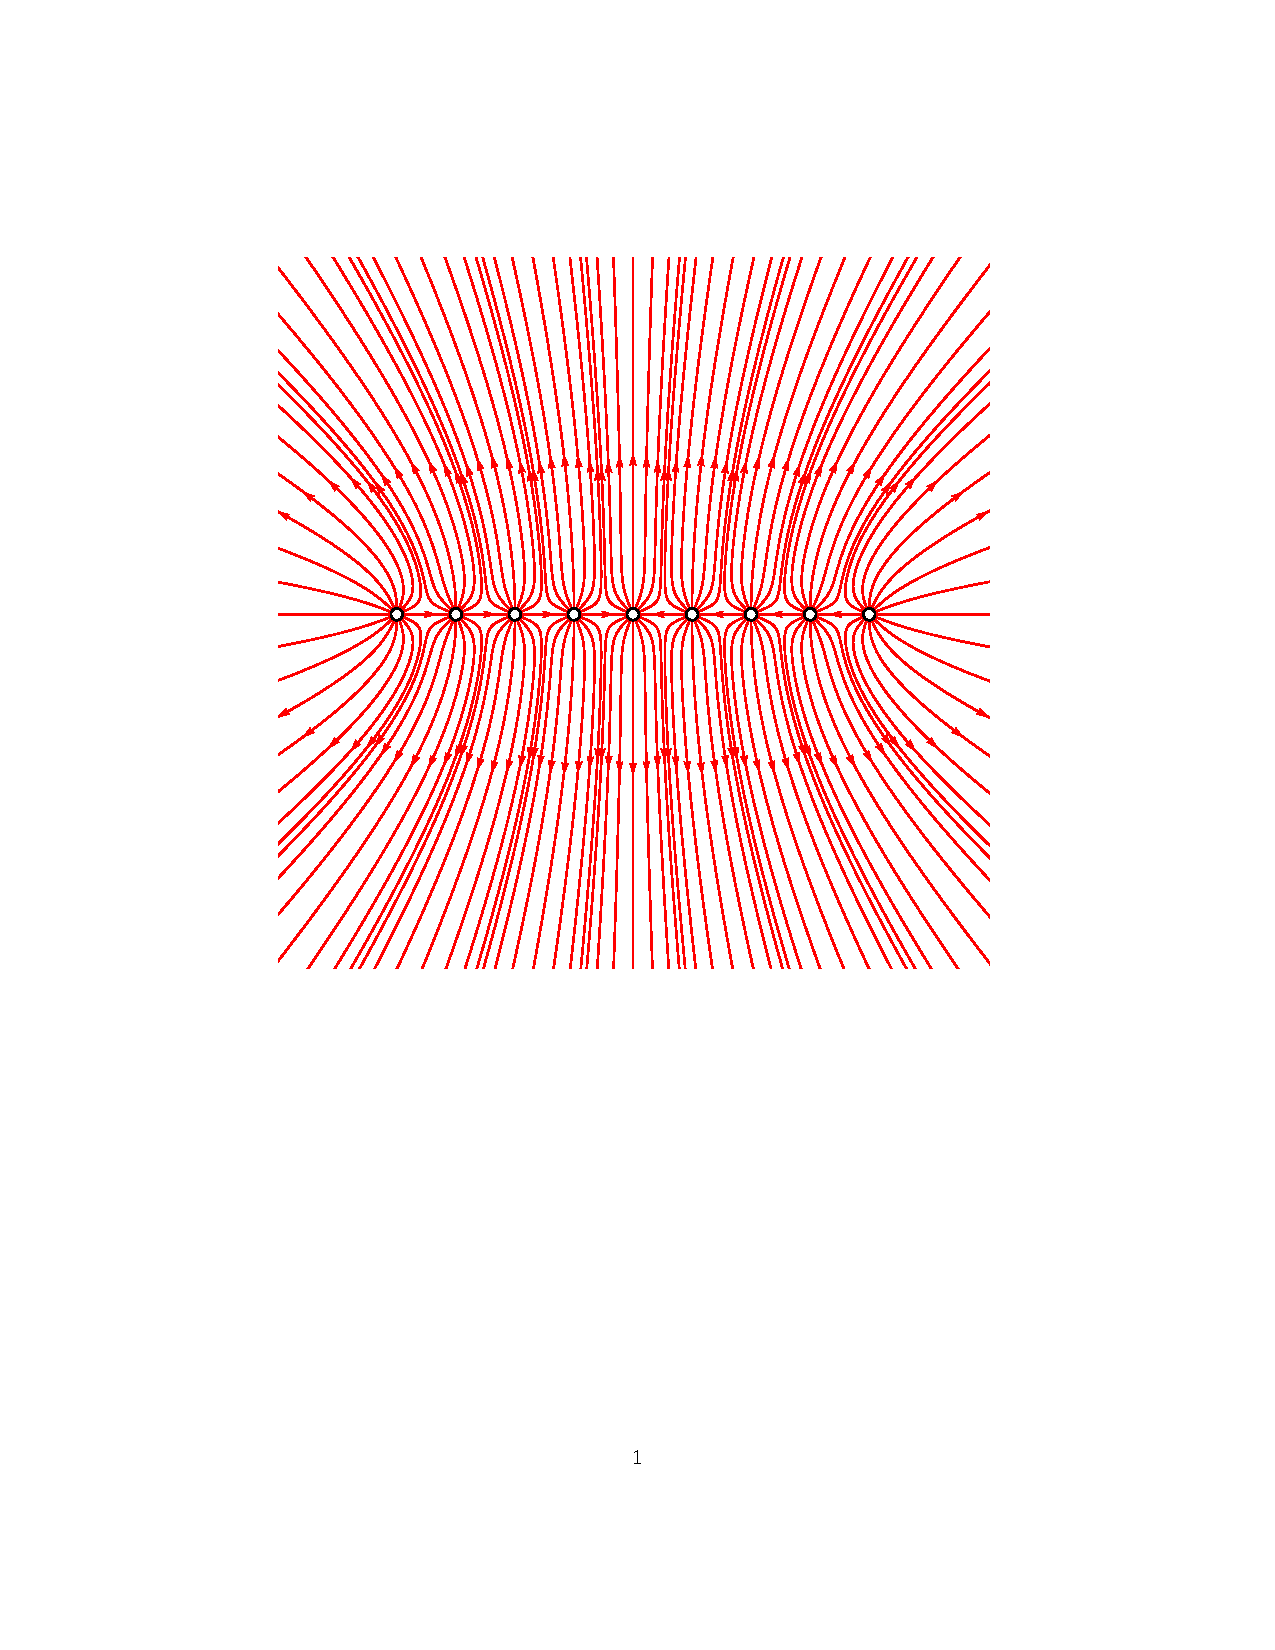
\includegraphics[width=\linewidth ,trim={6cm 14cm 6cm 7cm},clip]{Efield_graph2.pdf}
  \caption{Superposition of multiple positive point charges in a row}
  \label{fig:marginfig}
\end{marginfigure}

\begin{marginfigure}[0pt]%
  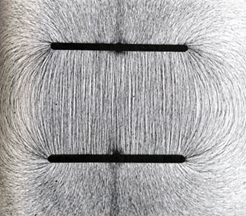
\includegraphics[width=\linewidth]{electric_fields.jpg}
  \caption{Electric field between two charged plates}
  \label{fig:marginfig}
\end{marginfigure}

%\subsection{Continuous Distribution}
%$$\overrightarrow{E}=k_e\int \frac{dq}{r^2} \hat{r} $$

 
 \section{Charge Distributions}
 A charge distribution is any arrangement of charge in space.  It may consist of a set of various point charges at different locations in space or be a continuous distribution of charge.  Continuous charge distributions may be represented by charge per unit volume, charge per unit area, or charge per unit distance.  These are  types of charge density. 
 $$\text{Volume density} \hspace{2cm} \rho=\frac{Q}{V}$$
  $$\text{Surface density} \hspace{2cm} \sigma=\frac{Q}{A}$$
   $$\text{Line density} \hspace{2cm} \lambda=\frac{Q}{L}$$
   
 \section{Types of Materials}
Atomic lattices making up bulk materials have different electron energy levels or bands.  \textbf{Valence bands} are associated with individual atomic orbital.  Their electrons are spatially localized and lower energy.   \textbf{Conduction bands} are associated with delocalized or free electrons able to move throughout the bulk material.  The energy difference between the highest valence band and lowest conduction band is known as the \textbf{band gap}.  Electrons fill lowest first.  The \textbf{Fermi level} is a thermodynamic property that corresponds to the hypothetical energy of an electron added to the system.  
   
 \newpage  
   
 \begin{description}
  \item[Conductors] In conductors the Fermi level is in conduction band.  This means electrons added to the system are not spatially isolated and is free to move around.  This so called "free charge" accumulates on the surface of the bulk material and congregates more densely in kinks and furrows.
  \item[Insulators]  For insulators the Fermi level in a large band gap.  There are no free electrons.  They are bound locally.  Charge is not free to move around.
   \item[Semiconductors]  In semiconductors the band gap is small so electrons can be easily bumped from localized states to delocalized states in conduction bands.
\end{description}
  
   
   \begin{marginfigure}[-180pt]%
  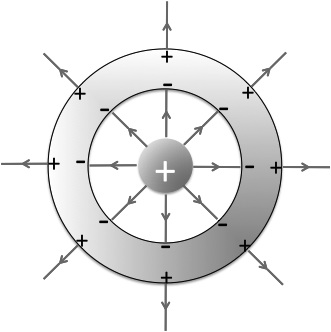
\includegraphics[width=\linewidth]{conductor.jpg}
  \caption{Electric field and charge distribution in a conducting sphere}
  \label{fig:marginfig}
\end{marginfigure}

\begin{marginfigure}[40pt]%
  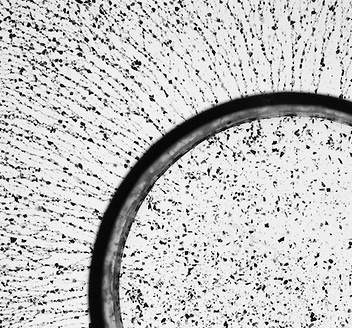
\includegraphics[width=\linewidth]{conductor2.jpg}
  \caption{Electric field inside and outside a conducting sphere}
  \label{fig:marginfig}
\end{marginfigure}
   
 \section{Field and Charge Distributions in Conductors}
 \begin{itemize}
 \item The electric field is zero everywhere inside the conductor.
 \item  Any charge on an isolated conductor resides on its surface.
 \item  The electric field just outside a charged conductor is perpendicular to the surface and has a magnitude of $\frac{\sigma}{2\epsilon_0}$.
 \item On an irregularly shaped conductor, charge tends to accumulate at locations where the radius of curvature is smallest such as edges, corners and points.
 \end{itemize}
 

\begin{marginfigure}[80pt]%
  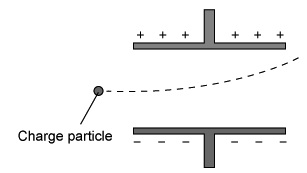
\includegraphics[width=\linewidth]{charge_particle.jpg}
  \caption{Motion of charged particle between two charged plates}
  \label{fig:marginfig}
\end{marginfigure}

 \section{Motion of a Charged Particle}
 Electromagnetic forces are similar to gravity in their relationship to space but are extremely different in one respect.  In gravity mass is responsible for gravitational force but also provides inertia.  For charged particles charge is the source of the electrostatic force but mass still provides the inertia.  
 $$\overrightarrow{F}_{net}=m\overrightarrow{a}$$
 $$\overrightarrow{F}_{net}=q\overrightarrow{E} \hspace{1cm} \longrightarrow \hspace{1cm} \overrightarrow{a}=\frac{q}{m}\overrightarrow{E}$$
 If we generate a field in space and drop a particle in that field then the charge-to-mass ratio can be known through measuring the acceleration.

\newpage

\begin{marginfigure}[50pt]%
  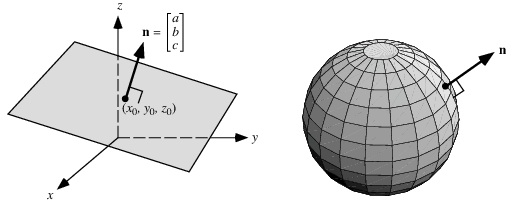
\includegraphics[width=\linewidth]{normal.jpg}
  \caption{Surface normal vector}
  \label{fig:marginfig}
\end{marginfigure}

\begin{marginfigure}[0pt]%
  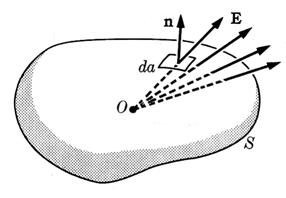
\includegraphics[width=\linewidth]{gauss_law.jpg}
  \caption{Schematic of Gauss's law }
  \label{fig:marginfig}
\end{marginfigure}

  \section{Electric Flux}
  Electric flux, $\Phi_E$, is the measure electric field passing through a given surface area. Electric flux is proportional to the number of electric field lines perforating the surface.  
  \subsection{Uniform Field Through a Flat Surface}
  For a flat surface and constant field it is the dot product of the electric field vector and the vector normal to the surface.  A surface normal vector points straight out of a surface.
  $$\Phi_E=EA\cos\theta=\overrightarrow{E}\cdot \overrightarrow{A}$$  
  \subsection{Variable Field Through a Set of Flat Surfaces}
  For a variable field through a set of flat surfaces simply take the sum of the flux through all of the surfaces.
  $$\Phi_E=\sum_{i=1}^{N} \overrightarrow{E}_i\cdot \overrightarrow{A}_i$$
   \subsection{Variable Field Through a Continuous Surface}
   A variable field through a continuous smoothly curved surface is modeled as the limit of area elements going to zero. 
   $$\Phi_E=\lim_{\Delta A \rightarrow 0 }\sum_{i=1}^{N} \overrightarrow{E}_i\cdot \Delta \overrightarrow{A}_i$$
   
   \marginnote[-100pt]{
    $$\lim_{\Delta A \rightarrow 0 }\sum_{i=1}^{N} \overrightarrow{E}_i\cdot \Delta \overrightarrow{A}_i=\lim_{\Delta V \rightarrow 0 }\sum_{j=1}^{M} \nabla \cdot \overrightarrow{E}_i\Delta {V}_i$$
}

 \marginnote[-50pt]{
    $$q_{enc}=\lim_{\Delta V \rightarrow 0 }\sum_{j=1}^{M} {\rho}_i\Delta {V}_i$$
}

   \marginnote{
    $$ \nabla \cdot \overrightarrow{E}_i=\frac{ {\rho}_i}{\epsilon_0}$$
}
     \section{Gauss's Law}
     Gauss's law states the total of the electric flux out of a closed surface is equal to the charge enclosed divided by the permittivity.
    \subsection{Variable Field Through a Continuous Closed Surface}
    $$\Phi_E=\lim_{\Delta A \rightarrow 0 }\sum_{i=1}^{N} \overrightarrow{E}_i\cdot \Delta \overrightarrow{A}_i=\frac{q_{inc}}{\epsilon_0}$$
     \subsection{Uniformly Normal Field of Constant Magnitude Through a Continuous Closed Surface}
     $$\Phi_E=EA=\frac{q_{inc}}{\epsilon_0}$$
     
 

 \begin{marginfigure}[-100pt]%
 $$ 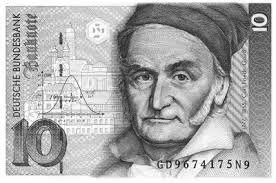
\includegraphics[width=\linewidth]{gauss_money.jpeg}$$
  \caption{Gauss on money }
  \label{fig:marginfig}
\end{marginfigure}

    \newpage

  \section{Work and Electrostatic Potential Energy}
   
  \marginnote[0pt]{The potential energy $U$ is undetermined up to a constant.  The real physically measurable quantity is the change in potential energy, $\Delta U$.}
  
  \marginnote[10pt]{An individual particle does not have potential energy, $U$ resides in the field (if anywhere) and "belongs" to the system as a whole.  If two charged particles are in proximity they do not each have a potential energy.  There is one electrostatic potential energy between the two particles.}
  
  \marginnote[10pt]{Potential energy is only a meaningful concept for certain types of forces, namely conservative forces.  Remember, the total work done on a particle moving from point $A$ to point $B$ must be independent of path for conservative forces.  }
  
  Electrostatic potential energy, $U$, that results from Coulomb forces and is associated with the configuration of a particular set of point charges within a defined system.  An object contributes to the electrostatic potential energy of a system due to its own electric charge and its relative position to other electrically charged objects.
 
  Recall the definition for change in potential energy and the definition of work.
  $$\Delta U=-W \hspace{1cm} W= \sum_A^B \overrightarrow{F}\cdot \Delta\overrightarrow{s}$$
  Combining the above, and expressing the force in terms of the field, yields the following equation.
  $$\Delta U =- q_0 \sum_A^B \overrightarrow{E}\cdot \Delta\overrightarrow{s}$$
  Consider path-summation on the right hand side of the equation.  Note it is purely a function space, the field in the space and the path.  It is independent of the charge.  In addition, since the electrostatic force is conservative, this path-summation is path-independent.   Therefore it only depends on the endpoints of the path and not the path itself.
  
  \section{Electric Potential}
   \marginnote[0pt]{$$\text{Volt}\equiv\frac{\text{Joule}}{\text{Coulomb}}$$}
    \marginnote[0pt]{ }
  We name the field path-summation $\Delta V$, the change in electric potential.
  $$\Delta V=-\sum_A^B \overrightarrow{E}\cdot \Delta \overrightarrow{s}$$
  $\Delta V$ can be considered the change in electrostatic potential energy per unit charge.
  $$\Delta V=\frac{\Delta U}{q_0}$$
  Finally, after choosing a zero reference, we can write the equation representing the voltage (electric potential) as the electric potential energy per unit charge.
  $$V(\overrightarrow{r})=\frac{U(\overrightarrow{r})}{q_0}$$
   \begin{marginfigure}[0pt]%
 $$ 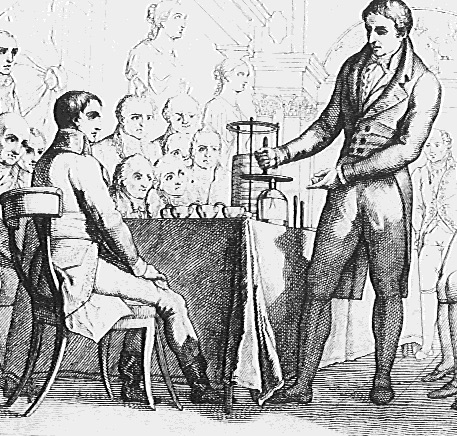
\includegraphics[width=\linewidth]{volt.jpg}$$
  \caption{Alessandro Giuseppe Antonio Anastasio Volta showing his experiments in electricity to Napolean Bonaparte}
  \label{fig:marginfig}
\end{marginfigure}
  The electric potential is a scalar field.  Like the electric field, it is a feature of space independent of the charge we put in the space.  While the electric field represents a vector quantity at every point in space, the voltage (electric potential) represents a single value quantity (scalar quantity) at every point in space.
  
  \newpage
  
  \subsection{Uniform Field}
  \begin{marginfigure}[-10pt]%
  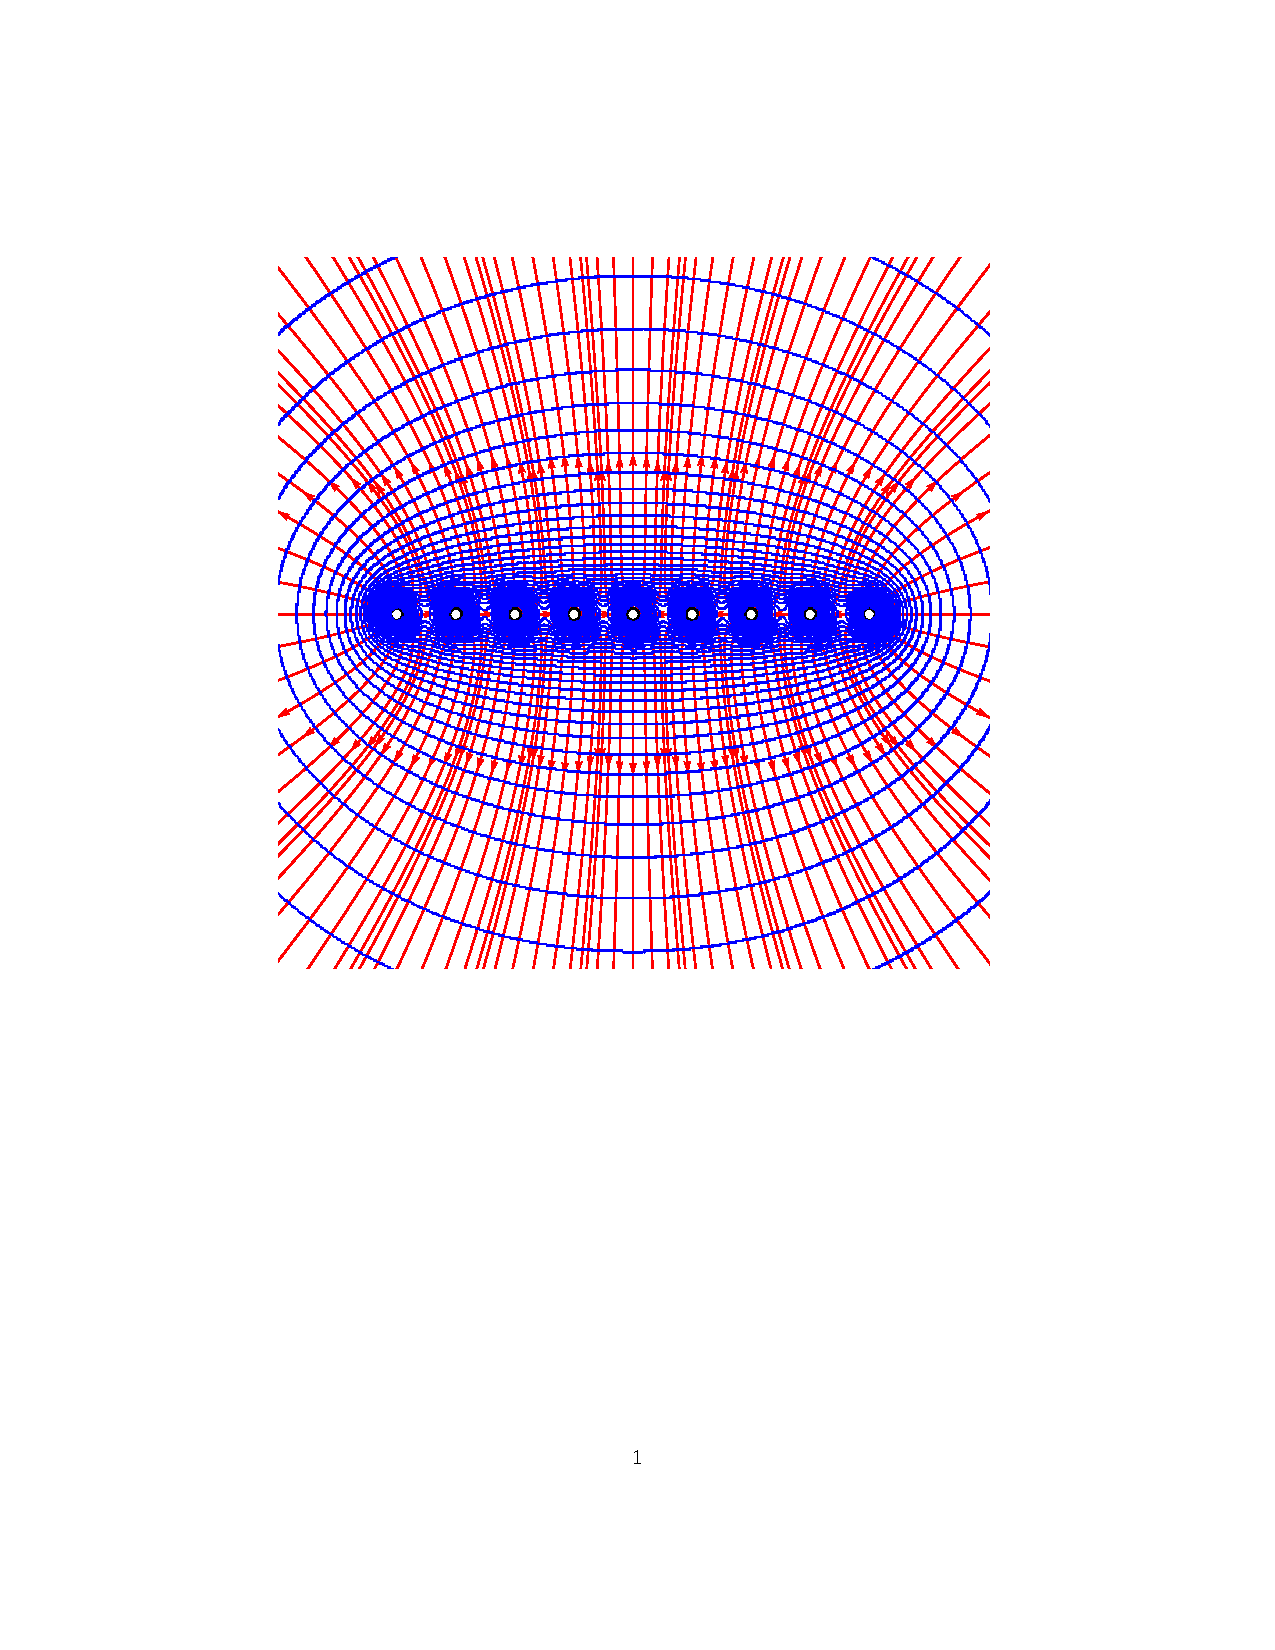
\includegraphics[width=\linewidth ,trim={6cm 14cm 6cm 7cm},clip]{Efield_graph_eq.pdf}
  \caption{Superposition of multiple positive point charges in a row}
  \label{fig:marginfig}
\end{marginfigure}
  Consider the situation of a uniform field, like that between two infinitely large charged plates.
  $$\Delta V=-\sum_A^B \overrightarrow{E}\cdot \Delta \overrightarrow{s}=-E\sum_A^B \Delta S=-E (B-A)=-ED$$
  In this case the potential varies linearly.  This is known as Ed's law.  It is generally applicable at a scale where the field is constant.
  \subsection{Point Charge}
  \begin{marginfigure}[0pt]%
  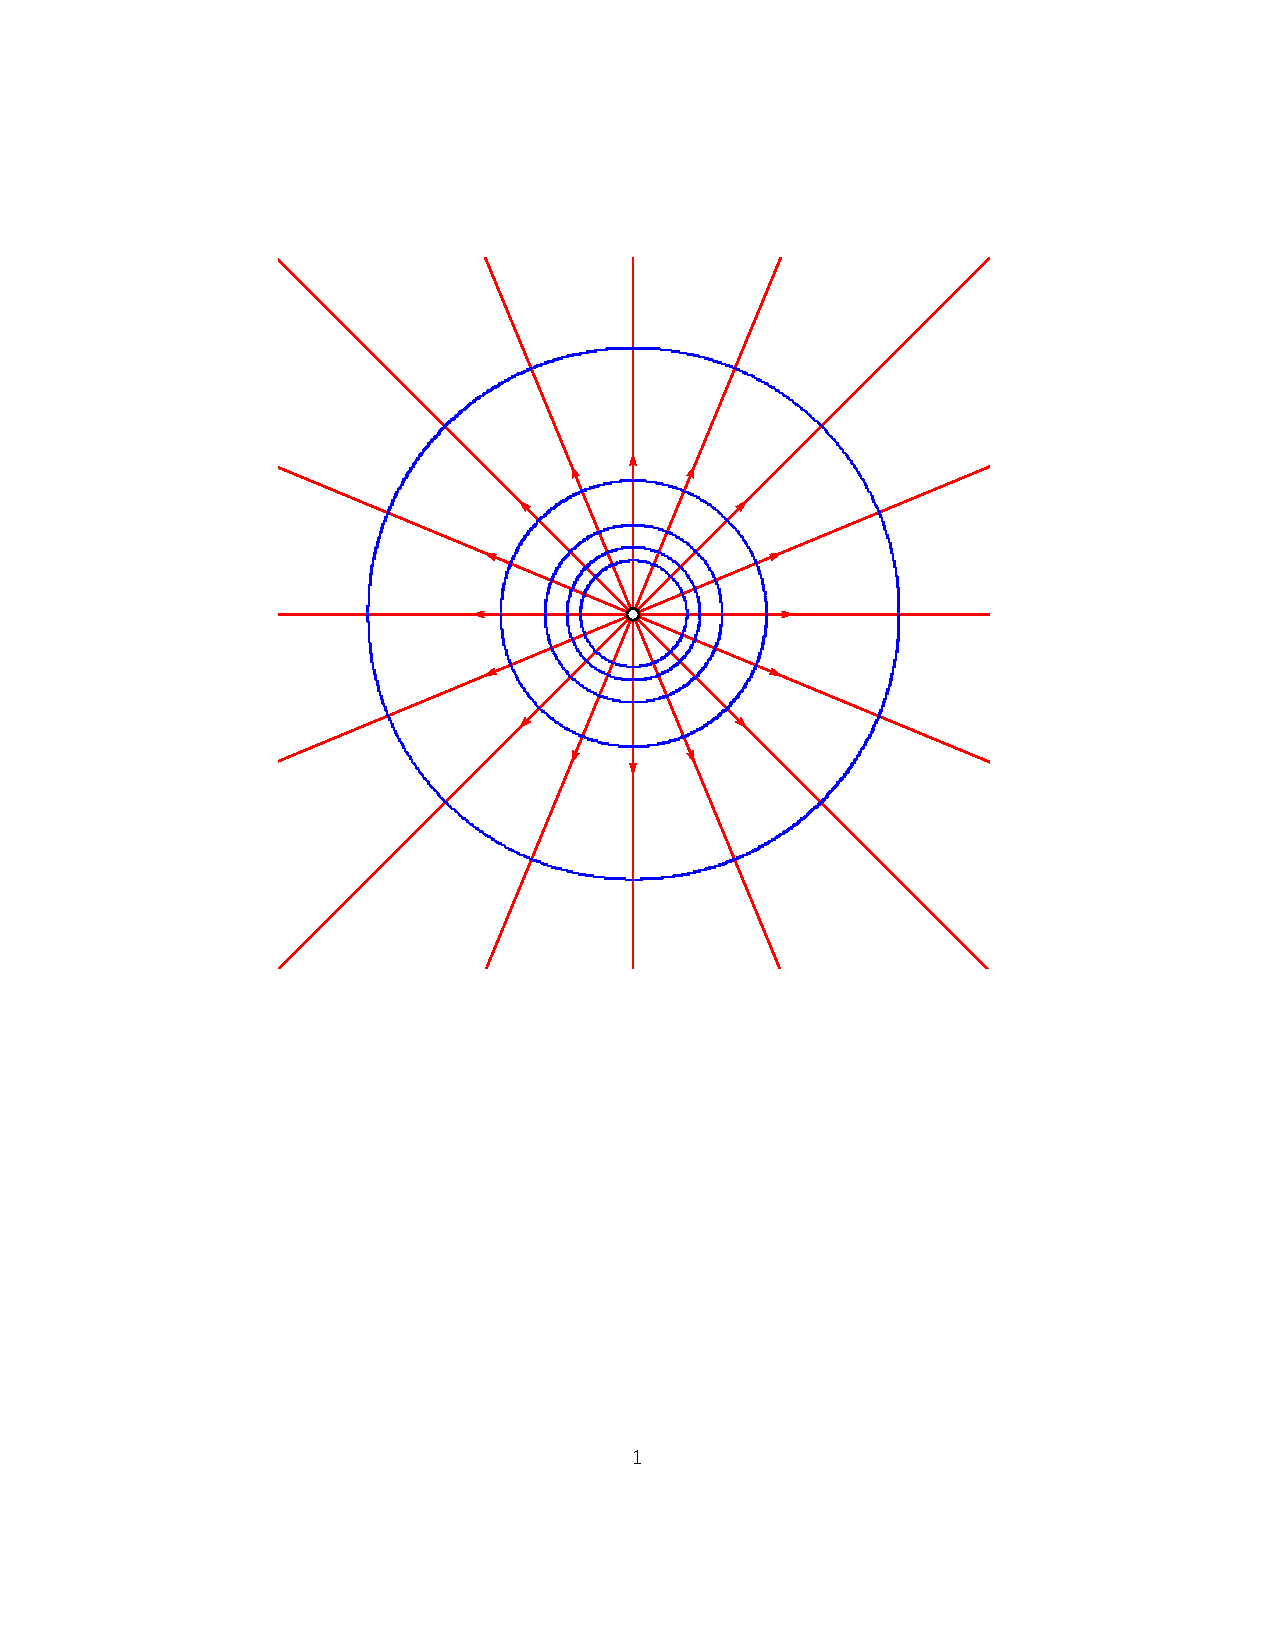
\includegraphics[width=\linewidth ,trim={7cm 14cm 7cm 7cm},clip]{Efield_graph3.pdf}
  \caption{Single positive charge with equipotential lines}
  \label{fig:marginfig}
\end{marginfigure}
  The potential around a point charge has the familiar $\frac{1}{r}$ dependence.
$$V=k_e\frac{q}{r} $$

\begin{marginfigure}[0pt]%
  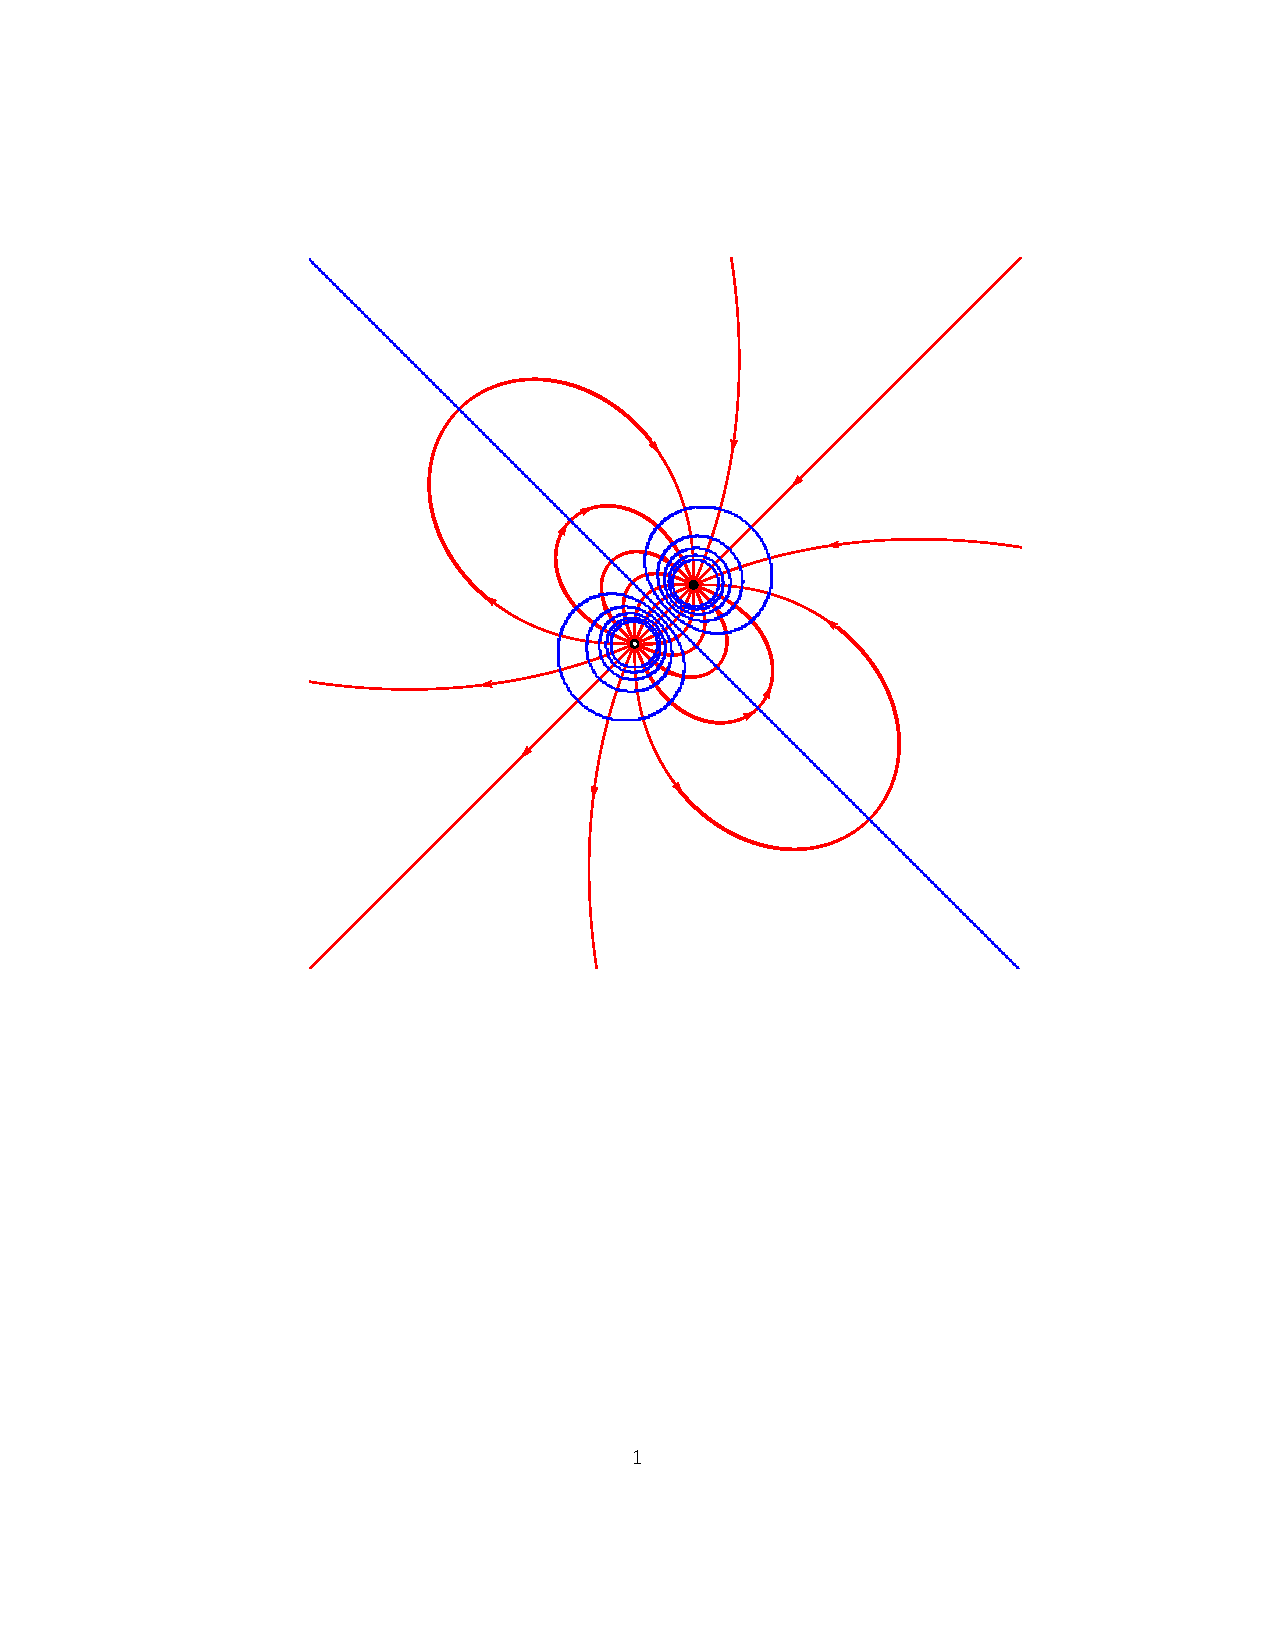
\includegraphics[width=\linewidth ,trim={7cm 14cm 7cm 7cm},clip]{dipole_graph_eq.pdf}
  \caption{Dipole field with equipotential lines}
  \label{fig:marginfig}
\end{marginfigure}

\subsection{Superposition of Point Charges}
$$V=k_e\sum_{i=1}^{N} \frac{q_i}{r_i} $$

%\subsection{Continuous Distribution}
%$$V=k_e\int \frac{dq}{r}$$



   \subsection{Vector Field, Scalar Field and Gradient}
     $$\overrightarrow{E}=-\lim_{\Delta \rightarrow 0}\left[\begin{array}{c} \nicefrac{\Delta V}{\Delta x} \\ \nicefrac{\Delta V}{\Delta y} \\ \nicefrac{\Delta V}{\Delta z}\end{array}\right]=-\lim_{\Delta \rightarrow 0}\left[\begin{array}{c} \nicefrac{\Delta }{\Delta x} \\ \nicefrac{\Delta }{\Delta y} \\ \nicefrac{\Delta }{\Delta z}\end{array}\right]V=-\nabla{V}$$
   \subsection{Equipotential Surfaces}
   Equipotential lines, or surfaces in 3-D, are equivalent to contour lines on a topographical map showing lines of equal elevation.
   \begin{itemize}
   \item An equipotential surface is any surface consisting of a continuous distribution of points held at the same electric potential.
   \item Electric field lines intersect equipotential lines at right angles.  They are perpendicular.
   \item Connected conductors share the same potential value.
   \end{itemize} 

\chapter{Circuits \& Current}

\textit{Where there is power, there is resistance.}\\
\noindent\textbf{-   Michel Foucault}

\vspace{1cm}

\begin{marginfigure}%
  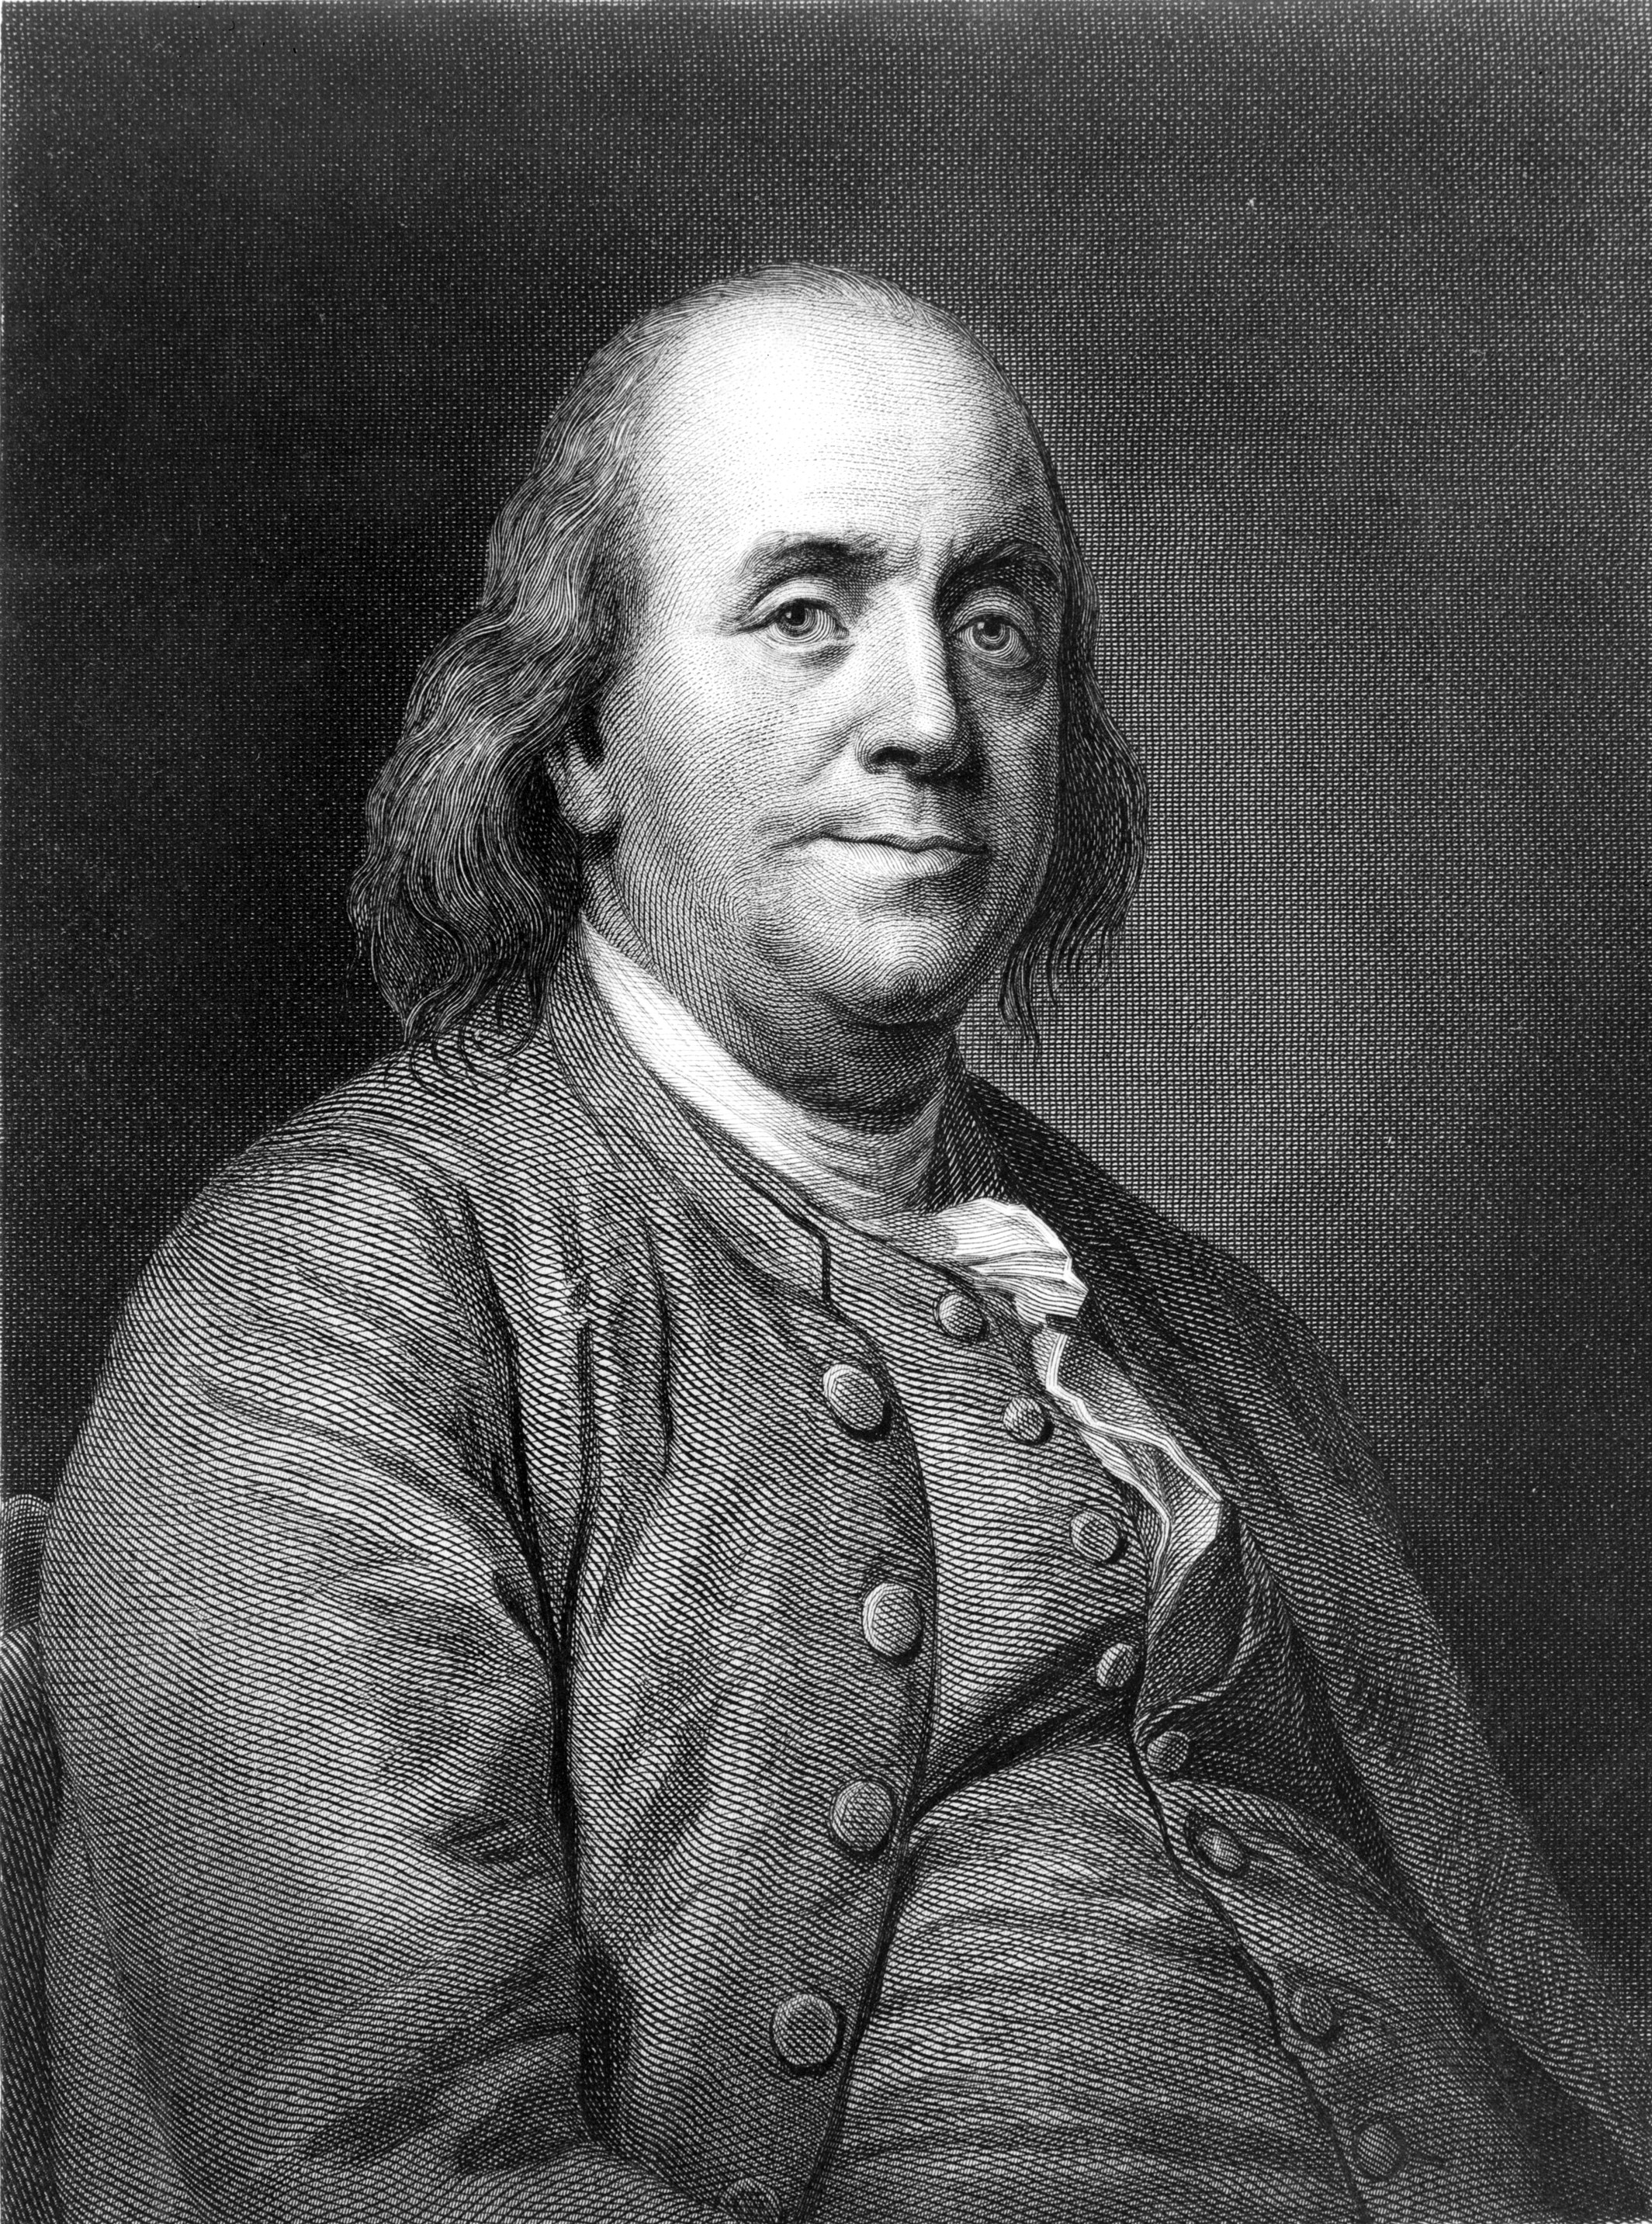
\includegraphics[width=\linewidth]{ben.jpg}
  \caption{Benjamin Franklin $\heartsuit$'s electricity}
  \label{fig:marginfig}
\end{marginfigure}

\section{Capacitance}
A capacitor holds a charge $+Q$ and $-Q$ on two plates at a given separation.   There is a voltage difference between the two plates $V$.
Capacitance is the ability of a body to store an electrical charge. A material with a large capacitance holds more electric charge at a given voltage, than one with low capacitance.  It is defined as the charge stored per volt.
$$C\equiv\frac{Q}{V}$$
The unit of capacitance is the farad.
$$1\ \text{Farad}=\frac{\text{Coulomb}}{\text{Volt}}$$
Consider the capacitor holding charges $+Q$ and $-Q$ on two plates.  Each has an area $A$ and they are separated by a distance $d$.  The constant electric field $E$ and and voltage difference $V$ are given as follows. 
$$E=\frac{\sigma}{\epsilon_0}=\frac{Q}{A\epsilon_0} \hspace{2cm} V=Ed$$
In this context the capacitance may be written in terms of the plate area and the separation distance.  
$$C=\frac{\epsilon_0A}{d}$$
In other words, the capacitance is strictly a feature of the structure of the capacitor and not a function of the particular voltage it is held at or how much charge is on it for the given conditions.

\newpage
\begin{marginfigure}%
  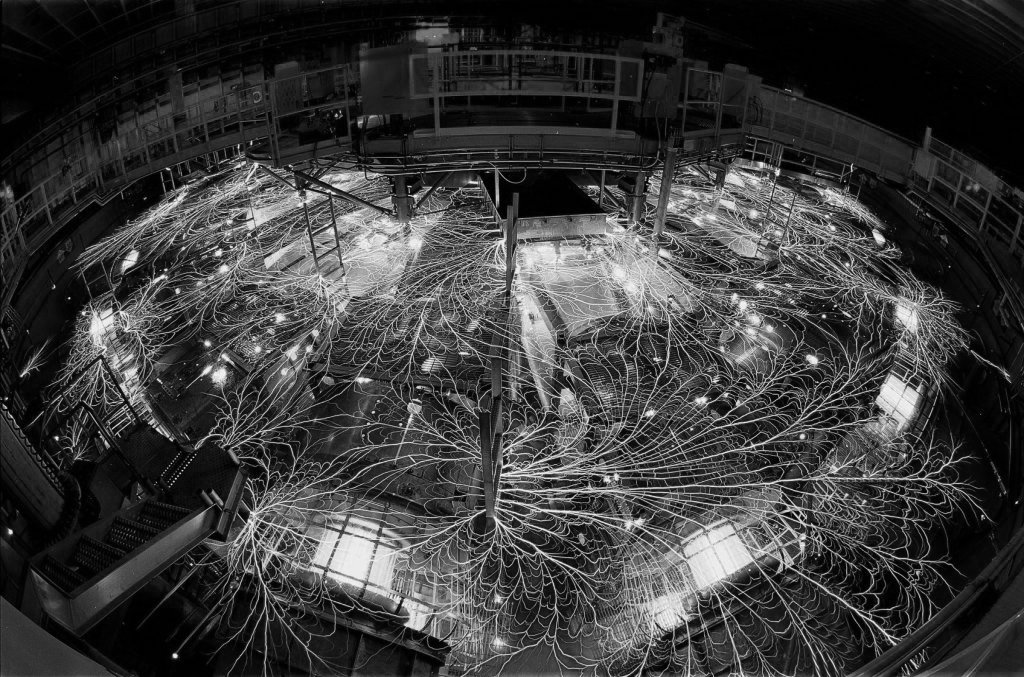
\includegraphics[width=\linewidth]{z-machine.jpg}
  \caption{The Z machine}
  \label{fig:marginfig}
\end{marginfigure}

\marginnote[30pt]{For a few billionths of a second the Z machine uses 80 times the entire world's electrical power output.}
\section{Circuit Combinations}
\subsection{Parallel}
Since the electrostatic force is conservative the voltage drop between two points should be independent of path.  Therefore the voltage drop across parallel capacitors should be equal.
$$V=V_1=V_2$$
In addition collapsing parallel capacitors into a single equivalent capacitor would have the charges add.
$$Q_{eq}=Q_1+Q_2$$
Substituting for each $Q$ using $Q=CV$ yields the next equation.
$$ C_{eq} V=C_1 V_1+C_2 V_2$$
Cancelling each of the equivalent voltages gives the following capacitance addition rule for parallel capacitors.
$$C_{eq}=C_1+C_2$$
$$\begin{circuitikz} 
\draw
(0,0) to[battery] (2,0) -- (2,2)
      to[capacitor, l=$C_1$] (0,2) -- (0,0);
      \draw (2,2) -- (2,4) to[capacitor, l=$C_2$] (0,4) -- (0,2);
\end{circuitikz}
\hspace{1cm} \text{equivalent to} \hspace{1cm} 
\begin{circuitikz} 
\draw
(0,0) to[battery] (2,0) -- (2,2)
      to[capacitor, l=$C_{eq}$] (0,2) -- (0,0);
\end{circuitikz}$$

\subsection{Series}
When capacitors are in series the voltages add to the total voltage of the circuit path.
$$V=V_1+V_2$$
The charges $Q_1$ and $Q_2$ are equal.  This is apparent when considering the floating circuit element shared by the two capacitors but completely isolated from the rest of the circuit.  Before the voltage is applied the charge in it is zero.  Once the voltage of the battery is applied the charge segregates, $+Q$ to one side and $-Q$ to the other side, conserving the total charge of zero.  Therefore the charge on the equivalent capacitor is equal to that on each of the series capacitors.
$$Q_{eq}=Q_1=Q_2$$
Starting with the voltage addition equation and substituting $V=\frac{Q}{C}$ for each component yields the following.
$$\frac{Q_{eq}}{C_{eq}}=\frac{Q_1}{C_1}+\frac{Q_2}{C_2}$$
Finally, cancelling the equal charge factors gives the equivalent capacitance for series capacitors.
$$\frac{1}{C_{eq}}=\frac{1}{C_1}+\frac{1}{C_2}$$
$$\begin{circuitikz} 
\draw
(0,0) to[battery] (4,0) -- (4,2)
      to[capacitor, l=$C_1$] (2,2) to[capacitor, l=$C_2$] (0,2) -- (0,0);
\end{circuitikz}
\hspace{1cm} \text{equivalent to} \hspace{1cm} 
\begin{circuitikz} 
\draw
(0,0) to[battery] (2,0) -- (2,2)
      to[capacitor, l=$C_{eq}$] (0,2) -- (0,0);
\end{circuitikz}$$

 
 \section{Dielectrics}
 A dielectric is a non-conductive material that increases the capacitance when placed between the two plates of a capacitor.
 $$C=\kappa C_0$$
 In such materials the $\epsilon$ replaces $\epsilon_0$.  
 $$\epsilon>\epsilon_0$$
 

\section{Energy Storage}
In order to determine the energy stored in a charged capacitor consider the small amount of work $w$ associated with adding a small amount of charge $\Delta q$ to a capacitor.
$$w=V \Delta q= \frac{q}{C}\  \Delta q$$
As more charge is added to the capacitor the voltage in the capacitor increases so the next small bit of charge requires more work to add than the previous.
$$W=\text{Area}(V(q))$$
$$PE=\frac{Q^2}{2C}=\frac{QV}{2}=\frac{CV^2}{2}$$

 \newpage
 
\section{Current}
\marginnote[0pt]{
$$1 \ \text{Ampere}=\frac{1\ \text{Coulomb}}{1\ \text{second}}$$
}
Electric current is the flow of charge.  It is the time rate of change of charge and is expressed in the unit of the ampere.
$$I \equiv \lim_{\Delta \rightarrow 0}\frac{\Delta Q}{\Delta t} \hspace{2cm} Q=\text{Area(I(t))}$$


Imagine setting up a toll both where the amount of charge flowing through the gate is counted per unit time.  This is current.
\subsection{Charge Carrier}
\marginnote[0pt]{
\begin{itemize}
\item n (carrier density)
\item q (carrier charge)
\item v (carrier velocity)
\item A (cross sectional area)
\end{itemize}
}
In electric circuits this charge is often carried by moving electrons in a wire. It can also be carried by ions in an electrolyte, or by both ions and electrons such as in a plasma.  The mobile charged body is known as the charge carrier.  The current can be determined by the number of charge carriers $N$ multiplied by the carrier charge $q$ per unit time $\Delta t$.
$$I=\frac{\Delta Q}{\Delta t}=\frac{N q}{\Delta t}$$
This can be expressed in terms of the the carrier density $n$.  This is the number of charge carriers per unit volume.
$$I=\frac{\Delta Q}{\Delta t}=\frac{n q}{\Delta t}V=nq\frac{\Delta x}{\Delta t}A=nqvA$$


\subsection{Current Density}
Current density $J$ is defined as the current passing through a cross-sectional area $A$.
$$J \equiv \frac{I}{A}=nqv$$

\section{Resistance \& Ohm's Law}
\marginnote[0pt]{
\begin{itemize}
\item $\sigma$ (conductivity)
\item $\rho$ (resistivity)
\item $l$ (length)
\item $R$ (resistance)
\end{itemize}
}
In an Ohmic material the current density is proportional to the electric field in the conductor.  The constant of proportionality $\sigma$ is known as the passivity.  
$$J=\sigma E$$
Starting fwith the above equation substitute the definition of current density and $E=\frac{V}{l}$ where $l$ is the length of the circuit element.
$$J=\frac{I}{A}=\sigma E=\sigma \frac{V}{l}$$
\marginnote[0pt]{
$$1\ \Omega=1 \ \text{Ohm}=\frac{1\ \text{Volt}}{1\ \text{Ampere}}$$
}
In circuits consisting of Ohmic materials the ratio between the voltage and the current is defined as the resistance $R$.
$$R\equiv \frac{V}{I}$$
$R$ may be expressed in terms of $\sigma$, $l$ and $A$ or the resistivity $\rho=\frac{1}{\sigma}$, the reciprocal of the passivity.
$$R=\frac{l}{\sigma A}=\rho\frac{l}{A}$$
\marginnote[-60pt]{Ohm's law is typically written as follows
$$V=IR$$}

\begin{margintable}[0pt]\index{typefaces!sizes}
  \footnotesize%
  \begin{center}
    \begin{tabular}{lc}
      \toprule
     Material & Resistivity ($\Omega\cdot \text{m}$) \\
      \midrule
     Copper     & 1.7$\times10^{-8}$  \\
    Aluminum      & 2.7$\times10^{-8}$  \\
    Tungsten (20 C)     & 5.6$\times10^{-8}$  \\
    Tungsten (1500 C)    & 5.0$\times10^{-7}$  \\
    Iron    & 9.7$\times10^{-8}$ \\
    Seawater      & 2.2$\times10^{-1}$  \\
    Blood     & 1.6  \\
    Muscle   & 1.3$\times10^{1}$  \\
    Fat      & 2.5$\times10^{1}$  \\
    Pure Water     & 2.4$\times10^{5}$  \\
    Cell Membrane     & 3.6$\times10^{7}$  \\
      \bottomrule
    \end{tabular}
  \end{center}
  \caption{A list of resistivities}
  \label{tab:font-sizes}
\end{margintable}


\section{Power}
$$P=IV$$
$$P=I^2R=\frac{V^2}{R}$$

\section{Resistors in Circuits}
\subsection{Series}
$$V=IR_1+IR_2=I(R_1+R_2)$$
$$V=IR_{eq} \hspace{2cm} R_{eq}=R_1+R_2$$

The current is the same in each resistor because any charge that flows through $R_1$ must also flow through $R_2$.

$$\begin{circuitikz} 
\draw
(0,0) to[battery] (4,0) -- (4,2)
      to[resistor, l=$R_2$] (2,2) to[resistor, l=$R_1$] (0,2) -- (0,0);
\end{circuitikz}
\hspace{1cm} \text{equivalent to} \hspace{1cm} 
\begin{circuitikz} 
\draw
(0,0) to[battery] (2,0) -- (2,2)
      to[resistor, l=$R_{eq}$] (0,2) -- (0,0);
\end{circuitikz}$$

\subsubsection{General}
$$R_{eq}=R_1+R_2+R_3 +\cdots$$

\subsection{Parallel}
The potential drop across parallel resistors is equal due to path independence of the potential function.  Additionally the total current going through each branch is conserved.
$$V=I_1R_1=I_2R_2$$
$$I=I_1+I_2$$
$$I=\frac{V}{R_1}+\frac{V}{R_2}=V\left(\frac{1}{R_1}+\frac{V}{R_1}\right)$$
$$I=\frac{V}{R_{eq}}$$
$$\frac{1}{R_{eq}}=\frac{1}{R_{1}}+\frac{1}{R_{2}}$$

$$\begin{circuitikz} 
\draw
(0,0) to[battery] (2,0) -- (2,2)
      to[resistor, l=$R_1$] (0,2) -- (0,0);
      \draw (2,2) -- (2,4) to[resistor, l=$R_2$] (0,4) -- (0,2);
\end{circuitikz}
\hspace{1cm} \text{equivalent to} \hspace{1cm} 
\begin{circuitikz} 
\draw
(0,0) to[battery] (2,0) -- (2,2)
      to[resistor, l=$R_{eq}$] (0,2) -- (0,0);
\end{circuitikz}$$
\subsubsection{General}
$$\frac{1}{R_{eq}}=\frac{1}{R_{1}}+\frac{1}{R_{2}}+\frac{1}{R_{3}}+\cdots$$

\section{Kirchoff's Rules}
\begin{itemize}
\item The sum of the currents entering a junction must be equal to the sum of the currents leaving that junction.
\item The algebraic sum of the changes in potential across all elements around any closed circuit must be zero.
\end{itemize}

\section{RC Circuits}
\marginnote[0pt]{Consider an uncharged capacitor in series with a resistor and a battery.  Initially there is no charge on it so there is no voltage drop across it.  Once the circuit is closed and the current begins to flow it begins to accumulate charge.  As it charges the rate of charging slows exponentially and approaches a maximum value asymptotically.}
$$\begin{circuitikz} 
\draw
(0,0) to[battery] (4,0) to[closing switch] (4,2)
      to[resistor, l=$R$] (2,2) to[capacitor, l=$C$] (0,2) -- (0,0);
\end{circuitikz}
$$

%$$V=V_R+V_C$$
%$$V=IR+\frac{q}{C}$$
%$$\frac{V}{R}=\frac{dq}{dt}+\frac{q}{RC}$$
%$$\int \frac{-dt}{RC}=\int \frac{dq}{q-CV}$$
\marginnote[50pt]{Consider an charged capacitor in series with a resistor and no battery.  Initially there is maximal charge on it so there maximal voltage drop across it.  Once the circuit is closed charge begins to flow of the capacitor.  As it discharges the rate slows exponentially and approaches a zero asymptotically.}
\subsection{Charging a Capacitor}
$$q(t)=CV(1-e^{-\frac{t}{RC}})=Q(1-e^{-\frac{t}{RC}})$$
$$I(t)=\frac{V}{R}e^{-\frac{t}{RC}}$$
\subsection{Discharging a Capacitor}
$$q(t)=Qe^{-\frac{t}{RC}}$$
$$I(t)=I_0e^{-\frac{t}{RC}}$$


\chapter{Magnetism}

\textit{What magnetism is, no-one knows. We can only think of it as a peculiar condition created in space by the motion of electricity.}\\
\noindent\textbf{-   Sydney Evershed}

\vspace{1cm}


\begin{marginfigure}%
  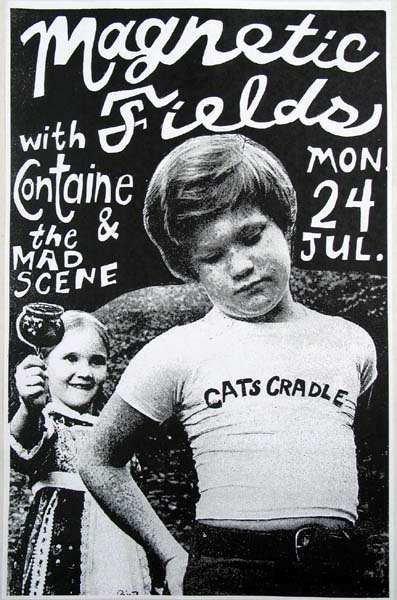
\includegraphics[width=\linewidth]{mag_fields.jpg}
  \caption{Magnetic Fields concert poster}
  \label{fig:marginfig}
\end{marginfigure}

Magnetism is the phenomenon of current interactions.  A current moving through space applies a force to other currents around it.  The story of magnetism is one of the deeper mysteries in physics.  As in electrostatics, physics uses the construct of the vector field to narrate the force interaction.

Currents generate magnetic fields in the space around them.  Currents also interact with fields in space.  This results in a magnetic force.  The story is therefore split into two parts.  How do currents generate fields in space?  How do currents interact with fields in space?  The present narrative addresses the second question first.


\section{Magnetic Force/Field}
Consider a a magnetic field in space $\overrightarrow{B}(\overrightarrow{r})$ and a particle with charge $q$ and velocity $\overrightarrow{v}$.   The resulting magnetic force is represented using the vector cross product.

$$\overrightarrow{F}_{B}=q\overrightarrow{v}\times \overrightarrow{B}$$
Remember the magnitude of the cross product is proportional to the $\sin$ of the angle between the field vector and the velocity vector.
$$F_{B}=qvB \sin \theta$$

\begin{marginfigure}[10pt]
 
\tdplotsetmaincoords{60}{110}
\begin{tikzpicture}[scale=1,tdplot_main_coords]
\coordinate (O) at (0,0,0);
\coordinate (P) at (1,2,3);

\draw[very thick,->] (0,0,0) -- (-2,2,0) node[anchor=south ]{$B$};
\draw[very thick,->] (0,0,0) -- (0,4,0) node[anchor=north west]{$v$};
\draw[very thick,->] (0,0,0) -- (0,0,3) node[anchor=south]{$F_{B}$};
\fill (0,0,0) circle(1mm) node[anchor=north east]{$q$};
%draw a vector from origin to point (P) 
\draw (-0.6,1.2,0) node[anchor=center,color=black]{$\theta$};


%draw projection on xy plane, and a connecting line
%syntax: \tdplotdrawarc[coordinate frame, draw options]{center point}{r}{angle}{label options}{label}
%\tdplotdrawarc{(O)}{0.2}{0}{\phivec}{anchor=north}{$\phi$}


%set the rotated coordinate system so the x'-y' plane lies within the
%"theta plane" of the main coordinate system
%syntax: \tdplotsetthetaplanecoords{\phi}
%\tdplotsetthetaplanecoords{\phivec}

%draw theta arc and label, using rotated coordinate system
%\tdplotdrawarc[tdplot_rotated_coords]{(0,0,0)}{0.5}{0}{\thetavec}{anchor=south west}{$\theta$}

\end{tikzpicture}

  \caption{Force of a moving charged particle in a magnetic field}
  \label{fig:marginfig}
\end{marginfigure}


\subsection{Unit}
The SI unit of magnetic field is the Tesla, named after Serbian-American mad scientist Nikola Tesla.
$$1 \ \text{Tesla}=\frac{1\ \text{Newton}}{1\ \text{Ampere} \cdot \text{meter}}$$

\newpage
\begin{marginfigure}%
  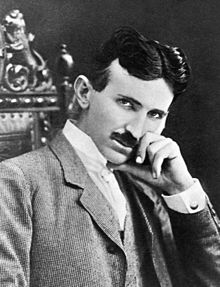
\includegraphics[width=\linewidth]{tesla.jpg}
  \caption{Handsome: Nikola Tesla}
  \label{fig:marginfig}
\end{marginfigure}


\subsection{No Work}
Since the magnetic force is always perpendicular to the velocity (displacement) no work is done by a static magnetic field on a moving particle.
$$W_B=\sum \overrightarrow{F}_B\cdot \ \Delta\overrightarrow{s}=\sum \overrightarrow{F}_B\cdot\overrightarrow{v}\ \Delta t=0$$
Fields may do work on magnetic dipoles, namely loops of current, but these are rigid bodies.  A constant magnetic field does not work on a single moving charged particle.
\section{Magnetic Force on a Straight Wire }
For $N$ charges particle in wire of length $L$ and cross-sectional area $A$, the total force on the wire is given as follows.

$$\overrightarrow{F}_{wire}=Nq\overrightarrow{v}\times \overrightarrow{B}= (nAL)q\overrightarrow{v}\times \overrightarrow{B}$$ 
Recall the expression for current as a charge rate of flux.  
$$I=nqvA=\overrightarrow J \cdot \overrightarrow A $$
In this way the force can be expressed in terms of the current and the length of the wire.  Since the force is a vector product each factor in the product must be a vector.  since the current is technically a scalar we vectorize the length in the notation.  Of course a length by itself is not a true vector but rather a pseudo-vector.  The sign which lifts the ambiguity for the direction of the $\overrightarrow{L}$ vector is borrowed from the sign of the scalar current $I$.
$$\overrightarrow{F}_{wire}=I\overrightarrow{L}\times\overrightarrow{B} $$


\begin{marginfigure}%
  
 \tikzset{->-/.style={decoration={
  markings,
  mark=at position #1 with {\arrow{latex}}},postaction={decorate}}}
  
\begin{tikzpicture}[scale=1]
\draw[very thick,->-=.5] (0,3) -- (0,0) node[midway, anchor=west]{$I$};

\draw[->] (-1,0.3)--(-0.2,0.3);
\draw[->] (-1,0.5)--(-0.2,0.5);
\draw[->] (-1,0.7)--(-0.2,0.7);
\draw[->] (-1,0.9)--(-0.2,0.9);
\draw (-1,0.6) node[anchor=east]{$B$};

\begin{scope}[scale={1}, shift={(0.4,0.6)}]
\draw (0,0) circle(1.8mm);
\fill (0,0) circle(0.3mm);
\draw (0.2,0) node[anchor=west]{$F$};
\end{scope}
\end{tikzpicture}


  \caption{Magnetic force on a current carrying wire }
  \label{fig:marginfig}
\end{marginfigure}



\section{General Wire}
For a general wire of any shape the approach is to break it up into small pieces of current carrying wire $\Delta\overrightarrow{s}$ and calculate the force $\Delta\overrightarrow{F}_{wire}$ on each piece.  We use the variable $i$ as an index for the pieces. 
$$\Delta\overrightarrow{F}_{i}=I\ \Delta\overrightarrow{s}_i\times\overrightarrow{B}(\overrightarrow{r}_i) $$
To calculate the total force a sum over the index $i$ is taken.  This add up all the little vector forces into a total force vector $\overrightarrow{F}_{wire}$.
$$\overrightarrow{F}_{wire}=\sum_i \Delta\overrightarrow{F}_{i}=\sum_i I\ \Delta\overrightarrow{s}_i\times\overrightarrow{B} (\overrightarrow{r}_i)$$
\newpage

\marginnote{One of the first drawings of a magnetic field, by Ren� Descartes, 1644. It illustrated his theory that magnetism was caused by the circulation of tiny helical particles, "threaded parts", through threaded pores in magnets.}

\begin{marginfigure}[20pt]%
  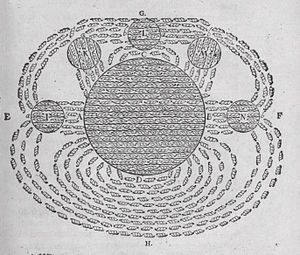
\includegraphics[width=\linewidth]{descartes_field.jpg}
  \caption{Descartes 1644 representation of the magnetic field}
  \label{fig:marginfig}
\end{marginfigure}

\subsection{Uniform Static Field: Path Independence}
A uniform and static magnetic field is constant over space and time.  $\overrightarrow{B} (\overrightarrow{r}_i)=\overrightarrow{B} $ so the summation is only on the path elements and dependent on spatial variation in the magnetic field. Such a field generates no net force.
$$\overrightarrow{F}_{wire}=I \left(\sum_a^b \ \Delta\overrightarrow{s} \right) \times\overrightarrow{B} =I\overrightarrow{s}_{ab}\times\overrightarrow{B} $$
 Such a field generates no net force.  This is because a loop has the same beginning point and end point.
$$\overrightarrow{F}_{wire}=I \left(\sum_a^a \ \Delta\overrightarrow{s} \right) \times\overrightarrow{B}=0 $$


\section{Torque on a Current Loop}
 
 \begin{marginfigure}[20pt]%

 
 \tikzset{->-/.style={decoration={
  markings,
  mark=at position #1 with {\arrow{latex}}},postaction={decorate}}}
  
\begin{tikzpicture}[scale=1]
\draw[very thick,->-=.5] (0,0) -- (2,0);
\draw[very thick,->-=.5] (2,0) -- (2,3)node[midway, anchor=west]{$I$};
\draw[very thick,->-=.5] (2,3) -- (0,3) ;
\draw[very thick,->-=.5] (0,3) -- (0,0);
\draw[->] (-1,0.3)--(-0.2,0.3);
\draw[->] (-1,0.5)--(-0.2,0.5);
\draw[->] (-1,0.7)--(-0.2,0.7);
\draw[->] (-1,0.9)--(-0.2,0.9);
\draw (-1,0.6) node[anchor=east]{$B$};

\begin{scope}[scale={1}, shift={(-0.4,2.4)}]
\draw (0,0) circle(1.8mm);
\fill (0,0) circle(0.3mm);
\draw (-0.2,0) node[anchor=east]{$F_1$};
\end{scope}

\begin{scope}[scale={1}, shift={(2.4,2.4)}]
\draw (0,0) circle(1.8mm);
\fill (0,0) circle(0.3mm);
\draw (0.2,0) node[anchor=west]{$F_2$};
\begin{scope}[scale={1}, rotate={(45)}]
\draw(-0.18,0) -- (0.18,0);
\draw(0,-0.18) -- (0,0.18);
\end{scope}
\end{scope}
\end{tikzpicture}

  \caption{Torque on a closed loop}
  \label{fig:marginfig}
\end{marginfigure}
While the total force is zero for a uniform magnetic field on a closed current loop there is a net torque on the loop.  Consider a rectangular loop of current with area $A$ and uniform magnetic field $B$.  The total torque is the product of the area and the magnetic field. 
$$ \tau=IAB$$
$$ \overrightarrow{\tau}=I\overrightarrow{A}\times \overrightarrow{B}$$
\subsection{Magnetic Moment}
The magnetic moment is defined as product of the current and the area.  Note that the current is a scalar and area is a vector.  Thus the magnetic moment is a vector quantity.
$$\overrightarrow{\mu}= I \overrightarrow{A}$$
The torque on the loop may be parameterized in terms of the magnetic moment.
$$\overrightarrow{\tau}=\overrightarrow{\mu}\times \overrightarrow{B}$$
\section{Homopolar Electric Motor}
The homopolar motor was the first electrical motor to be built. Its operation was demonstrated by Michael Faraday in 1821 at the Royal Institution in London.  It is driven by a Lorentz force.  A paper clip, AAA battery and permanent magnet constitute a homopolar motor.
\begin{marginfigure}[-180pt]%
  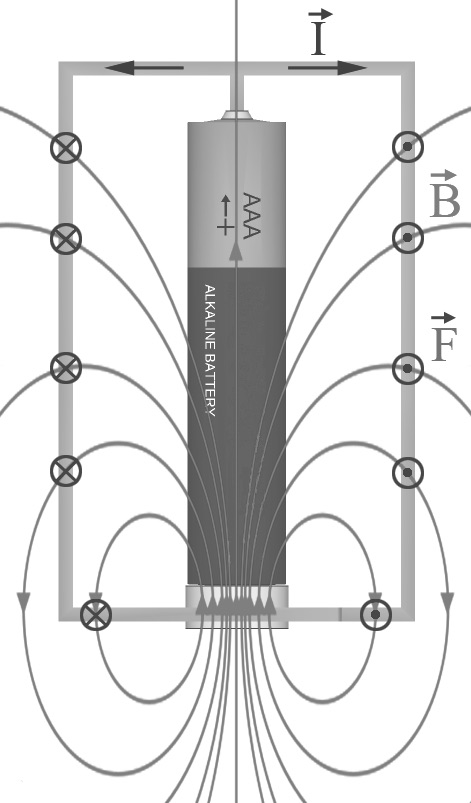
\includegraphics[width=\linewidth]{homopolar_motor.jpg}
  \caption{Simple homopolar motor}
  \label{fig:marginfig}
\end{marginfigure}


\newpage
\section{Circular Motion of a Charged Particle in a Uniform B Field}
\begin{marginfigure}[0pt]%
  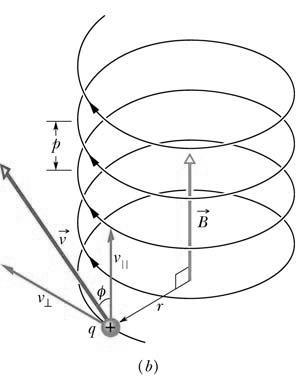
\includegraphics[width=\linewidth]{helix.jpg}
  \caption{Helical motion of a charged particle in a magnetic field}
  \label{fig:marginfig}
\end{marginfigure}
$$F_B=F_c$$
$$ qv_{\perp}B=\frac{mv_{\perp}^2}{r}$$
$$\frac{v_{\perp}}{r}=\omega=\frac{qB}{m}$$
\section{General Motion}
The total force on an electric field and magnetic field on a moving charged particle is known as the Lorentz force.
$$\overrightarrow{F}=q\overrightarrow{E}+q\overrightarrow{v}\times\overrightarrow{B}$$
\section{Velocity Selector}
For perpendicular electric and magnetic fields the Lorentz force will be zero on particle on a particle traveling with a perpendicular component of velocity equal to the ratio of electric field to magnetic field.
$$\overrightarrow{E}=E\hat{x} \hspace{1cm} \overrightarrow{B}=B\hat{y} \hspace{1cm} \overrightarrow{v}=v\hat{z}$$
$$\overrightarrow{F}=qE\hat{x}+qvB\hat{z}\times\hat{y}=q(E-vB)\hat{x}$$
$$v=\frac{E}{B}$$

\begin{marginfigure}
  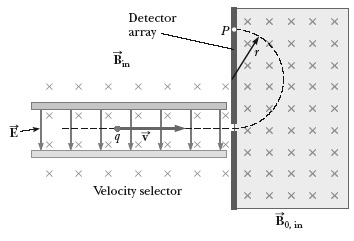
\includegraphics[width=\linewidth]{selector.jpg}
  \caption{Mass spectroscopy with a velocity selector and a detector plate in a constant magnetic field }
  \label{fig:marginfig}
\end{marginfigure}


\section{Mass Spectroscopy}
Mass spectroscopy leverages the physics of the velocity selector and circular motion in a magnetic field to precisely measure mass to charge ratio.  The radius of curvature of the particle is $r$.
$$r=\frac{mv}{qB}$$
Therefore measuring the electric field, magnetic field and radius of curvature would determine the mass to charge ratio of the particle.

$$\frac{m}{q}=\frac{rB}{v}=\frac{rB^2}{E}$$ 
\section{Sources of Magnetic Field}
Up until now there have only been description of currents interacting with existing magnetic fields.  The second half of the story of magnetism addresses how those fields are generated.

The general law for determining the magnetic field in space $\overrightarrow{B}(\overrightarrow{r})$ generated by a current through a general wire is complex and cumbersome.  We begin with a description of the little bit of magnetic field $ \Delta \overrightarrow{B}$ generated by a current $I$ traveling through a small length of wire $\overrightarrow{s}$.  The vector from the the section of wire to the point in space is $\overrightarrow{r}$.  This is known as the Biot-Savart law.
$$\text{Biot-Savart Law} \hspace{2cm} \Delta \overrightarrow{B}=k_m\frac{I\ \Delta\overrightarrow{s}\times \hat{r}}{r^2}$$
There is a constant of proportionality $k_m$ analogous to the $k_e$ for electric fields.  We may also parameterize this constant in terms of the magnetic permeability of free space $\mu_0$.
$$k_m=\frac{\mu_0}{4\pi} =10^{-7}\  \frac{\text{Tm}}{\text{A}}$$
$$\text{Magnetic Permeability of Free Space} \hspace{2cm} \mu_0=4\pi\times10^{-7}\  \frac{\text{Tm}}{\text{A}}$$
In order to get the magnetic field at a point in space all the  contributions from all the small bits of wire must be summed up.
$$\overrightarrow{B}=\sum \Delta \overrightarrow{B}= \frac{\mu_0I}{4\pi}\sum \frac{\Delta\overrightarrow{s}\times \hat{r}}{r^2}$$

\section{B Field Around an Infinitely Long Straight Wire}
Consider a long straight wire carrying a current $I$.  We cut cut the wire into little pieces of length $\Delta x$ each having an angle$\theta$ with the point in question a distance $a$ away from the wire.  The contribution of each segment of wire is given here.
$$\Delta B=\frac{\mu_0I}{4\pi}\frac{\Delta x\ \sin\theta}{r^2}$$
The contributions from all the pieces of wire gives a total magnetic field at the point in question proportional to one over the distance.
$$B=\frac{\mu_0I}{2\pi a}$$
\section{B Field Above a Current Loop}
The magnetic field a distance $x$ above a loop of current, with radius $R$, is derived as follows.
$$\Delta B=\frac{\mu_0I}{4\pi}\frac{|\Delta\overrightarrow{s}\times \hat{r}|}{r^2}=\frac{\mu_0I}{4\pi}\frac{\Delta s}{x^2+R^2}$$
The sum of all the components yields the following.
$$B=\frac{\mu_0IR^2}{2(x^2+R^2)^{3/2}}$$
In the limit of the distance much larger than the radius, $x>>R$, we get the following.
$$B=\frac{\mu_0IR^2}{2x^3}$$
\begin{marginfigure}
  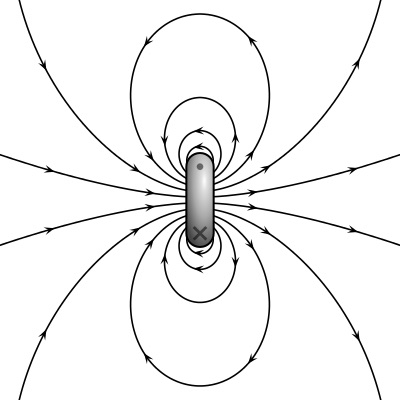
\includegraphics[width=\linewidth]{mag_dipole.jpg}
  \caption{Magnetic field around a loop of current}
  \label{fig:marginfig}
\end{marginfigure}
\section{Magnetic Force Between Two Parallel Wires}
Consider the force between two parallel wires.
$$\frac{F_1}{l}=\frac{\mu_0I_1I_2}{2\pi a}$$
This force is attractive if the the currents are in the same direction and repulsive if the wires are in opposite directions.

\section{Ampere's Law}
Ampere's law is the elegant representation describing the magnetic field around a current $I$.  We use an Amperian loop $s$ as a tool to determine the magnetic field 
$$\sum_{closed} \overrightarrow{B}\cdot \Delta\overrightarrow{s}=\mu_0I$$ 
The line integral of $\overrightarrow{B}\cdot \Delta\overrightarrow{s}$ around any closed path equals $\mu_0I$, where I is the total steady state current 
passing through any surface bounded by the closed path Amperian loop.
\subsection{Symmetric Path and Field}
If the field is uniform along the closed path then the summation reduces.
$$BS=\mu_0I$$ 
\section{B Field Inside a Solenoid}
A solenoid is a winding loop of current.  The magnetic field inside a solenoid maybe easily determined using Ampere's law using a rectangular loop of length $l$.
$$\sum_{closed} \overrightarrow{B}\cdot \Delta \overrightarrow{s}=Bl$$
$N$ is the number of winding turns through the loop.
$$Bl=\mu_0NI$$
It reduces to a linear dependence on the the density of turns per unit length $n$.
$$B=\mu_0nI$$

\section{Magnetic Flux}
Magnetic flux is defined as the total amount of magnetic field going through a surface.
$$\Phi_B=\sum \overrightarrow{B}\cdot d \overrightarrow{A}$$
The total magnetic flux going through a closed surface is zero.  This is known as Gauss's law for magnetism.
$$\sum_{closed} \overrightarrow{B}\cdot \Delta\overrightarrow{A}=0$$

\section{Displacement Current}
Displacement current is the effective current generated at a capacitor gap.  It is proportional to the time rate of change of electric flux.
$$I_d\equiv\epsilon_0\frac{d\Phi_E}{dt}$$
Since Ampere's law involves determining the current flux though the membrane bound by the Amperian loop is is possible to stretch the membrane so that it passed through the capacitor gap, where no actual current would pass through the membrane.  Therefore an increasing electric field must be considered equivalent to a real current.
$$\sum_{closed} \overrightarrow{B}\cdot \Delta \overrightarrow{s}=\mu_0(I+I_d)$$
An increasing electric field generates a magnetic field around it.  Therefore Ampere law requires a small addendum to include the displacement current.


\chapter{Induction}

\textit{I was at first almost frightened when I saw such mathematical force made to bear upon the subject, and then wondered to see that the subject stood it so well.}\\
\noindent\textbf{-   Michael Faraday}

\vspace{1cm}


\begin{marginfigure}%
  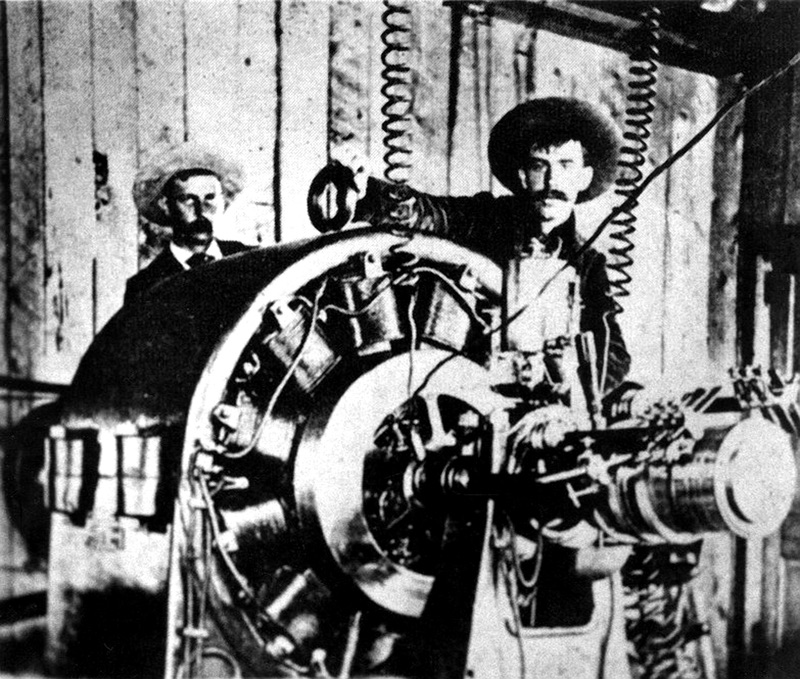
\includegraphics[width=\linewidth]{generator.jpg}
  \caption{Dudes posing with their Westinghouse alternator in 1891}
  \label{fig:marginfig}
\end{marginfigure}


\marginnote[20pt]{
\section{Magnetic Flux}
Magnetic flux $\Phi_B$ is the is the sum of magnetic field $\overrightarrow{B}$ passing through a surface area $\overrightarrow{A}$.
$$ \Phi_B=\sum\overrightarrow{B}\cdot \Delta\overrightarrow{A}$$ }


\begin{marginfigure}[20pt]%
  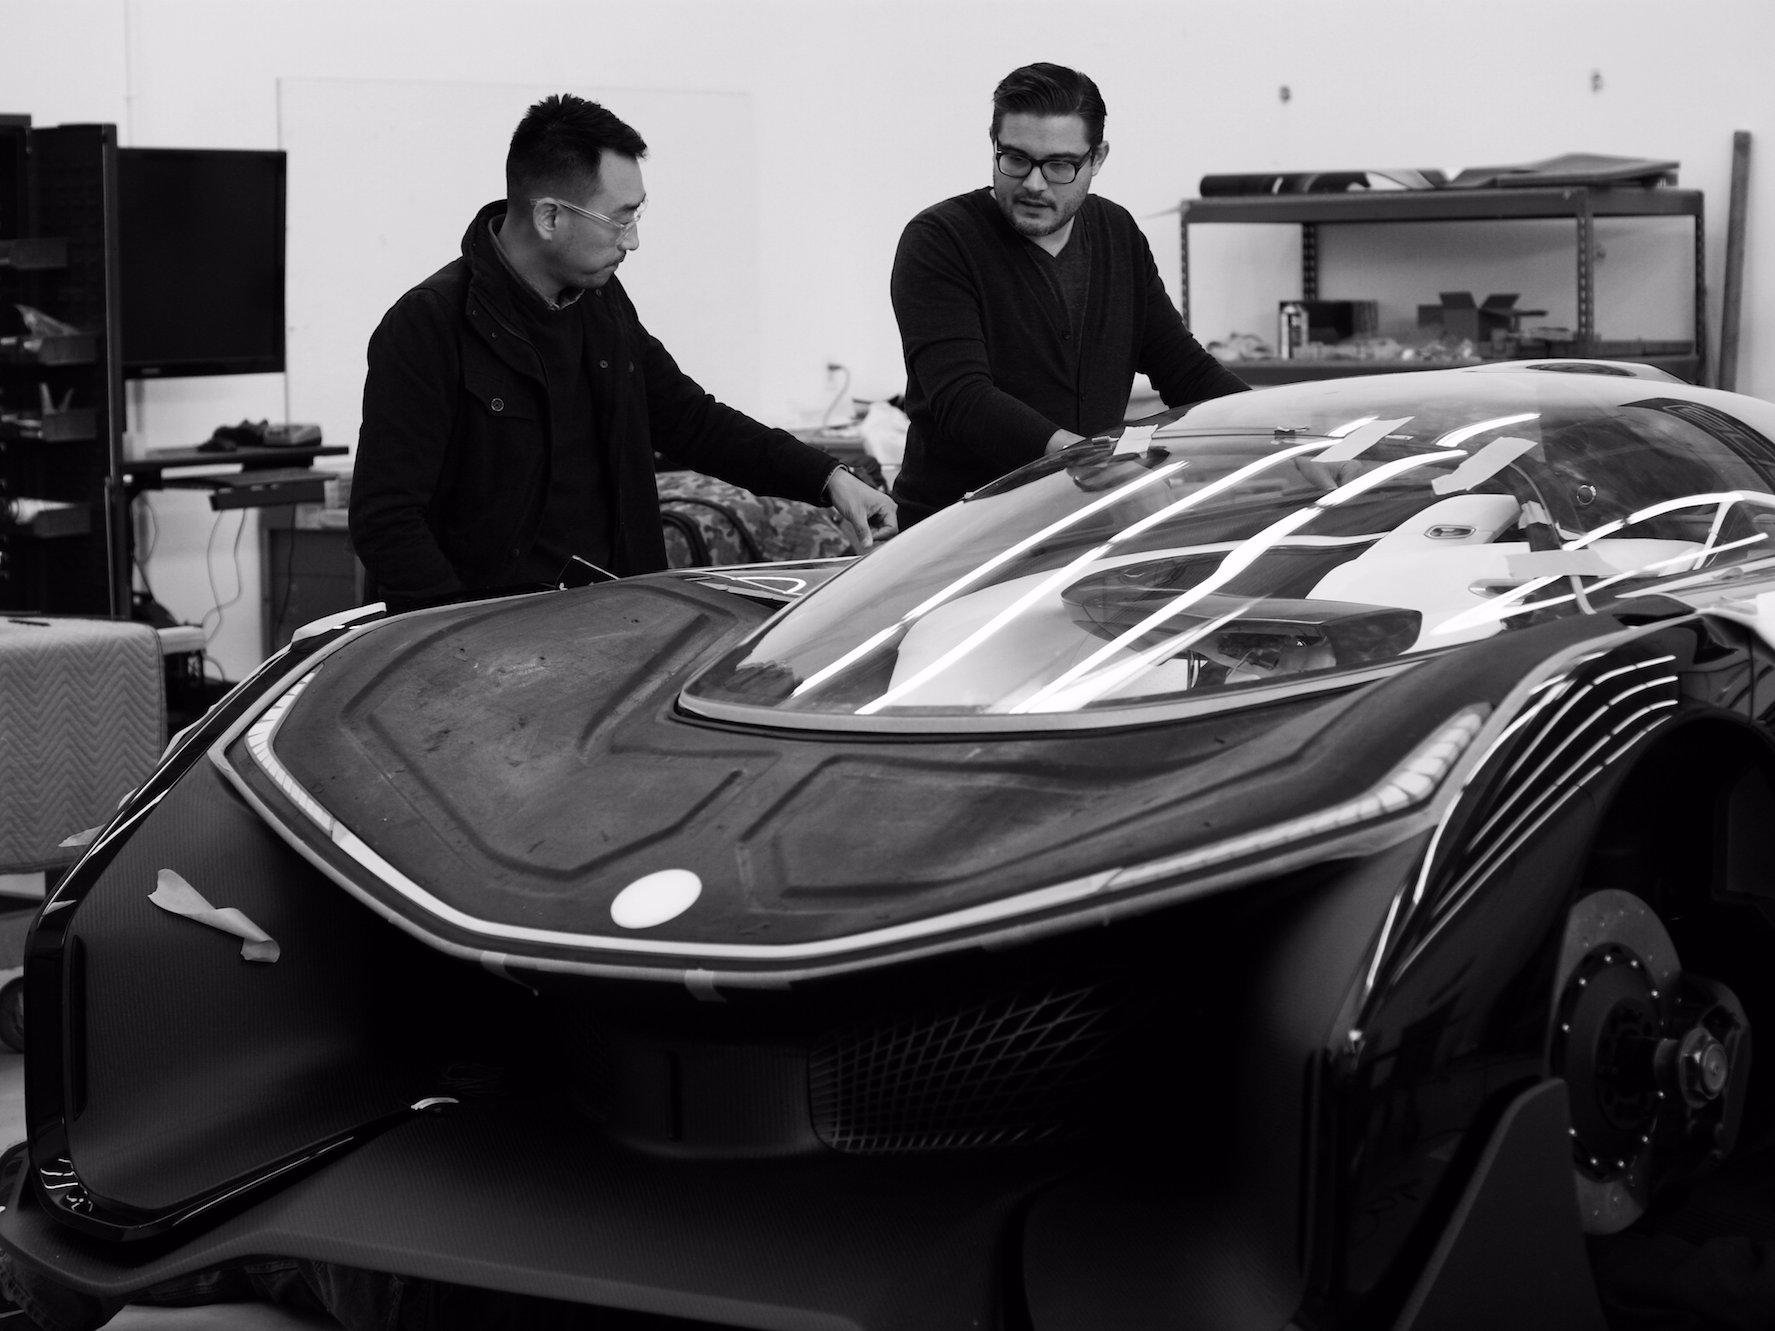
\includegraphics[width=\linewidth]{ffzero.jpg}
  \caption{\textit{Faraday Future} engineers prototyping the FFZERO in 2016  }
  \label{fig:marginfig}
\end{marginfigure}


\section{Electromotive Force}
Electromotive force, or emf, is denoted $\mathcal{E} $.  It is the voltage developed through a conducting circuit by a battery or dynamo.  It is not a force but an integral of the electric field over the current path.  It is similar to a voltage difference but may be non-zero over a closed path. 

\section{Motional Emf}
Consider a conducting bar of length $l$ moving perpendicularly through a magnetic field.  The charge carriers in the conductor undergo a magnetic force.  

$$\overrightarrow{F}_{B}=q\overrightarrow{v}\times \overrightarrow{B}$$

The conductor will polarize as the charge carriers move up until the point equilibrium is reached.  The effect is that an electric potential difference is maintained between the ends of a conductor moved perpendicularly through a magnetic field.  To determine the magnitude of this potential begin by equating the magnetic force and the electrostatic force.
$$F_E=F_B$$
$$qE=qvB \hspace{2cm} E=vB$$
Once the strength of the electric field is determined a potential difference is derived.
$$\Delta V=El=Blv$$

\newpage
\begin{marginfigure}[10pt]%
  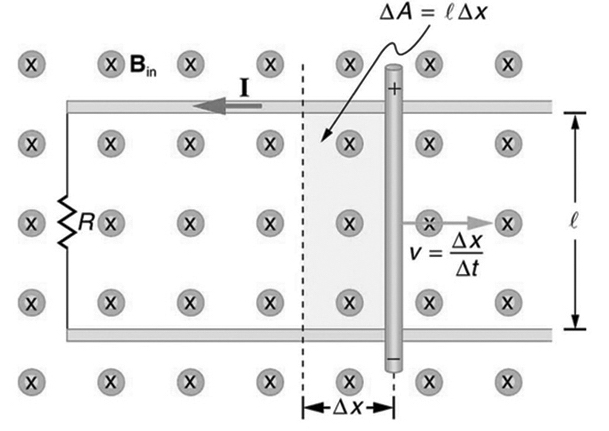
\includegraphics[width=\linewidth]{motional.jpeg}
  \caption{Motional emf}
  \label{fig:marginfig}
\end{marginfigure}
\noindent Now consider when the conducting bar is made part of a closed circuit with resistance $R$. In this case charge is free to flow through the circuit.  The bar is at position $x$.  The magnetic flux is determined as follows.
$$\Phi_B=Blx$$
The motional emf is determined.  
$$ \mathcal{E}=-\frac{d\Phi_B}{dt}=-Blv$$



\subsection{Power}
The power dissipated by the circuit is determined as follows.  Find the mechanical power.
$$P=Fv=IlBv=\frac{B^2l^2v^2}{R}$$
Find the electrical power. 
$$P=\frac{V^2}{R}=\frac{\mathcal{E}^2}{R}=\frac{B^2l^2v^2}{R}$$
Note their equivalence.


\section{Faraday's Law}
\begin{marginfigure}[150pt]%
  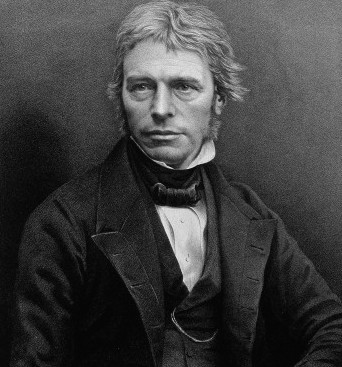
\includegraphics[width=\linewidth]{faraday.jpg}
  \caption{Michael Faraday}
  \label{fig:marginfig}
\end{marginfigure}

An emf is induced in a circuit by a changing magnetic field either by changing the area, relative orientation or strength of the magnetic field.  The induced emf is directly proportional to the time rate of change of the magnetic flux through the circuit.
$$ \mathcal{E}=-\frac{\Delta\Phi_B}{\Delta t} \hspace{2cm} \Phi_B=\sum\overrightarrow{B}\cdot \Delta\overrightarrow{A}$$
And for a circuit with $N$ coil loops.
$$ \mathcal{E}=-N\frac{\Delta\Phi_B}{\Delta t}$$



\section{Lenz's Law}
The induced emf produces a current which creates magnetic flux opposite the change of magnetic flux through the loop.\\ 

There are many ways to do this bookkeeping.  One way is to use a left hand rule.

\section{Induced Emf and Electric Field}
An electric field is generated in the conductor as a result of the changing magnetic flux.  In fact, an electric field is always generated by a changing magnetic flux, even in free space.
$$\sum_{\text{\tiny boundary}}\overrightarrow{E}\cdot \Delta\overrightarrow{s}=-\frac{\Delta\Phi_B}{\Delta t}$$


\section{Inductance}
\marginnote[-30pt]{
\subsection{Unit}
The unit for inductance is the Henry.  It is defined as the Volt second per Ampere.
$$1 \ \text{Henry}=\frac{1\ \text{Volt second}}{1\ \text{Ampere}}$$}
The term inductance was coined by Oliver Heaviside in 1886.  It is the property of an electrical conductor by which a change in current flowing through it induces an electromotive force in both the conductor itself (self-inductance) and in nearby conductors (mutual inductance).
$$ \mathcal{E}_L=-N\frac{\Delta\Phi_B}{\Delta t}=-L\frac{\Delta I}{\Delta t}$$
$$L=\frac{N\Phi_B}{I}$$



\section{RL Circuits}
\marginnote[0pt]{A simple RL circuit consists of a resistor and inductor in series with a battery.  The example circuit has a open switch that is closed at time $t=0$.  The resulting current approaches a constant value asymptotically.\\
Without the battery the circuit may be perturbed by giving the inductor a pulse of magnetic field.  In this case the current will decay exponentially.}
$$\begin{circuitikz} 
\draw
(0,0) to[battery] (4,0) to[closing switch] (4,2)
      to[resistor, l=$R$] (2,2) to[inductor, l=$L$] (0,2) -- (0,0);
\end{circuitikz}
$$
$$ \mathcal{E}=IR+L\frac{\Delta I}{\Delta t}$$
$$I(t)=\frac{\mathcal{E}}{R}\left(1-e^{-\frac{R}{L}t}\right)$$
%\vspace{1cm}

\section{LC Circuits}
\marginnote[0pt]{A simple LC circuit consists of a capacitor and inductor in series.  The example circuit begins with the capacitor charged and has a open switch that is closed at time $t=0$.  The resulting current is a sinusoidal oscillation.\\
Without the capacitor initially charged the circuit may be perturbed by giving the inductor a pulse of magnetic field.}
$$\begin{circuitikz} 
\draw
(0,0) -- (4,0) to[closing switch] (4,2)
      to[capacitor, l=$C$] (2,2) to[inductor, l=$L$] (0,2) -- (0,0);
\end{circuitikz}
$$
$$ 0=\frac{Q}{C}+L\frac{\Delta I}{\Delta t}$$
$$Q(t)=Q_0 \cos\left(\frac{t}{\sqrt{LC}}\right)$$
$$I(t)=-\frac{Q_0}{\sqrt{LC}} \sin\left(\frac{t}{\sqrt{LC}}\right)$$
%\vspace{1cm}
\section{Inductor Energy}
Consider the power dissipated in a RL circuit.
$$P=I \mathcal{E}=I^2R+LI\frac{\Delta I}{\Delta t}$$
The term representing the rate of change of energy stored in the magnetic field is shown below. 
$$\frac{\Delta U_B}{\Delta t}=LI\frac{\Delta I}{\Delta t}$$
The energy stored in the magnetic field is written as follows.
$$U_B=\frac{LI^2}{2}$$


\section{Maxwell's Equations}

\vspace{1cm}
\subsection{Gauss's Law}

$$\sum_{\text{\tiny boundary}}\overrightarrow{E}\cdot \Delta\overrightarrow{A}=\frac{q_{enc}}{\epsilon_0}$$

\vspace{1cm}
\subsection{Gauss's Law for Magnetism}

$$\sum_{\text{\tiny boundary}}\overrightarrow{B}\cdot \Delta\overrightarrow{A}=0$$

\vspace{1cm}
\subsection{Ampere-Maxwell Law}

$$\sum_{\text{\tiny boundary}}\overrightarrow{B}\cdot \Delta\overrightarrow{s}=\mu_0 I+\mu_0\epsilon_0\frac{\Delta\Phi_E}{\Delta t}$$

\vspace{1cm}
\subsection{Faraday's Law}

$$\sum_{\text{\tiny boundary}}\overrightarrow{E}\cdot \Delta\overrightarrow{s}=-\frac{\Delta\Phi_B}{\Delta t}$$
\chapter{Electromagnetic Waves}

\textit{When I talk about the fields swishing through space, I have a terrible confusion between the symbols I use to describe the objects and the objects themselves.}\\
\noindent\textbf{-   Richard Feynmann}

\vspace{1cm}

\begin{marginfigure}%
  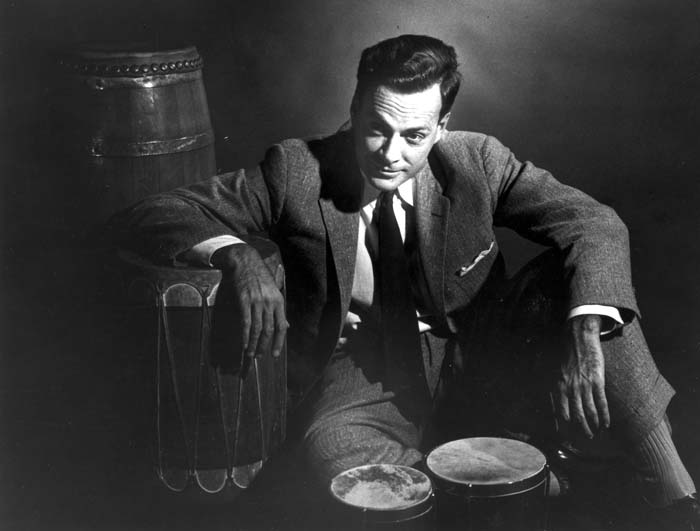
\includegraphics[width=\linewidth]{feynman.jpg}
  \caption{Richard Feynman with his bongos}
  \label{fig:marginfig}
\end{marginfigure}

\noindent Electromagnetic waves are synchronized oscillations of electric and magnetic fields.   They propagate at the speed of light through a vacuum.  The oscillations of the two fields are perpendicular to each other and perpendicular to the direction of energy and wave propagation.  The following analysis will derive the existence of electromagnetic waves in empty space.
\marginnote[30pt]{Electromagnetic waves are produced whenever charged particles are accelerated, and these waves can subsequently interact with any charged particles. They carry energy, momentum and angular momentum away from their source particle and can impart those quantities to matter with which they interact. }


\section{Gradient Operator (Grad or Del)}
The gradient operator is a vector whose components evaluate the slope (spatial rate of change) in the x, y and z directions respectively.
$$\nabla=\lim_{\Delta \rightarrow 0}\left[\begin{array}{c} \nicefrac{\Delta }{\Delta x} \\ \nicefrac{\Delta }{\Delta y} \\ \nicefrac{\Delta }{\Delta z}\end{array}\right]=\left[\begin{array}{c} \nicefrac{d }{d x} \\ \nicefrac{d }{d y} \\ \nicefrac{d}{d z}\end{array}\right]$$


\section{Divergence Theorem (Div)}
The divergence is the gradient operator dotted into a vector.  A vector field will have a different value for the divergence at every point in space.  The divergence is a scalar quantity representing how much a field emanates from a point in space.  \\
\marginnote[0pt]{$$\nabla \cdot \overrightarrow{E}=\left[\begin{array}{c} \nicefrac{dE_x }{d x} \\ \nicefrac{dE_y }{d y} \\ \nicefrac{dE_z}{d z}\end{array}\right]$$}
The divergence theorem states that the sum of the divergence of a vector field from all points is equal to the flux of the field through the bounding surface.  In other words, the total emanation of a field in a volume of space is equal to the  emanation through the surface of the volume.
$$\oint \overrightarrow{E} \cdot d\overrightarrow{A}=\int \nabla \cdot \overrightarrow{E} \ dV$$

\section{Stoke's Theorem (Curl)}
The curl is the gradient operator crossed into a vector.  A vector field will have a different curl at every point in space.  The curl is a vector quantity representing the circulation occuring at a point in space. 
\marginnote[0pt]{$$\nabla \times \overrightarrow{E}=\left[\begin{array}{c} \nicefrac{dE_z }{d y}-\nicefrac{dE_y }{d z} \\ \nicefrac{dE_x }{d z} -\nicefrac{dE_z }{d x}\\ \nicefrac{dE_y}{d x}-\nicefrac{dE_x }{d y}\end{array}\right]$$}
Stoke's theorem states that the sum of the curl for all points over a surface is equal to the sum of the field directed along the path bounin the surface.  In other words, the total circulation of a field over a surface is equal to the circulation along the perimeter of that area. 
$$\oint \overrightarrow{E} \cdot d\overrightarrow{s}=\int \nabla \times \overrightarrow{E} \cdot d\overrightarrow{A}$$

\section{Maxwell's Equations in Differential Form}
\begin{marginfigure}[100pt]
  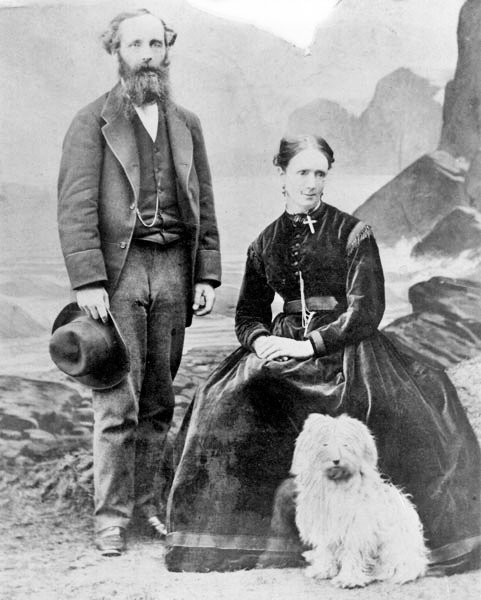
\includegraphics[width=\linewidth]{Maxwell_.jpg}
  \caption{James and Katherine Maxwell with their dog Fluffy McLovely}
  \label{fig:marginfig}
\end{marginfigure}
The mathematical derivation supporting the existence of electromagnetic fields in charge free space begins with expressing Maxwell's equations in differential form.

\subsection{Gauss's Law}
Gauss's law states that the electric flux through the surface of a volume of space is proportional to the amount of charge within that volume.  
$$\oint\overrightarrow{E}\cdot d\overrightarrow{A}=\frac{q_{enc}}{\epsilon_0}$$
By invoking the divergence theorem and expressing the enclosed charge as a integral of the charge density over the volume we can express both side of the equation as volume integrals.
$$ \int \nabla \cdot \overrightarrow{E} \ dV=\int \frac{\rho(\overrightarrow{r})}{\epsilon_0} \ dV$$
Therefore the integrands must be equivalent.
$$\nabla \cdot \overrightarrow{E} =\frac{\rho(\overrightarrow{r})}{\epsilon_0}$$

\subsection{Gauss's Law for Magnetism}
The same approach may be applied to Gauss's law for magnetism.
$$\oint\overrightarrow{B}\cdot d\overrightarrow{A}=0 \hspace{2cm} \oint \nabla \cdot \overrightarrow{B} \ dV=0$$
$$\nabla \cdot \overrightarrow{B} =0$$
Since there is no magnetic charge the right hand side of the equation is zero.  In other words, magnetic fields have zero divergence.  Magnetic fields do not emanate.

\vspace{1cm}
\subsection{Faraday's Law}
Faraday's law explains magnetic induction.  It states that the emf voltage in a loop is equivalent to the time rate of change of the magnetic flux through that loop.  The emf voltage is expressed as the path integral of the electric field around the loop.
$$\oint\overrightarrow{E}\cdot d\overrightarrow{s}=-\frac{d\Phi_B}{dt} $$
The left hand side of the equation may be expressed as an integral over an area using Stoke's theorem.  The right hand side is expressed as an integral over the area by using the definition of magnetic flux.
$$ \int \nabla \times \overrightarrow{E} \cdot d\overrightarrow{A}=-\frac{d}{dt}\int \overrightarrow{B} \cdot d\overrightarrow{A}$$
Once both sides of the equation are expressed as integrals over areas then the integrands may be determined as equal.  Thus we arrive at the differential form of Faraday's law.
$$\nabla \times \overrightarrow{E} =  -\frac{d\overrightarrow{B}}{dt}  $$
The curl off the electric field is equal to the negative of the time rate of change of the magnetic field.

\vspace{1cm}
\subsection{Ampere-Maxwell Law}
Ampere's law states that the line integral of the magnetic field along the boundary of a surface is proportional to the sum of the current and displacement current through a surface bound by said path.  Here the displacement current is the effective current produced by time rate of change of electric field through the surface.
$$\oint\overrightarrow{B}\cdot d\overrightarrow{s}=\mu_0 I+\epsilon_0\mu_0\frac{d\Phi_E}{dt}$$
The left hand side of the equation is transformed into a surface integral of the curl of the magnetic field using Stoke's theorem.  Each term of the right hand side of the equation is also transformed into a surface integral.  The current term is the surface integral of the current density through the surface.  The displacement current term is transformed into the rate of change of the integral of the electric field through the surface.  This second term is further transformed as the surface integral of the time rate of change of the electric field through the surface.
$$ \oint \nabla \times \overrightarrow{B} \cdot d\overrightarrow{A}=\int\mu_0 \overrightarrow{J}\cdot d\overrightarrow{A}+\frac{d}{dt}\int\epsilon_0\mu_0 \overrightarrow{E}\cdot d\overrightarrow{A}$$
Once all terms is the equation are expressed as surface integrals the integrands may be equated to yield the differential form of Ampere's law.
$$\nabla \times \overrightarrow{B} = \mu_0 \overrightarrow{J} +\epsilon_0\mu_0\frac{d\overrightarrow{E}}{dt}  $$

\marginnote[-50pt]{
\noindent \textbf{Maxwell equations differential form:}
$$\nabla \cdot \overrightarrow{E} =\frac{\rho(\overrightarrow{r})}{\epsilon_0}$$
$$\nabla \cdot \overrightarrow{B} =0$$
$$\nabla \times \overrightarrow{E} =  -\frac{d\overrightarrow{B}}{dt}  $$
$$\nabla \times \overrightarrow{B} = \mu_0 \overrightarrow{J} +\epsilon_0\mu_0\frac{d\overrightarrow{E}}{dt}  $$
}
\section{Maxwell's Equations in Charge-Free Space}
Once the differential forms of the Maxwell equations are determined they are considered in charge free space.  In space with no charge the charge density $\rho$, and current density $\overrightarrow{J}$ are both zero.  This yields the four equations shown in the margin.
\marginnote{
\noindent \textbf{Maxwell equations differential form in space without charges:}
$$\nabla \cdot \overrightarrow{E} =0$$ 
$$\nabla \cdot \overrightarrow{B} =0$$
$$\nabla \times \overrightarrow{E} =  -\frac{d\overrightarrow{B}}{dt}  $$
$$ \nabla \times \overrightarrow{B} =\epsilon_0\mu_0\frac{d\overrightarrow{E}}{dt}  $$}
These equations state that the electric and magnetic field have zero divergence in charge free space.  Additionally they state that the curl of the electric field is proportional to the time rate of change of the magnetic field and the curl of the magnetic field is proportional to the time rate of change of the electric field.  Note the high degree of symmetry in this system of equations.\\
To proceed in making sense of these equations we take the third equation and take the curl of both sides.  
$$\nabla \times \left(\nabla \times \overrightarrow{E}\right) = \nabla \times\left( -\frac{d\overrightarrow{B}}{dt}\right)  $$
\marginnote[-50pt]{\subsection{Double Curl}
$$\nabla \times(\nabla \times \overrightarrow{E}) =\nabla (\nabla \cdot  \overrightarrow{E})-\nabla^2\overrightarrow{E}$$
The second term of this identity includes the operator $\nabla^2$.  This is known as the Laplacian operator.  It is a scalar operator.
$$\nabla^2=\nabla \cdot \nabla=\left[\begin{array}{c} \nicefrac{d }{d x} \\ \nicefrac{d }{d y} \\ \nicefrac{d}{d z}\end{array}\right] \cdot \left[\begin{array}{c} \nicefrac{d }{d x} \\ \nicefrac{d }{d y} \\ \nicefrac{d}{d z}\end{array}\right]$$
$$\nabla^2=\frac{d^2 }{d x^2}+\frac{d^2 }{d y^2}+\frac{d^2 }{d z^2}$$}
On the left hand side of the equation we confront the double curl.  The double curl is the curl of the curl.  Whoa.  Using the identity detailed in the margin the left hand side of the equation becomes tractable.  On the right hand side of the equation the order of applying the the curl and time derivative are reversed.
$$\nabla (\nabla \cdot  \overrightarrow{E})-\nabla^2\overrightarrow{E}= -\frac{d \left( \nabla \times\overrightarrow{B}\right) }{dt} $$
At this point things simplify greatly.  The first term on the left hand side of the equation is zero since the electric field has no divergence in charge free space.  The right hand side of the equation which includes the curl of the magnetic field may make use of the last of Maxwell's equations. 
$$-\nabla^2\overrightarrow{E}= -\frac{d \left( \epsilon_0\mu_0\frac{d\overrightarrow{E}}{dt}\right) }{dt}  $$
Finally the analysis arrives at the following equation which states that the spatial curvature of the field is proportional to 
$$\nabla^2\overrightarrow{E}= \epsilon_0\mu_0\frac{d^2 \overrightarrow{E} }{dt^2}  $$


\section{Wave Equations}
\marginnote[0pt]{\subsection{Scalar Wave Equation}
$$\nabla^2 u=\frac{1}{v^2}{\partial^2 u \over \partial t^2} $$
Solutions to the scalar wave equation are sinusoidal scalar waves with wave speed $v$.}
Performing a near identical set of operations on the magnetic field yields an equivalent equation for the magnetic field.  The two equations are listed below.
$$\nabla^2\overrightarrow{E}=\epsilon_0\mu_0\frac{d^2\overrightarrow{E}}{dt^2} $$
$$\nabla^2\overrightarrow{B}=\epsilon_0\mu_0\frac{d^2\overrightarrow{B}}{dt^2} $$
We recognize these as similar to the scalar wave equation except that they are vectors.

\section{1-D Wave Equation Solutions}
Consider the solution of the one dimensional wave propagating in the positive x-direction.  This is known as a plane wave because the wavefronts cover an infinitely large plane.  Clearly this is an idealization and not physically realizable.  The magnitude of the electric and magnetic components are given below.
$$E=E_{max} \cos(kx-\omega t)$$
$$B=B_{max} \cos(kx-\omega t)$$
The wave speed of the solution is the speed of light, $c$.
$$v=\frac{k}{\omega}=\lambda f=\frac{1}{\sqrt{\epsilon_0\mu_0}}=\frac{E_{max}}{B_{max}}=c$$
$$c=3.00\times 10^8 \frac{\text{meter}}{\text{second}}$$

\section{Poynting Vector}
The Poynting vector represents the rate of energy flow through a unit surface area perpendicular to the direction of wave propagation.  The Poynting vector points in the same direction that the wave propagates.


\begin{minipage}{7cm}

$$\overrightarrow{S} \equiv \frac{1}{\mu_0} \overrightarrow{E} \times \overrightarrow{B} $$
\end{minipage}
\begin{minipage}{7cm}
\tdplotsetmaincoords{60}{110}
$$\begin{tikzpicture}[scale=1,tdplot_main_coords]
\coordinate (O) at (0,0,0);
\coordinate (P) at (1,2,3);
\draw[very thick,->] (0,0,0) -- (2,0,0) node[anchor=north ]{$B$};
\draw[very thick,->] (0,0,0) -- (0,2,0) node[anchor= west]{$v,S$};
\draw[very thick,->] (0,0,0) -- (0,0,2) node[anchor=south]{$E$};
\end{tikzpicture}
$$
\end{minipage}

\section{Wave Energy}
The intensity of the wave is the power delivered by the wave per unit area.  This is the average value of the Poynting vector.
$$I=S_{av}=\frac{E_{max}B_{max}}{2\mu_0} \hspace{2cm} \frac{E}{B}=c$$
At any instant the energy stored per unit volume is $u$.  The energy per unit volume is split between the electric field and magnetic field evenly.  The electric energy per unit volume and magnetic energy per unit volume are $u_E$ and $u_B$ respectively.
$$u_E=\frac{\epsilon_0}{2}E^2 \hspace{2cm} u_B=\frac{1}{2\mu_0}B^2 \hspace{2cm} u_E=u_B$$
The time average energy per unit volume is half the total maximum energy per unit volume.
$$u=u_E+u_B \hspace{2cm} u_{av}=\frac{u_{max}}{2}$$
The intensity is the product of the speed of light and the average energy per unit volume.
$$I=S_{av}=cu_{av}$$

\section{Momentum and Radiation Pressure}
Electromagnetic radiation carries a volumetric momentum density and applies a radiation pressure when it impacts a surface.
\subsection{Complete Absorption}
When hitting a radiation absorber the impulse $\Delta p$to the surface is the wave energy, $U$, divided by its velocity, $c$.  The radiation pressure $P$ is the intensity divided by its speed.
$$\Delta p=\frac{U}{c} \hspace{2cm} P=\frac{S}{c}$$
\subsection{Complete Reflection}
In the case of a reflector the impulse and pressure are double.
$$\Delta p=\frac{2U}{c} \hspace{2cm} P=\frac{2S}{c}$$

\section{Polarization (Malus's Law)}
Light may have electric fields in any direction perpendicular to its direction of propagation.  Polarized light is light that has all of its electric field aligned in a single direction.  Filters may be used to align the polarization along a particular direction.
\subsection{Polarized Light}
When polarized light passed through a polarizing filter the intensity of the transmitted light is as follows.
$$I_{transmitted}=I_0\cos^2 \theta$$
\subsection{Unpolarized Light}
For unpolarized light traveling through a polarizing filter the following behavior is observed.
$$I_{transmitted}=\frac{I_0}{2}$$

\section{Spectrum of Electromagnetic Waves}
In free space the frequency of electromagnetic radiation completely determines its wavelength since the speed of light is constant.
$$c=f \lambda$$
Below is a diagram detailing various wavelengths of electromagnetic radiation.
\begin{center}
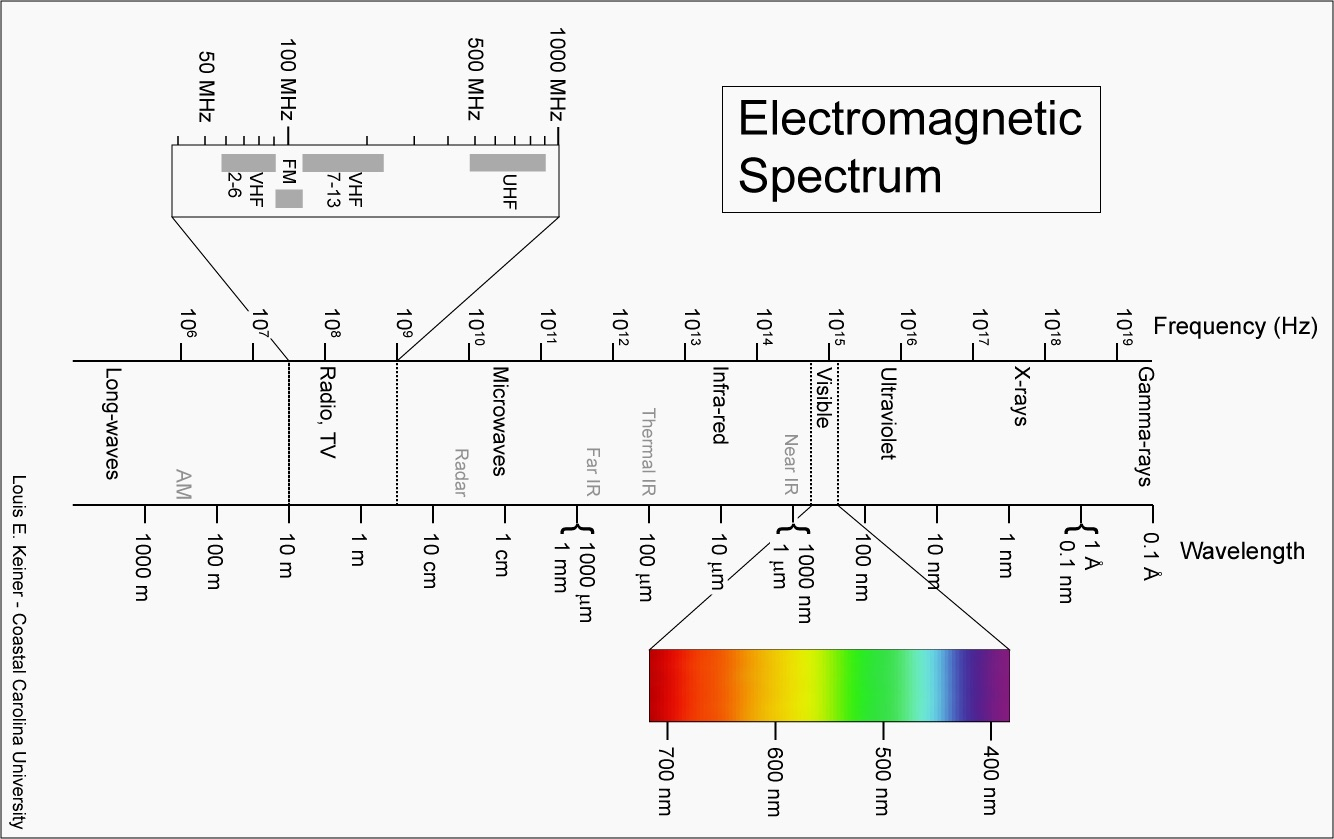
\includegraphics[height=4in,width=6in,angle=0]{spectrum.jpg}

\end{center}

\tikzstyle arrowstyle=[scale=1]
\tikzstyle directed=[postaction={decorate,decoration={markings,
    mark=at position .65 with {\arrow[arrowstyle]{stealth}}}}]
\tikzstyle reverse directed=[postaction={decorate,decoration={markings,
    mark=at position .65 with {\arrowreversed[arrowstyle]{stealth};}}}]

\chapter{Light \& Optics}

\textit{Music is the arithmetic of sounds as optics is the geometry of light.}\\
\noindent\textbf{-   Claude Debussy}

\vspace{0.5cm}


\begin{marginfigure}%
  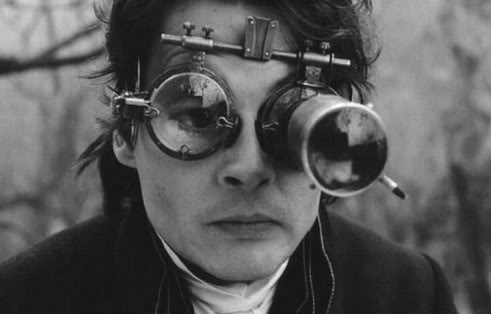
\includegraphics[width=\linewidth]{depp.jpg}
  \caption{Depp's optics (\textit{Sleepy Hollow})}
  \label{fig:marginfig}
\end{marginfigure}

Most optical phenomena can be accounted for using the classical electromagnetic description of light. Complete electromagnetic descriptions of light are, however, often difficult to apply in practice. Geometric optics, treats light as a collection of rays that travel in straight lines and bend when they pass through or reflect from surfaces. Diffraction and interference require a wave model of light and cannot be accounted using geometric optics.

\marginnote[-20pt]{\section{Light Rays}
A light ray is an idealized model of light, obtained by choosing a line that is perpendicular to the wavefronts of the actual light, and that points in the direction of energy flow.  Rays are used to model the propagation of light through an optical system, by dividing the real light field up into discrete rays and tracked through ray tracing.  
\subsection{Ray Angle}
At an interface, ray angles are described relative to the surface normal.}

\section{Refractive Index}
 The refractive index or index of refraction $n$ of a material is a dimensionless number that describes how light propagates through that medium. It is defined as the ratio between the speed of light through vacuum and the speed of light through that material.
 
 $$n=\frac{c}{v}$$

\section{Reflection, Refraction \& Snell's Law}
\begin{marginfigure}[20pt]
  \begin{tikzpicture}[scale=0.65]

    % define coordinates
    \coordinate (O) at (0,0) ;
    \coordinate (A) at (0,4) ;
    \coordinate (B) at (0,-4) ;
    
    % media
    \fill[blue!25!,opacity=.3] (-4,0) rectangle (4,4);
    \fill[blue!60!,opacity=.3] (-4,0) rectangle (4,-4);
    \node[right] at (2,2) {Air, $n_1$};
    \node[left] at (-1.5,-2) {Water, $n_2$};

    % axis
    \draw[dash pattern=on5pt off3pt] (A) -- (B) ;

    % rays
    \draw[red,ultra thick,reverse directed] (O) -- (130:5.2);
     \draw[red,ultra thick, directed] (O)--(-130:-5.2) ;
    \draw[blue,directed,ultra thick] (O) -- (-70:4.24);

    % angles
    \draw (0,1) arc (90:130:1);
     \draw (0,1) arc (90:50:1);
    \draw (0,-1.4) arc (270:290:1.4) ;
    \node[] at (280:1.8)  {$\theta_{2}$};
    \node[] at (110:1.4)  {$\theta_{1}$};
      \node[] at (-110:-1.4)  {$\theta_{1}$};
\end{tikzpicture}
  \caption{Reflection and refraction}
  \label{fig:marginfig}
\end{marginfigure}
\textbf{Reflection} is the change in direction of a wavefront at an interface between two different media so that the wavefront returns into the medium from which it originated. For specular reflection the incident ray angle equals reflected ray angle.
$$\theta_{incidence}=\theta_{reflection} $$
\textbf{Refraction} is the change in direction of propagation of a wave due to a change in its transmission medium.  \textbf{Snell's law} describes the relationship between the angle of the incident ray and that of the refracted ray.

$$n_1\sin\theta_1=n_2\sin\theta_2$$

Snell's law may be derived in various ways.  One way is to match the frequency of the incident and refracted wave at the surface.
\marginnote[-20pt]{\section{Fermat's Principle} 
Fermat's principle states that when light travels between any two points its path is the one that requires the least time.  Snell's law may also be derived from this principle.  In truth it is less of a principle and more of a feature of light and refraction.}
$$f_1=f_2$$
Representing the frequency as a ratio of the velocity and the wavelength yields the following.
$$ \frac{v_1}{\lambda_1}= \frac{v_2}{\lambda_2}$$
Substituting the velocity as the ratio of the speed of light and the index of refraction gives the following.
$$ \frac{c}{n_1\lambda_1}= \frac{c}{n_2\lambda_2}$$
This simplifies further.
$$n_1 \lambda_1 =n_2 \lambda_2 $$
The distance between wave peaks along the interface is $d$.  It must be the same value on both sides of the interface.  Representing the wavelength in terms of $d$ gives the following.
\begin{marginfigure}%
  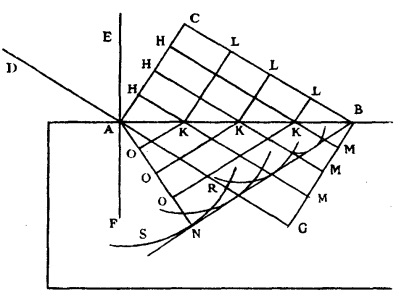
\includegraphics[width=\linewidth]{Huygens_construction.jpg}
  \caption{Huygens' construction}
  \label{fig:marginfig}
\end{marginfigure}
$$n_1 d \sin \theta_1=n_2 d \sin \theta_2$$
Finally cancelling $d$ yields Snell's law. 
$$n_1  \sin \theta_1=n_2  \sin \theta_2$$

\section{Total Internal Reflection}
\begin{marginfigure}[40pt]
  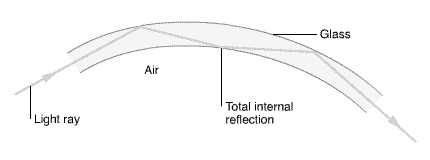
\includegraphics[width=\linewidth]{tir.jpg}
  \caption{Total internal reflection in a fiber optic cable}
  \label{fig:marginfig}
\end{marginfigure}
Total internal reflection is a limiting case of refraction.  In the case of total internal reflection the refracted angle is 90 degrees, namely there is no refracted ray.
$$n_1\sin\theta_c=n_2\sin 90$$
The critical angle for total internal reflection is given as follows.
$$\theta_c=\sin^{-1}\left(\frac{n_2}{n_1}\right)$$
This is possible when light is passing from a medium of higher refractive index to lower refractive index.

\newpage

\section{Dispersion}
\begin{marginfigure}[0pt]
  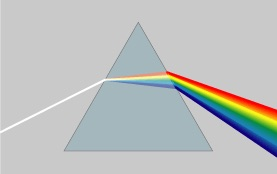
\includegraphics[width=\linewidth]{prism.jpg}
  \caption{Dispersion of white light through a prism}
  \label{fig:marginfig}
\end{marginfigure}

In many wave-propagation media, wave velocity changes with frequency or wavelength of the waves; this is true of light propagation in most transparent substances other than a vacuum. These media are called dispersive. The result is that the angles determined by Snell's law also depend on frequency or wavelength, so that a ray of mixed wavelengths, such as white light, will spread or disperse. Such dispersion of light in glass or water underlies the origin of rainbows and other optical phenomena, in which different wavelengths appear as different colors.  In short, indices of refraction are wavelength dependent.

\subsection{Rainbows}
\begin{marginfigure}[50pt]
  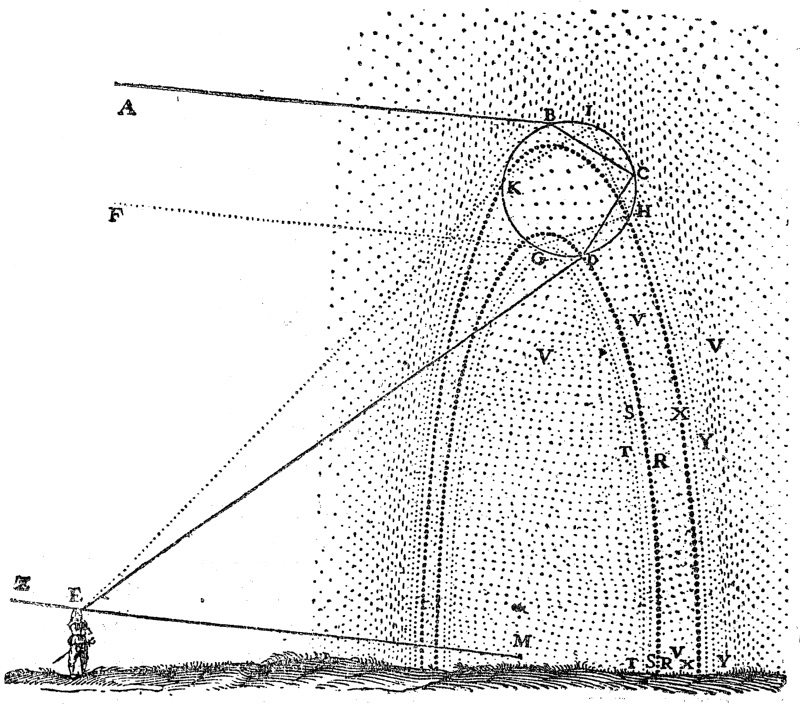
\includegraphics[width=\linewidth]{Descartes_Rainbow.jpg}
  \caption{Descartes diagram of rainbow formation}
  \label{fig:marginfig}
\end{marginfigure}
A rainbow is a meteorological phenomenon that is caused by reflection, refraction and dispersion of light in water droplets resulting in a spectrum of light appearing in the sky. It takes the form of a multicoloured arc. Rainbows caused by sunlight always appear in the section of sky directly opposite the sun.\\
The following diagram shows how rainbows for through light refraction-reflection-refraction interaction with a water droplet.
\vspace{1.5cm}

\begin{figure*}[htbp]
\centering
% Draw an arc denoting an angle using start and delta angles
\newcommand{\drawarcdelta}[4]{
  \draw ($#1+(#2:#4)$) arc[start angle=#2, delta angle=#3, radius=#4];
}

% Draw an arc with label denoting an angle using start and delta angles
\newcommand{\drawlabeledarcdelta}[6]{
  \drawarcdelta{#1}{#2}{#3}{#4}
  \node at ($#1+(#2+#3/2:#6)$) {#5};
}


\begin{tikzpicture}[xscale=-0.8,yscale=0.8,
    ray/.style={decoration={markings,mark=at position .5 with {
      \arrow[>=latex]{>}}},postaction=decorate}
  ]

  % Radius of raindrop
  \pgfmathsetlengthmacro{\r}{3cm}
  % Position where the incoming ray enters the raindrop, as a fraction of
  % the height of the drop.  If 0., the ray will enter in the middle of the
  % drop, if 1., the ray will enter at the top of the drop.
  \pgfmathsetmacro{\f}{.7}

  % Various radii for drawing angle arcs and labels
  \pgfmathsetlengthmacro{\arcradius}{.8cm}
  \pgfmathsetlengthmacro{\dotradius}{.6cm}
  \pgfmathsetlengthmacro{\arclabelradius}{1cm}

  % Calculation of the angle of incidence
  \pgfmathsetmacro{\incidentangle}{asin(\f)}

  % Coordinates of origin and point of entry
  \coordinate (O) at (0, 0);
  \coordinate (A) at (\incidentangle:\r);

  % Draw the drop and the incoming ray, as well as the angle of incidence
  \draw (O) circle (\r);
  \draw[ray] (A  -| \r*3, 0) -- (A);
  \draw[gray] (O) -- ($(O)!1.5!(A)$) node[pos=1.05] {$n$};
  \drawarcdelta{(A)}{0}{\incidentangle}{\arcradius-1pt}
  \drawlabeledarcdelta{(A)}{0}{\incidentangle}{\arcradius+1pt}
    {$i$}{\arclabelradius}

  % For each red and blue ray.  The index of refraction for red light is
  % slightly exaggerated, it should be 1.33.
  \foreach \index/\color in {1.32/red, 1.34/blue} {
    % Calculate angle of refraction
    \pgfmathsetmacro{\refractedangle}{asin(sin(\incidentangle) / \index)}
    % Calculate top angle (at O) in the triangle formed by O, the point of
    % entry, and the point of internal reflection
    \pgfmathsetmacro{\angleindrop}{180 - 2*\refractedangle}

    % Coordinate of point of reflection
    \coordinate (A') at (\incidentangle+\angleindrop:\r);
    % Coordinate of point of exit
    \coordinate (A'') at (\incidentangle+2*\angleindrop:\r);

    \begin{scope}[opacity=.5, color=\color]
      % Draw the light rays
      \draw[ray] (A) -- (A');
      \draw[ray] (A') -- (A'');
      \draw[ray] (A'') -- ($(A'')+(2*\incidentangle+2*\angleindrop:2*\r)$);

      % Draw the normal lines
      \draw (O) -- ($(O)!1.5!(A')$) node[pos=1.05] {$n$};
      \draw (O) -- ($(O)!1.5!(A'')$) node[pos=1.05] {$n$};

      % Draw the arcs and labels
      \drawlabeledarcdelta{(A)}{\incidentangle+180}{-\refractedangle}
        {\arcradius}{$r$}{\arclabelradius}
      \drawarcdelta{(A')}{\incidentangle+\angleindrop+180}{\refractedangle}
        {\arcradius}
      \drawarcdelta{(A')}{\incidentangle+\angleindrop+180}{-\refractedangle}
        {\arcradius}
      \drawarcdelta{(A'')}{\incidentangle+2*\angleindrop+180}{\refractedangle}
        {\arcradius}
    \end{scope}

    % Draw the arcs of the angles of the rays leaving the raindrop.  Note
    % that the angles are identical to the original angle of incidence.
    \drawarcdelta{(A'')}{\incidentangle+2*\angleindrop}{\incidentangle}
      {\arcradius-1pt}
    \drawarcdelta{(A'')}{\incidentangle+2*\angleindrop}{\incidentangle}
      {\arcradius+1pt}
  }

  % Mark the center of the raindrop
  \draw[fill] (O) circle (1.5pt);
\end{tikzpicture}
\caption{Raindrop producing a rainbow}
  \label{fig:GreyScaleSimilarity}
\end{figure*}
\newpage



\section{Geometric Optics}
Geometric optics uses ray tracing to model light. 

\marginnote[-50pt]{
\subsection{Thin Lens Equation}
Light's interaction with thin lenses can be modeled using the thin lens equation.  Here $f$ is the focal length, $d_i$ is the distance from the lens to image and $d_o$ is the distance from the lens to the object.
$$\frac{1}{f}=\frac{1}{d_i}+\frac{1}{d_o}$$
}
\section{Convergent/Convex Lenses (f>0)}
As light rays parallel to the optical axis hit a convergent lens they are scattered to pass through the focus.  The rays converge on the focal point.  Convex lenses are convergent.  \\
\begin{figure*}[htbp]
\centering

\begin{tikzpicture}[scale=0.8]

\filldraw[fill=green!20!white, draw=green!50!black] 
(-0.3,-2.5) -- (0.3,-2.5) arc (-9.148:9.148:15.725) -- (-0.3,2.5) arc (170.852:189.148:15.725);

\draw [color=black!30] (8,-2) -- (8,2);

\draw (-10,0) -- (10,0);
\draw [color=gray] (0,-2.6) -- (0,2.6);

\draw [color=red!50] (-10,1) -- (0,1);
\draw [color=red!50] (-10,2) -- (0,2);
\draw [color=red!50] (-10,-1) -- (0,-1);
\draw [color=red!50] (-10,-2) -- (0,-2);

\draw [color=red!50]  (0,1) -- (10,-1.5);
\draw [color=red!50]  (0,2) -- (10,-3);
\draw [color=red!50] (0,-1) -- (10,1.5);
\draw [color=red!50] (0,-2) -- (10,3);

\fill (4,0) circle (0.1);
\draw (4,0) node [anchor=north,scale=1.5] {$f$};
\fill (8,0) circle (0.1);
\draw (8,0) node [anchor=north,scale=1.5] {$2f$};


\end{tikzpicture}

 \caption{Convergent Lens}
  \label{fig:GreyScaleSimilarity}
\end{figure*}
\marginnote[0pt]{
\subsection{Magnification}
Magnification is the ratio of the height of the focused image $h_i$ to the height of the light emitting object $h_o$.
$$M=\frac{h_i}{h_o}=-\frac{d_i}{d_o}$$}
A light emitting object with a $d_0$ greater that $2f$ will produce an image with a $d_i$ between $f$ and $2f$.  The magnification in this case is negative and has a magnitude which is less than one.
\vspace{2cm}

\begin{figure*}[htbp]
\centering

\begin{tikzpicture}[scale=0.8]

\filldraw[fill=green!20!white, draw=green!50!black] 
(-0.3,-2.5) -- (0.3,-2.5) arc (-9.148:9.148:15.725) -- (-0.3,2.5) arc (170.852:189.148:15.725);

%\draw [color=black!30] (8,-2) -- (8,2);

\draw (-10,0) -- (10,0);
\draw [color=gray] (0,-2.6) -- (0,2.6);


\draw [color=red!50] (-9,2) -- (0,2);
\draw [color=red!50] (-9,2) -- (10,-2.222);
\draw [color=red!50] (-9,2) -- (0,-1.6);
\draw [color=red!50] (0,-1.6) -- (10,-1.6);

\draw [color=red!50]  (0,2) -- (10,-3);


\draw [->, color=blue, line width = 1mm] (-9,0) -- (-9,2);

\draw [->, color=blue, line width = 1mm] (7.2,0) -- (7.2,-1.6);

\fill [color=blue] (-9,0) circle (0.1);
\fill [color=blue] (7.2,0) circle (0.1);


\fill (4,0) circle (0.1);
\draw (4,0) node [anchor=north,scale=1.5] {$f$};
\fill (8,0) circle (0.1);
\draw (8,0) node [anchor=north,scale=1.5] {$2f$};


\fill (-4,0) circle (0.1);
\draw (-4,0) node [anchor=north,scale=1.5] {$f$};
\fill (-8,0) circle (0.1);
\draw (-8,0) node [anchor=north,scale=1.5] {$2f$};
\draw (-9,0) node [anchor=north,scale=1.5] {$d_o$};
\draw (-9,1) node [anchor=east,scale=1.5] {$h_o$};
\draw (7.2,0) node [anchor=south,scale=1.5] {$d_i$};
\draw (7.2,-0.8) node [anchor=east,scale=1.5] {$h_i$};



\end{tikzpicture}

 \caption{$d_0>2f$}
  \label{fig:GreyScaleSimilarity}
\end{figure*}

A light emitting object with a $d_0$ equal $2f$ will produce an image with a $d_i$ equal to $2f$.  The magnification in this case is negative one.
 \newpage

\begin{figure*}[htbp]
\centering

\begin{tikzpicture}[scale=0.8]

\filldraw[fill=green!20!white, draw=green!50!black] 
(-0.3,-2.5) -- (0.3,-2.5) arc (-9.148:9.148:15.725) -- (-0.3,2.5) arc (170.852:189.148:15.725);

%\draw [color=black!30] (8,-2) -- (8,2);

\draw (-10,0) -- (10,0);
\draw [color=gray] (0,-2.6) -- (0,2.6);


\draw [color=red!50] (-8,2) -- (0,2);
\draw [color=red!50] (-8,2) -- (10,-2.5);
\draw [color=red!50] (-8,2) -- (0,-2);
\draw [color=red!50] (0,-2) -- (10,-2);

\draw [color=red!50]  (0,2) -- (10,-3);


\draw [->, color=blue, line width = 1mm] (-8,0) -- (-8,2);

\draw [->, color=blue, line width = 1mm] (8,0) -- (8,-2);

\fill [color=blue] (-8,0) circle (0.1);
\fill [color=blue] (8,0) circle (0.1);


\fill (4,0) circle (0.1);
\draw (4,0) node [anchor=north,scale=1.5] {$f$};

\draw (8,0) node [anchor=south,scale=1.5] {$2f$};


\fill (-4,0) circle (0.1);
\draw (-4,0) node [anchor=north,scale=1.5] {$f$};

\draw (-8,0) node [anchor=north,scale=1.5] {$2f$};
%\draw (-9,0) node [anchor=north,scale=1.5] {$d_o$};
\draw (-8,1) node [anchor=east,scale=1.5] {$h$};
%\draw (8,0) node [anchor=south,scale=1.5] {$d_i$};
\draw (8,-0.8) node [anchor=west,scale=1.5] {$h$};



\end{tikzpicture}

 \caption{$d_0=2f$}
  \label{fig:GreyScaleSimilarity}
\end{figure*}
A light emitting object with a $d_0$ between $2f$ and $f$ will produce an image with a $d_i$ greater than $2f$.  The magnification in this case is negative and has a magnitude which is greater than one.

\begin{figure*}[htbp]
\centering

\begin{tikzpicture}[scale=0.8]

\filldraw[fill=green!20!white, draw=green!50!black] 
(-0.3,-2.5) -- (0.3,-2.5) arc (-9.148:9.148:15.725) -- (-0.3,2.5) arc (170.852:189.148:15.725);

%\draw [color=black!30] (8,-2) -- (8,2);

\draw (-10,0) -- (10,0);
\draw [color=gray] (0,-2.6) -- (0,2.6);


\draw [color=red!50] (-7.2,2) -- (0,2);
\draw [color=red!50] (-7.2,2) -- (10,-2.7777);
\draw [color=red!50] (-7.2,2) -- (0,-2.5);
\draw [color=red!50] (0,-2.5) -- (10,-2.5);

\draw [color=red!50]  (0,2) -- (10,-3);


\draw [->, color=blue, line width = 1mm] (-7.2,0) -- (-7.2,2);

\draw [->, color=blue, line width = 1mm] (9,0) -- (9,-2.5);

\fill [color=blue] (-7.2,0) circle (0.1);
\fill [color=blue] (9,0) circle (0.1);


\fill (4,0) circle (0.1);
\draw (4,0) node [anchor=north,scale=1.5] {$f$};
\fill (8,0) circle (0.1);
\draw (8,0) node [anchor=north,scale=1.5] {$2f$};


\fill (-4,0) circle (0.1);
\draw (-4,0) node [anchor=north,scale=1.5] {$f$};
\fill (-8,0) circle (0.1);
\draw (-8,0) node [anchor=north,scale=1.5] {$2f$};
\draw (-7.2,0) node [anchor=north,scale=1.5] {$d_o$};
\draw (-7.2,1) node [anchor=east,scale=1.5] {$h_o$};
\draw (9,0) node [anchor=south,scale=1.5] {$d_i$};
\draw (9,-1.25) node [anchor=west,scale=1.5] {$h_i$};



\end{tikzpicture}

 \caption{$2f>d_0>f$}
  \label{fig:GreyScaleSimilarity}
\end{figure*}

A light emitting object with a $d_0$ equal to $f$ will not produce an image since the rays transmitted through the lens will be parallel.  The image may be described as existing at infinity.

\begin{figure*}[htbp]
\centering

\begin{tikzpicture}[scale=0.8]

\filldraw[fill=green!20!white, draw=green!50!black] 
(-0.3,-2.5) -- (0.3,-2.5) arc (-9.148:9.148:15.725) -- (-0.3,2.5) arc (170.852:189.148:15.725);

%\draw [color=black!30] (8,-2) -- (8,2);

\draw (-10,0) -- (10,0);
\draw [color=gray] (0,-2.6) -- (0,2.6);


\draw [color=red!50] (-4,2) -- (0,2);
\draw [color=red!50] (-4,2) -- (6,-3);
%\draw [color=red!50] (-7.2,2) -- (0,-2.5);
%\draw [color=red!50] (0,-2.5) -- (10,-2.5);

\draw [color=red!50]  (0,2) -- (10,-3);


\draw [->, color=blue, line width = 1mm] (-4,0) -- (-4,2);

%\draw [->, color=blue, line width = 1mm] (9,0) -- (9,-2.5);


%\fill [color=blue] (9,0) circle (0.1);


\fill (4,0) circle (0.1);
\draw (4,0) node [anchor=north,scale=1.5] {$f$};
\fill (8,0) circle (0.1);
\draw (8,0) node [anchor=north,scale=1.5] {$2f$};


\fill [color=blue] (-4,0) circle (0.1);;
\draw (-4,0) node [anchor=north,scale=1.5] {$f$};
\fill (-8,0) circle (0.1);
\draw (-8,0) node [anchor=north,scale=1.5] {$2f$};
%\draw (-7.2,0) node [anchor=north,scale=1.5] {$d_o$};
%\draw (-7.2,1) node [anchor=east,scale=1.5] {$h_o$};
%\draw (9,0) node [anchor=south,scale=1.5] {$d_i$};
%\draw (9,-1.25) node [anchor=west,scale=1.5] {$h_i$};



\end{tikzpicture}

 \caption{$d_0=f$}
  \label{fig:GreyScaleSimilarity}
\end{figure*}

A light emitting object with a $d_0$ less than $f$ will not produce an image since the rays transmitted through the lens will diverge.  The image may be described as existing with a $d_i$ that is negative.  The image does not exist.  It is virtual.  The magnification is positive and greater than one.

\newpage

\begin{figure*}[htbp]
\centering

\begin{tikzpicture}[scale=0.8]

\filldraw[fill=green!20!white, draw=green!50!black] 
(-0.3,-2.5) -- (0.3,-2.5) arc (-9.148:9.148:15.725) -- (-0.3,2.5) arc (170.852:189.148:15.725);

%\draw [color=black!30] (8,-2) -- (8,2);

\draw (-10,0) -- (10,0);
\draw [color=gray] (0,-2.6) -- (0,2.6);


\draw [color=red!50] (-2,2) -- (0,2);
\draw [color=red!50] (-2,2) -- (2.5,-2.5);



\draw [color=red!50]  (0,2) -- (10,-3);


\draw [->, color=blue, line width = 1mm] (-2,0) -- (-2,2);

\draw [->, dotted, color=blue, line width = 1mm] (-4,0) -- (-4,4);

\fill [color=blue] (-2,0) circle (0.1);
\fill [color=blue] (-4,0) circle (0.1);


\fill (4,0) circle (0.1);
\draw (4,0) node [anchor=north,scale=1.5] {$f$};
\fill (8,0) circle (0.1);
\draw (8,0) node [anchor=north,scale=1.5] {$2f$};



\draw (-4,0) node [anchor=north,scale=1.5] {$f$};
\fill (-8,0) circle (0.1);
\draw (-8,0) node [anchor=north,scale=1.5] {$2f$};
\draw (-2,0) node [anchor=north,scale=1.5] {$f/2$};
\draw (-2,1) node [anchor=east,scale=1.5] {$h$};
%\draw (9,0) node [anchor=south,scale=1.5] {$d_i$};
\draw (-4,2) node [anchor=east,scale=1.5] {$2h$};

\draw [color=red!50,dashed]  (0,2) -- (-4,4);
\draw [color=red!50,dashed]  (-2,2) -- (-4,4);

\end{tikzpicture}

 \caption{$d_0<f$}
  \label{fig:GreyScaleSimilarity}
\end{figure*}


\section{Divergent/Concave Lenses (f<0)}
As light rays parallel to the optical axis hit a divergent lens they are scattered away from the optical axis and do not converge at a point.  Geometrically they diverge as if they come from a point on the other side of the lens.  This point is the focal point of a divergent lens.  The focal length of a divergent lens is negative.  Concave lenses are divergent.

\begin{figure*}[htbp]
\centering

\begin{tikzpicture}[scale=0.7]

\filldraw[fill=green!20!white, draw=green!50!black] 
(-0.3,-2.5) -- (0.3,-2.5) arc (189.148:170.852:15.725) -- (-0.3,2.5) arc (9.148:-9.148:15.725);
\draw [color=black!30] (-8,-2) -- (-8,2);
\draw (-10,0) -- (10,0);
\draw [color=gray] (0,-2.6) -- (0,2.6);

\draw [color=red!50] (-10,1) -- (0,1);
\draw [color=red!50] (-10,2) -- (0,2);
\draw [color=red!50] (-10,-1) -- (0,-1);
\draw [color=red!50] (-10,-2) -- (0,-2);

\draw [color=red!50]  (0,1) -- (10,3.5);
\draw [color=red!50]  (0,2) -- (10,7);
\draw [color=red!50] (0,-1) -- (10,-3.5);
\draw [color=red!50] (0,-2) -- (10,-7);

\draw [color=red!50, dashed]  (0,1) -- (-10,-1.5);
\draw [color=red!50,dashed]  (0,2) -- (-10,-3);
\draw [color=red!50,dashed] (0,-1) -- (-10,1.5);
\draw [color=red!50,dashed] (0,-2) -- (-10,3);

\fill (-4,0) circle (0.1);
\draw (-4,0) node [anchor=north,scale=1.5] {$f$};
\fill (-8,0) circle (0.1);
\draw (-8,0) node [anchor=north,scale=1.5] {$2f$};

\end{tikzpicture}

 \caption{Divergent Lens: parallel lines diverge from focus}
  \label{fig:GreyScaleSimilarity}
\end{figure*}

\newpage
A light emitting object with a $d_0$ greater than $2f$ will not produce an image since the rays transmitted through the lens will diverge.  The image may be described as existing with a $d_i$ that is negative and less than $f$ in absolute value.  The image does not exist.  It is virtual.  The magnification is positive and less than one.

\begin{figure*}[htbp]
\centering

\begin{tikzpicture}[scale=0.7]

\filldraw[fill=green!20!white, draw=green!50!black] 
(-0.3,-2.5) -- (0.3,-2.5) arc (189.148:170.852:15.725) -- (-0.3,2.5) arc (9.148:-9.148:15.725);

%\draw [color=black!30] (8,-2) -- (8,2);

\draw (-10,0) -- (10,0);
\draw [color=gray] (0,-2.6) -- (0,2.6);


\draw [color=red!50] (-9,2) -- (0,2);
\draw [color=red!50] (-9,2) -- (0,0.6153);
\draw [color=red!50] (-9,2) -- (10,-2.222);
\draw [color=red!50]  (0,0.6153) -- (10,0.6153);
\draw [color=gray!50]  (0,0.6153) -- (4,0);
\draw [color=red!50,dashed]  (0,0.6153) -- (-10,0.6153);



\draw [color=red!50,dashed]  (0,2) -- (-10,-3);
\draw [color=red!50,dashed]  (0,2) -- (-10,-3);

\draw [->, color=blue, line width = 1mm] (-9,0) -- (-9,2);

\draw [->, color=blue, dotted, line width = 1mm] (-2.769,0) -- (-2.769,0.6153);

\fill [color=blue] (-9,0) circle (0.1);
\fill [color=blue] (-2.769,0) circle (0.1);


\fill (4,0) circle (0.1);
\draw (4,0) node [anchor=north,scale=1.5] {$f$};
\fill (8,0) circle (0.1);
\draw (8,0) node [anchor=north,scale=1.5] {$2f$};


\fill (-4,0) circle (0.1);
\draw (-4,0) node [anchor=north,scale=1.5] {$f$};
\fill (-8,0) circle (0.1);
\draw (-8,0) node [anchor=north,scale=1.5] {$2f$};
\draw (-9,0) node [anchor=north,scale=1.5] {$d_o$};
\draw (-9,1) node [anchor=east,scale=1.3] {$h_o$};
\draw (-2.769,0) node [anchor=north,scale=1.5] {$d_i$};
\draw (-2.769,0.3077) node [anchor=west,scale=1.3] {$h_i$};

\draw [color=red!50]  (0,2) -- (10,7);

\end{tikzpicture}

 \caption{Convergent Lens: $d_o>2f$}
  \label{fig:GreyScaleSimilarity}
\end{figure*}

In the case where $d_0$ is equal to $2f$ no image is produced since the rays transmitted through the lens will diverge.  The image may be described as existing with a $d_i$ that is negative and two thirds of $f$.  Again the image does not exist, it is virtual.  The magnification is one third.

\begin{figure*}[htbp]
\centering

\begin{tikzpicture}[scale=0.75]

\filldraw[fill=green!20!white, draw=green!50!black] 
(-0.3,-2.5) -- (0.3,-2.5) arc (189.148:170.852:15.725) -- (-0.3,2.5) arc (9.148:-9.148:15.725);

%\draw [color=black!30] (8,-2) -- (8,2);

\draw (-10,0) -- (10,0);
\draw [color=gray] (0,-2.6) -- (0,2.6);


\draw [color=red!50] (-8,2) -- (0,2);
\draw [color=red!50] (-8,2) -- (0,0.6666);
\draw [color=red!50] (-8,2) -- (10,-2.5);
\draw [color=red!50]  (0,0.66666) -- (10,0.666);
\draw [color=gray!50]  (0,0.6666) -- (4,0);
\draw [color=red!50,dashed]  (0,0.66666) -- (-10,0.66666);



\draw [color=red!50,dashed]  (0,2) -- (-10,-3);
\draw [color=red!50,dashed]  (0,2) -- (-10,-3);

\draw [->, color=blue, line width = 1mm] (-8,0) -- (-8,2);

\draw [->, color=blue, dotted,, line width = 1mm] (-2.666,0) -- (-2.66666,0.6153);


\fill [color=blue] (-2.666,0) circle (0.1);


\fill (4,0) circle (0.1);
\draw (4,0) node [anchor=north,scale=1.5] {$f$};
\fill (8,0) circle (0.1);
\draw (8,0) node [anchor=north,scale=1.5] {$2f$};


\fill (-4,0) circle (0.1);
\draw (-4,0) node [anchor=north,scale=1.5] {$f$};
\fill [color=blue] (-8,0) circle (0.1);
\draw (-8,0) node [anchor=north,scale=1.5] {$2f$};

\draw (-8,1) node [anchor=east,scale=1.3] {$h$};
%\draw (-2.666,0) node [anchor=north,scale=1.1] {$(2f)/3$};
%\draw (-2.6666,0.3333) node [anchor=west,scale=1.1] {$h/3$};

\draw [color=red!50]  (0,2) -- (10,7);

\end{tikzpicture}

 \caption{Convergent Lens:  $d_o=2f$}
  \label{fig:GreyScaleSimilarity}
\end{figure*}

\newpage

In the case where $d_0$ is equal to $f$ no image is produced since the rays transmitted through the lens will diverge.  The image may be described as existing with a $d_i$ that is negative and two half of $f$.  Again the image does not exist, it is virtual.  The magnification is one half.

\begin{figure*}[htbp]
\centering

\begin{tikzpicture}[scale=0.75]

\filldraw[fill=green!20!white, draw=green!50!black] 
(-0.3,-2.5) -- (0.3,-2.5) arc (189.148:170.852:15.725) -- (-0.3,2.5) arc (9.148:-9.148:15.725);

%\draw [color=black!30] (8,-2) -- (8,2);

\draw (-10,0) -- (10,0);
\draw [color=gray] (0,-2.6) -- (0,2.6);


\draw [color=red!50] (-4,2) -- (0,2);
\draw [color=red!50] (-4,2) -- (0,1);
\draw [color=red!50] (-4,2) -- (10,-5);
\draw [color=red!50]  (0,1) -- (10,1);
\draw [color=gray!50]  (0,1) -- (4,0);
\draw [color=red!50,dashed]  (0,1) -- (-10,1);



\draw [color=red!50,dashed]  (0,2) -- (-10,-3);
\draw [color=red!50,dashed]  (0,2) -- (-10,-3);

\draw [->, color=blue, line width = 1mm] (-4,0) -- (-4,2);

\draw [->, color=blue, dashed, line width = 1mm] (-2,0) -- (-2,1);


\fill [color=blue] (-2,0) circle (0.1);


\fill (4,0) circle (0.1);
\draw (4,0) node [anchor=north,scale=1.5] {$f$};
\fill (8,0) circle (0.1);
\draw (8,0) node [anchor=north,scale=1.5] {$2f$};


\fill [color=blue] (-4,0) circle (0.1);
\draw (-4,0) node [anchor=north,scale=1.5] {$f$};
\fill [color=black] (-8,0) circle (0.1);
\draw (-8,0) node [anchor=north,scale=1.5] {$2f$};

\draw (-4,1) node [anchor=east,scale=1.3] {$h$};
%\draw (-2.666,0) node [anchor=north,scale=1.1] {$f/2$};
%\draw (-2.6666,0.3333) node [anchor=west,scale=1.1] {$h/2$};

\draw [color=red!50]  (0,2) -- (10,7);

\end{tikzpicture}

 \caption{Convergent Lens: $d_o=f$}
  \label{fig:GreyScaleSimilarity}
\end{figure*}

\section{Mirrors}
Mirrors work the same way lenses do except light is reflected rather than transmitted.  Convergent mirrors are concave while divergent lenses are convex.  

\section{Characterizing Images}
\begin{description}
\item[real/virtual] Real images can be focused on a plane and occur when light converges.  Virtual images cannot be focused on a plane and occur when light diverges.
\item[upright/inverted] Upright images are right-side-up versions of the object and occur for $M>0$ while inverted images are up-side-down versions of the object and occur for $M<0$.
\item[enlarged/reduced] Enlarged images are bigger versions of the object and occur for $|M|>0$ while reduced images are smaller versions of the object and occur for $|M|<0$.
\end{description}

\newpage


\section{Huygens Principle}
\begin{marginfigure}[0pt]
  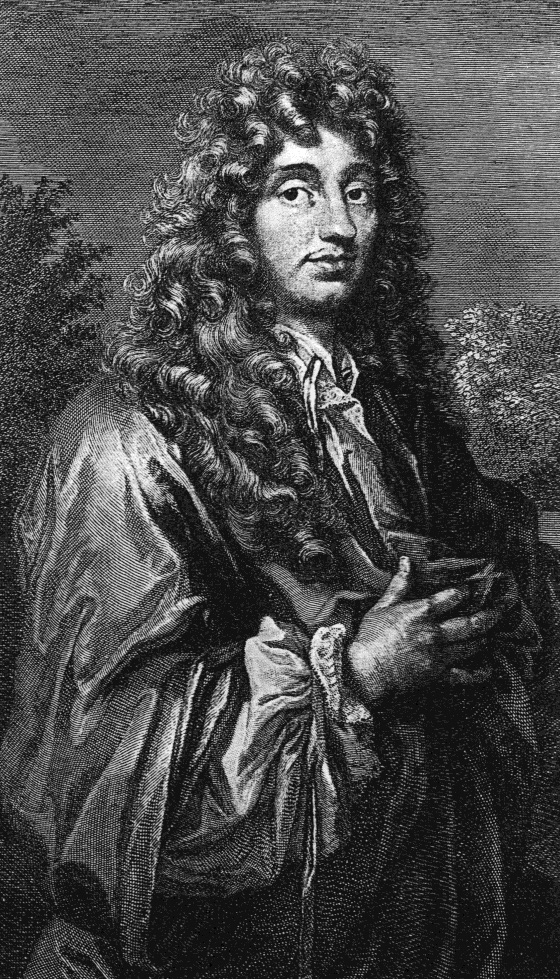
\includegraphics[width=\linewidth]{Christiaan_Huygens.jpg}
  \caption{Christiaan Huygens had sausage fingers}
  \label{fig:marginfig}
\end{marginfigure}
Huygens principle states that every point which a luminous disturbance reaches becomes a source of a spherical wave.  In other words, all points bombarded by waves become point sources for waves.


\section{Interference}
Light wave interference requires the following criteria.
\begin{itemize}
  \item Sources must be coherent, namely maintain a constant phase relative to one another.
  \item Sources must be monochromatic, namely be of a single wavelength.
  \item Superposition must apply
\end{itemize}

\section{Double Slit Experiment}
\begin{marginfigure}[30pt]
  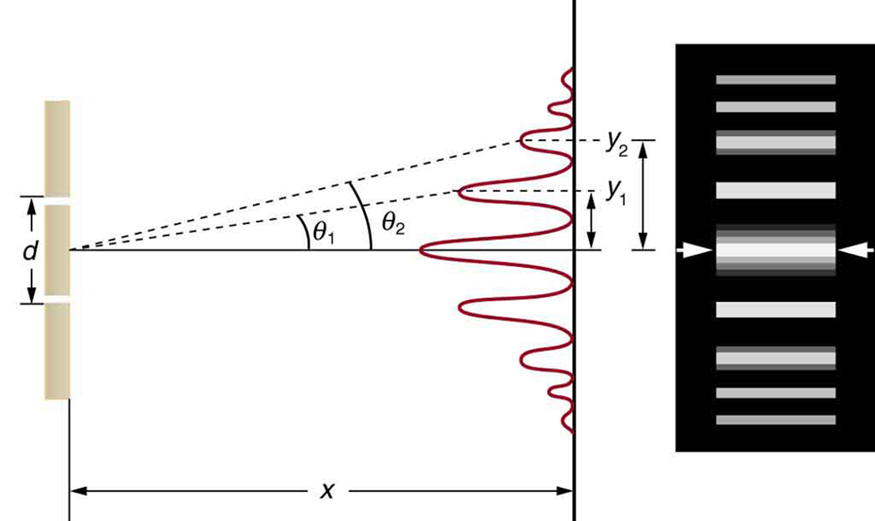
\includegraphics[width=\linewidth]{diffraction.jpg}
  \caption{Two slit diffraction}
  \label{fig:marginfig}
\end{marginfigure}
Conducted by Young 1801.  Consider two slits separated by a distance $d$.  Light interferes on a plane distance $L$ away.  For $L>>d$ we may use parallel ray approximation to determine path difference $\delta$.  
\begin{marginfigure}[10pt]
  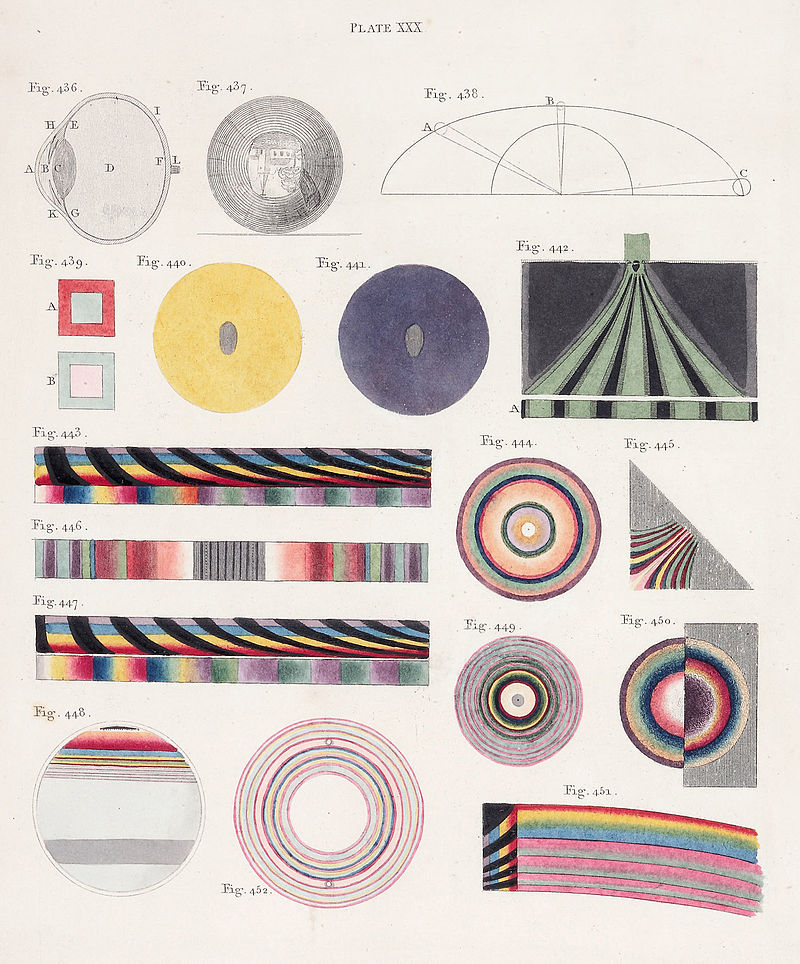
\includegraphics[width=\linewidth]{Young_Plate.jpg}
  \caption{Plate from Thomas Young's 1807 \textit{Lectures on Natural Philosophy and the Mechanical Arts}}
  \label{fig:marginfig}
\end{marginfigure}
$$\delta=r_2-r_1=d\sin\theta$$
Constructive interference associated with bright spots on the plane.
$$d\sin\theta=N\lambda$$
Similar phenomena for a diffraction grating where $d$ is the distance between slits.
 
 \subsection{Intensity}
 Phase difference is related to the path difference and wavelength.
 $$\phi=\frac{2\pi}{\lambda}\delta=\frac{2\pi}{\lambda}d\sin\theta$$
 The total electric field is the sum of the two components of electric field. 
 $$E_T=E_1+E_2=E_0\cos(\omega t)+E_0\cos(\omega t+\phi)=2E_0\cos(\phi/2)\cos(\omega t +\phi/2)$$
 Then relating the average intensity to the average electric field squared removes the time dependence and yields the following. 
 $$I_{avg}=I_0\cos^2\left(\frac{\pi d \sin \theta}{\lambda}\right)$$
 
  \vspace{1cm}
 
 \section{Reflection Phase Change}
 An electromagnetic wave undergoes a phase change of 180 degrees upon reflection at an interface with a medium medium of higher refractive index than the one in which the wave is traveling.  (reflection off a window)
 

 
 \section{Thin Film Interference}
 
 Consider a thin film of refractive index $n$ and thickness $l$.  An electromagnetic wave in air hits the interface, part of the wave is reflected with a 180 degree phase change and part is transmitted into the film.  The transmitted component reflects off the other side of the film and is transmitted bad through the original interface to recombine with the reflected component.
 \begin{marginfigure}[-40pt]
  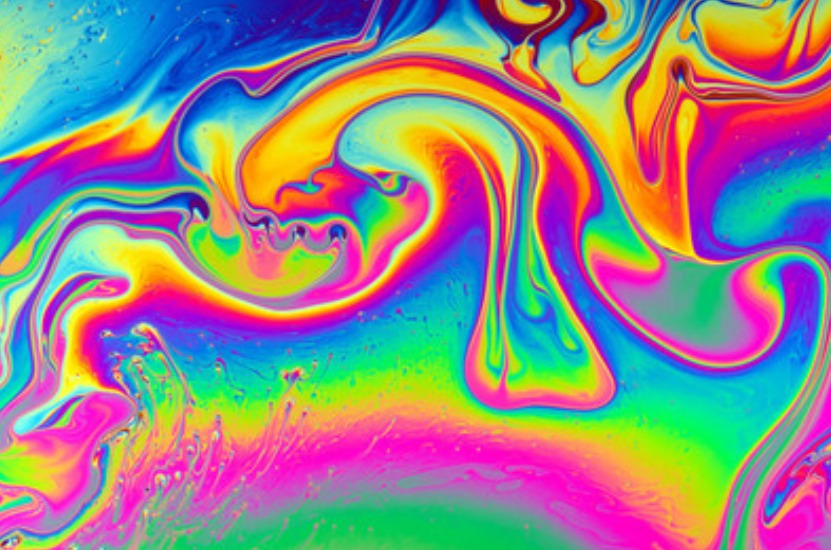
\includegraphics[width=\linewidth]{oil_rainbow.jpg}
  \caption{Thin film of oil}
  \label{fig:marginfig}
\end{marginfigure}

\marginnote[30pt]{
\subsection{Iridescence}
Iridescence caused by thin-film interference is a commonly observed phenomenon in nature, being found in a variety of plants and animals. One of the first known studies of this phenomenon was conducted by Robert Hooke in 1665. In \textit{Micrographia}, Hooke postulated that the iridescence in peacock feathers was caused by thin, alternating layers of plate and air. In 1704, Isaac Newton stated in his book, \textit{Opticks}, that the iridescence in a peacock feather was due to the fact that the transparent layers in the feather were so thin. In 1801, Thomas Young provided the first explanation of constructive and destructive interference.}

 \subsection{Constructive Interference}
 For constructive interference to occur the path difference must be equivalent an integer multiple of wavelengths plus half a wavelength.  This is due to the fact that there is a reflection which takes place.  This is equivalent to a half-phase shift.
 $$2l=\left(N+\frac{1}{2}\right)\frac{\lambda}{n}$$
 Constructive interference is desired for reflective coatings.
  \subsection{Destructive Interference}
  For destructive interference to occur the path difference must be an integer multiple of waves.  The integer multiple of wave will produce destructive interference because there is an additional half-phase shift due to the reflection
 $$2l=N\frac{\lambda}{n}$$
 Destructive interference is desired for anti-glare coatings.
 

\chapter{Relativity}

\textit{Imagination is more important than knowledge. Knowledge is limited. Imagination encircles the world.}\\
\noindent\textbf{-   Albert Einstein}

\vspace{0.5cm}

\begin{marginfigure}%
  \includegraphics[width=\linewidth]{space_time_energy.jpg}
  \caption{Special and general relativity}
  \label{fig:marginfig}
\end{marginfigure}

The theory of relativity usually encompasses two theories by Albert Einstein: special relativity and general relativity.  Concepts introduced by the theories of relativity include spacetime as a unified entity of space and time, relativity of simultaneity, kinematic and gravitational time dilation, and length contraction.

\section{Galilean-Newtonian Relativity}
\begin{marginfigure}[0pt]
  \includegraphics[width=\linewidth]{mboat.jpg}
  \caption{Galilean boat}
  \label{fig:marginfig}
\end{marginfigure}
Galilean invariance, Galilean relativity or Newtonian relativity states Newtonian physics operates the same in all inertial (non-accelerating) frames. Galileo Galilei first described this principle in 1632 in his \textit{Dialogue Concerning the Two Chief World Systems}.  He describes a ship traveling at constant velocity, without rocking, on a smooth sea.  In this ship any observer doing experiments below the deck would not be able to tell whether the ship was moving or stationary.\\
Unfortunately Galilean invariance did not agree with Maxwell's equations describing electromagnetism.  The first problem is that electromagnetic theory describes electromagnetic waves, namely light, moving at a constant speed no matter the velocity of the frame of reference.  In addition all experiments show light moving at a constant speed.  The second problem with electromagnetic theory is that electromagnetic forces seem to be dependent on the velocity of the frame of reference.  Namely, in a frame moving with a charged particle there are no magnetic forces however the same particle observed from a frame in which it is moving could see magnetic forces.  Forces, however, should not be dependent on the velocity of the frame of reference. 

\marginnote[-150pt]{
\subsection{Galilean Transformation}
$x$ transforms to $x'$ in a frame moving in the x-direction at speed $v$.
$$\overrightarrow{v}=v\hat{x}$$
$$x'= x-vt \hspace{2cm} y'=y$$
$$z'= z \hspace{2cm} t'=t$$
$$\overrightarrow{u}'=\overrightarrow{u}-\overrightarrow{v}$$
$$\overrightarrow{E}'=\overrightarrow{E}-\overrightarrow{v}\times\overrightarrow{B}$$
$$\overrightarrow{B}'=\overrightarrow{B}+\frac{1}{c^2}\overrightarrow{v}\times\overrightarrow{E}$$
}


\section{Einstein's Relativity}
Einstein's relativity dictates the laws of mechanics, including electromagnetism, must be the same in all inertial frames and that the speed of light is constant. 

\section{Time Dilation}
\begin{marginfigure}%
  \includegraphics[width=\linewidth]{slow_clock.jpg}
  \caption{Moving clocks run slowly}
  \label{fig:marginfig}
\end{marginfigure}
Consider a light clock which consists of a light source next to a photocell opposite a mirror.  They are a distance $D$ apart.  Light travels at speed $c$ and travels a distance $2D$.  The time it takes is $\Delta \tau$
$$\Delta \tau=\frac{2D}{c}$$
Now consider the light clock moving perpendicular to the length $D$ at a speed $v$.  In this frame the light takes a longer path but still travels at speed $c$.  The time for the light to travel in this frame is $\Delta t'$.
$$\Delta t=\frac{2\sqrt{D^2+(\nicefrac{v \Delta t}{2})^2}}{c}$$
Squaring each side of both equations.
$$(\Delta \tau)^2=\frac{4D^2}{c^2} \hspace{1cm} (\Delta t)^2=\frac{4D^2+v^2(\Delta t)^2}{c^2}$$
\marginnote[-100pt]{$\Delta \tau $ is the proper time interval.  This is defined as the time separating two events that take place at the same point in space. }
Combining these equations and solving for $\Delta t$ yields the following.
$$\Delta t=\frac{\Delta \tau}{\sqrt{1-\frac{v^2}{c^2}}}=\gamma \Delta \tau $$
Note the factor $\nicefrac{1}{\sqrt{1-\nicefrac{v^2}{c^2}}}$ is always greater than one, $\gamma>1$.  Therefore   $\Delta t > \Delta \tau$.  The clock tics more slowly when it is observed moving.
\begin{figure}%
  \includegraphics[width=\linewidth]{time_dilation.jpg}
  \caption{Time dilation}
  \label{fig:marginfig}
\end{figure}


\section{Length Contraction}

\begin{marginfigure}[180pt]
  \includegraphics[width=\linewidth]{LorentzContraction.jpg}
  \caption{Length contraction}
  \label{fig:marginfig}
\end{marginfigure}
Now consider measuring the velocity of an object.  This always requires retrieving information from each frame of reference.  One could view a moving clock and measure the distance it moved between flashes.  The time measurement would be in the moving frame $\Delta t$ while the length measurement would be in the rest frame $L$.  
$$v=\frac{L}{\Delta t}$$
Alternately the velocity could be determined using a still clock with proper time interval $\Delta \tau$ and an object whose length is measured while moving $l$.
$$v=\frac{l}{\Delta \tau}$$
Equating the velocities gives the following.
$$\frac{L}{\Delta t}=\frac{l}{\Delta \tau}$$
Expressing $\Delta \tau$ in terms of $\Delta t$ gives an expression for $L$ in terms of $l$.
$$\frac{L}{	\gamma \Delta \tau}=\frac{l}{\Delta \tau}$$
$$L=\gamma l=\frac{l}{\sqrt{1-\frac{v^2}{c^2}}}$$
This means the moving length $l$ is shorter than the proper length $L$.  This is known as length contraction.  Moving objects appear squished.
\marginnote[-100pt]{$L$ is the proper length.  The proper length or rest length refers to the length of an object in the object's rest frame. }


\section{Lorentz Transformation}
\begin{marginfigure}[50pt]
  \includegraphics[width=\linewidth]{Einstein_Lorentz.jpg}
  \caption{Albert Einstein and Hendrik Lorentz \#biffles4life}
  \label{fig:marginfig}
\end{marginfigure}

The Lorentz transformation is a coordinate transformation between two coordinate frames that move at constant velocity relative to each other.  Here $x$ is transformed to $x'$ by taking measurements in a frame moving at $\overrightarrow{v}=v\hat{x}$.  $$x'= \gamma(x-vt)$$ 
The $y$ and $z$ coordinates are left invariant in this transformation.  
$$ y'=y \hspace{2cm}z'= z$$
Time is transformed in the moving frame as follows.
$$ \hspace{2cm} t'=\gamma \left( t -\frac{v}{c^2}x\right)$$
The velocity of an object in the rest frame is measured as $\overrightarrow{u}$.  The x-component of the velocity is transformed as follows.
$$u_x'=\frac{u_x-v}{1-\frac{u_xv}{c^2}}$$

\section{Relativistic Mechanics}
Special relativity gives new definitions to momentum and kinetic energy.
$$\overrightarrow{p}=m \overrightarrow{v}=\gamma m_0 \overrightarrow{v}$$
\marginnote[-20pt]{An interpretation relativistic momentum uses the concept of relativistic mass.  At high velocity the mass transforms from the rest mass $m_0$ to $m$.
$$m=\gamma m_0$$}
Once relativistic momentum is defined the relativistic force may be derived using Newton's second law.
$$\overrightarrow{F}_{net}=\frac{d\overrightarrow{p}}{dt}$$
Once the relativistic force is defined the relativistic kinetic energy may be derived using work-energy theorem.
$$\Delta KE=W_{net}= \int \overrightarrow{F}_{net}\cdot d\overrightarrow{r}$$
This yields the following expression for relativistic kinetic energy.
$$KE=\gamma m_0c^2-m_0c^2= m c^2-m_0c^2$$
The kinetic energy is the difference between two terms.  The first term $E$ changes with velocity.  The second term, know as the rest energy $E_0$ is independent of velocity.
$$KE=E-E_0$$
The total energy $E$ is defined as the sum of the kinetic energy and the rest energy.
$$E=KE+E_0$$
The total energy and rest energy are written as follows.
$$E=\gamma mc^2$$
\marginnote[0pt]{$$E^2=p^2c^2+(mc^2)^2$$}
$$E_0=m_0c^2$$
This expression for the rest energy describes a relationship between energy and mass.  This is known as mass-energy equivalence.

\section{General Relativity}
\begin{marginfigure}[0pt]
  \includegraphics[width=\linewidth]{EinsteinBoat.jpg}
  \caption{Einstein on a boat!}
  \label{fig:marginfig}
\end{marginfigure}
General relativity describes the effect of gravity on spacetime.  Mass is an inertial quantity.  Newton's second law relates to inertial mass.  
$$F_{net}=m_{i}a$$ 
Gravity is different than the other forces in nature because mass gives rise to its field interaction.
$$F_g=m_gg$$.  
Therefore the strength of the gravitational field $g$ is equal to the acceleration $a$.  The equivalence principle states that a gravitational field is indistinguishable from acceleration.  This gives the theory the ability to analyze the behavior of time, space and light in proximity to mass.\\
The net time dilation in a spherically symmetric gravitational field can is considered. It is written below.
$$\Delta t=\frac{\Delta \tau}{\sqrt{1-\frac{2GM}{rc^2}}}=\frac{\Delta \tau}{\sqrt{1-\frac{v_e^2}{c^2}}}$$
\begin{marginfigure}[-60pt]
  \includegraphics[width=\linewidth]{Einstein14.jpg}
  \caption{Albert Einstein at 14}
  \label{fig:marginfig}
\end{marginfigure}
The proper time is outside the gravitational field, out at $r=\infty$.  Note that this is simply special relativity applied when the object is moving at the escape velocity from the field.
Other effects include bending of light and curvature of space.

\chapter{Quantum Mechanics}

\textit{The solution of the difficulty is that the two mental pictures which experiment lead us to form - the one of the particles, the other of the waves - are both incomplete and have only the validity of analogies which are accurate only in limiting cases.}\\
\noindent\textbf{-   Werner Heisenberg}

\vspace{0.5cm}

\begin{marginfigure}[-130pt]
  \includegraphics[width=\linewidth]{snowden.jpg}
  \caption{Snowden says NSA is building a quantum computer}
  \label{fig:marginfig}
\end{marginfigure}

A quantum (plural: quanta) is the minimum amount of any physical quantity involved in an interaction.  For example, angular momentum $J$ is quantized into units $\hbar$.
$$J_n=n\hbar$$
Quantum mechanics describes systems with probability distributions in space and time.  The probabilities describe discrete particle events.  The structure of those distributions however have wavelike features.  This is known as wave particle duality.
Quantum mechanics gradually arose from Max Planck's solution in 1900 to the black-body radiation problem and Albert Einstein's 1905 paper which offered a quantum-based theory to explain the photoelectric effect (reported 1887). 

\section{Blackbody Radiation}
\subsection{Rayleigh-Jeans Law (Classical)}
\marginnote[-260pt]{In 1900, the British physicist Lord Rayleigh derived the $\lambda^{-4}$ dependence of the Rayleigh-Jeans law based on classical physical arguments and empirical facts.  The proportionality constant was added by Rayleigh and Sir James Jeans in 1905. The Rayleigh-Jeans law revealed an important error in physics theory of the time as it predicted an energy output that diverges towards infinity as wavelength approaches zero and energy output at short wavelengths disagreed with this prediction.
This was known as the ultraviolet catastrophe.  The term "ultraviolet catastrophe" was first used in 1911 by Paul Ehrenfest, but the concept originated with the 1900 derivation of the Rayleigh-Jeans law. The phrase refers to the fact that the Rayleigh-Jeans law accurately predicts experimental results at radiative frequencies below 105 GHz, but begins to diverge with empirical observations as these frequencies reach the ultraviolet region of the electromagnetic spectrum}
\begin{marginfigure}[10pt]
  \includegraphics[width=\linewidth]{raleigh.jpg}
  \caption{Ultraviolet catastrophe}
  \label{fig:marginfig}
\end{marginfigure}
The Rayleigh-Jeans law attempts to describe the spectral radiance of electromagnetic radiation at all wavelengths from a black body at a given temperature through classical arguments.
$$I(\lambda,T)=\frac{2\pi c k_B T}{\lambda^4}$$
In 1838, Michael Faraday discovered cathode rays. By 1859 the black-body radiation problem had been identified by Gustav Kirchhoff. 
\subsection{Planck Spectrum (Modern)}
Ludwig Boltzmann suggested that the energy states of a physical system can be discrete in 1877 and by 1900 the quantum hypothesis had ben made by Max Planck.  The hypothesis states that energy is radiated and absorbed in discrete "quanta" (or energy elements).  Statistically this models the intensity $I$ as a particular function of wavelength and temperature.  This distribution is known as the Planck spectrum.
$$I(\lambda,T)=\frac{2\pi h c^2 }{\lambda^5\left(e^{\frac{hc}{\lambda k_B T}}-1\right)}$$
The Planck spectrum precisely matched the observed patterns of black-body radiation.  Specifically it matched Wien's displacement law.
\marginnote[-180pt]{
\begin{itemize}
  \item Molecules have discrete energy states $E_n$
  $$E_n=nhf $$
   \item Energy is released in discrete packets of electromagnetic radiation called "photons"
   $$E_{photon}=hf $$
\end{itemize}}
\begin{marginfigure}[-80pt]
  \includegraphics[width=\linewidth]{planck_spectrum.jpg}
  \caption{Planck spectrum}
  \label{fig:marginfig}
\end{marginfigure}

Wien's displacement law states that the black body radiation curve for different temperatures peaks at a wavelength inversely proportional to the temperature. 
$$\lambda_{peak}=\frac{2900\ \mu \text{m}\cdot\text{K}}{T}$$
The shift of that peak is a direct consequence of the Planck radiation law which describes the spectral brightness of black body radiation as a function of wavelength at any given temperature. However it had been discovered by Wilhelm Wien several years before Max Planck developed that more general equation, and describes the entire shift of the spectrum of black body radiation toward shorter wavelengths as temperature increases.


\begin{marginfigure}[-50pt]
  \includegraphics[width=\linewidth]{planck.jpg}
  \caption{Young Max Planck }
  \label{fig:marginfig}
\end{marginfigure}

\begin{marginfigure}[0pt]
  \includegraphics[width=\linewidth]{PE_effect.jpg}
  \caption{Photoelectric tube }
  \label{fig:marginfig}
\end{marginfigure}
\section{Photoelectric Effect}
The photoelectric effect is the observation that many metals emit electrons when light shines upon them. Electrons emitted in this manner can be called photoelectrons.  

According to classical electromagnetic theory, this effect can be attributed to the transfer of energy from the light to an electron in the metal. From this perspective, an alteration in either the intensity or wavelength of light would induce changes in the rate of emission of electrons from the metal. Furthermore, according to this theory, a sufficiently dim light would be expected to show a time lag between the initial shining of its light and the subsequent emission of an electron. However, the experimental results did not correlate with either of the two predictions made by classical theory.

Instead, electrons are only dislodged by the impingement of photons when those photons reach or exceed a threshold frequency. Below that threshold, no electrons are emitted from the metal regardless of the light intensity or the length of time of exposure to the light. To make sense of the fact that light can eject electrons even if its intensity is low, Albert Einstein proposed that a beam of light is not a wave propagating through space, but rather a collection of discrete wave packets (photons), each with energy hf. This shed light on Max Planck's previous discovery of the Planck relation (E = hf) linking energy (E) and frequency (f) as arising from quantization of energy. The factor h is known as the Planck constant.

In 1887, Heinrich Hertz discovered that electrodes illuminated with ultraviolet light create electric sparks more easily. In 1905 Albert Einstein published a paper that explained experimental data from the photoelectric effect as the result of light energy being carried in discrete quantized packets. This discovery led to the quantum revolution.
The work function $W$ is the work required to free an electron from the metal.  
\begin{marginfigure}[-80pt]
  \includegraphics[width=\linewidth]{PE_graph.jpg}
  \caption{Photoelectric effect graph}
  \label{fig:marginfig}
\end{marginfigure}
$$KE_{max}=hf-W$$
$$KE_{max}=eV_{stop}$$

Electrons will not be emitted if incident light is below a certain cutoff frequency even if intensity of light is increased.  

\section{Compton Effect}
Compton scattering, discovered by Arthur Holly Compton, is the inelastic scattering of a photon by a charged particle, usually an electron.\marginnote[100pt]{ Compton scattering results in a decrease in energy (increase in wavelength) of the photon.  This is called the Compton effect. Part of the energy of the photon is transferred to the recoiling electron.  The scattering supports particle nature of light.}
$$\lambda'-\lambda_0=\frac{h}{mc}\left(1-\cos \theta\right)$$

\begin{figure}
  \includegraphics[width=\linewidth]{compton.jpg}
  \caption{Compton scattering}
  \label{fig:fig}
\end{figure}

\section{De Broglie Relation}\marginnote[0pt]{\subsection{Planck-Einstein Relation}
$$E=\frac{h}{T}=hf=\hbar \omega$$}
All matter can exhibit wave-like behavior. For example, a beam of electrons can be diffracted just like a beam of light or a water wave. Matter waves are a central part of the theory of quantum mechanics, being an example of wave-particle duality. The concept that matter behaves like a wave is also referred to as the de Broglie hypothesis due to having been proposed by Louis de Broglie in 1924.  Matter waves are often referred to as de Broglie waves.\\
The De Broglie wavelength is the wavelength, $\lambda$, associated with a massive particle and is related to its momentum, $p$, through the Planck constant, $h$.
$$p=\frac{h}{\lambda}=\hbar k$$
\begin{marginfigure}[0pt]
  \includegraphics[width=\linewidth]{debroglie.jpg}
  \caption{Louis De Broglie}
  \label{fig:marginfig}
\end{marginfigure}
De Broglie, in his 1924 PhD thesis, proposed that just as light has both wave-like and particle-like properties, electrons also have wave-like properties.




\section{Wave functions}
\marginnote{
\subsection{Probability distributions}
For standard probability distributions average values are calculated as follows.
$$\Braket{x}=\int^\infty_{-\infty}\rho(x)x \ dx$$
$$\Braket{x^2}=\int^\infty_{-\infty}\rho(x)x^2 \ dx$$
$$\int^\infty_{-\infty}\rho(x) \ dx=1$$
} 



In quantum mechanics a wave function is a mathematical object that represents a particular pure quantum state of a specific isolated system of one or more particles. It is a central entity in quantum mechanics and provides probability distribution of states. 
$$\psi(x,t)=Ae^{-i\left(kx-\omega t\right)}=A\left( \cos \left( k x-\omega t \right)+i\sin \left( k x-\omega t \right) \right)$$
 These distributions can be used to find average values of observable quantities as follows.
$$\Braket{x}=\int^\infty_{-\infty}\psi^*(x)x\ \psi(x) \ dx$$
The wave functions provide an inner product space for a set of observable operators.  The DeBroglie relation is represented through the following momentum operator.
$$\Braket{p}=\int^\infty_{-\infty}\psi^*(x)\left(i \hbar \frac{d}{dx}\right)\ \psi(x) \ dx$$
\marginnote[-40pt]{$$i \hbar \frac{d}{dx}e^{-i\left(kx-\omega t\right)}=-i^2 \hbar k e^{-i\left(kx-\omega t\right)}$$
$$i \hbar \frac{d}{dx}e^{-i\left(kx-\omega t\right)}=p e^{-i\left(kx-\omega t\right)}$$}
The Planck-Einstein relation is represented through the following Hamiltonian (energy operator).
$$\Braket{H}=\int^\infty_{-\infty}\psi^*(x,t)\left(i \hbar \frac{d}{dt}\right)\ \psi(x,t) \ dx$$
\marginnote[-40pt]{$$i \hbar \frac{d}{dt}e^{-i\left(kx-\omega t\right)}=-i^2 \hbar \omega e^{-i\left(kx-\omega t\right)}$$
$$i \hbar \frac{d}{dt}e^{-i\left(kx-\omega t\right)}=E e^{-i\left(kx-\omega t\right)}$$}
The inner product of the wavefunction should be normalized.
$$\int^\infty_{-\infty}\psi^*(x) \psi(x) \ dx=1$$


\section{Schrodinger Equation}
\begin{marginfigure}
  \includegraphics[width=\linewidth]{Schrodinger.jpg}
  \caption{Erwin Schrodinger}
  \label{fig:fig}
\end{marginfigure}
\begin{marginfigure}[30pt]
  \includegraphics[width=\linewidth]{schrodingers_cat.jpg}
  \caption{Schrodinger's cat}
  \label{fig:fig}
\end{marginfigure}

The Schr�dinger equation is the fundamental equation of physics for describing quantum mechanical behavior. It is also often called the Schr�dinger wave equation, and is a partial differential equation that describes how the wavefunction of a physical system evolves over time. Viewing quantum mechanical systems as solutions to the Schr�dinger equation is sometimes known as the Schr�dinger picture, as distinguished from the matrix mechanical viewpoint, sometimes known as the Heisenberg picture.
$$\mathcal{H}\psi(x,t)=\frac{p^2}{2m}\psi(x,t)+V(x)\psi(x)=E\psi(x,t)$$
$$\frac{-\hbar^2}{2m}\frac{d^2}{dx^2}\psi(x,t)+V(x)\psi(x)=E\psi(x,t)$$
$$\frac{d^2}{dx^2}\psi(x,t)=-\frac{2m}{\hbar^2}\left[E-V(x)\right]\psi(x,t)$$

\section{Uncertainty Relations}
 The uncertainty principle, also known as Heisenberg's uncertainty principle, is any of a variety of mathematical inequalities asserting a fundamental limit to the precision with which certain pairs of physical properties of a particle, known as complementary variables, such as position $x$ and momentum p, can be known simultaneously.  Introduced first in 1927, by the German physicist Werner Heisenberg, it states that the more precisely the position of some particle is determined, the less precisely its momentum can be known, and vice versa
$$(\Delta x)^2=\Braket{x^2}-\Braket{x}^2$$
The uncertainty of a quantity is calculated from the difference between the mean square and the square mean.  The relationship between the uncertainty in position and momentum is as follows.
\marginnote[-80pt]{$$\sigma_x=\Delta x$$
$$\sigma_p=\Delta p$$}
\marginnote[-40pt]{
According to the Copenhagen interpretation, physical systems generally do not have definite properties prior to being measured, and quantum mechanics can only predict the probabilities that measurements will produce certain results. The act of measurement affects the system, causing the set of probabilities to reduce to only one of the possible values immediately after the measurement. This feature is known as wavefunction collapse.\\
Schr�dinger's cat is a thought experiment, sometimes described as a paradox, devised by Austrian physicist Erwin Schr�dinger in 1935. It illustrates what he saw as the problem of the Copenhagen interpretation of quantum mechanics applied to everyday objects. }
$$\Delta x\ \Delta p\geq  \frac{\hbar}{2}$$
The relationship between the uncertainty in energy and time is as follows.
$$\Delta E\ \Delta t\geq \frac{\hbar}{2}$$
As a mathematical system for making statements about the world, quantum mechanics has limits of specificity built in.  These uncertainties are not shortcomings of measurement.  They are hard coded into quantum theory itself.

\section{Particle in a Box}
\begin{marginfigure}[0pt]
  \includegraphics[width=\linewidth]{particle_box.jpg}
  \caption{Particle in a box wavefunctions}
  \label{fig:fig}
\end{marginfigure}

the particle in a box model (also known as the infinite potential well or the infinite square well) describes a particle free to move in a small space surrounded by impenetrable barriers. The model is mainly used as a hypothetical example to illustrate the differences between classical and quantum systems. In classical systems, for example a ball trapped inside a large box, the particle can move at any speed within the box and it is no more likely to be found at one position than another. However, when the well becomes very narrow (on the scale of a few nanometers), quantum effects become important. The particle may only occupy certain positive energy levels. Likewise, it can never have zero energy, meaning that the particle can never "sit still". Additionally, it is more likely to be found at certain positions than at others, depending on its energy level. The particle may never be detected at certain positions, known as spatial nodes.
\marginnote[20pt]{$$\sigma_x^2=\frac{L^2}{12}\left(1-\frac{6}{n^2\pi^2}\right)$$
$$\sigma_p^2=\left(\frac{\hbar n\pi}{L}\right)^2$$
$$\sigma_x \sigma_p = \frac{\hbar}{2} \sqrt{\frac{n^2\pi^2}{3}-2}$$}
$$ \psi(x)=A\sin\left(\frac{n\pi x}{L}\right)$$
$$E_n=\frac{h^2n^2}{8mL^2}$$

\section{Hydrogen Atom and the Bohr Model}
\marginnote{
The principal quantum number (symbolized $n$) is one of four quantum numbers which are assigned to each electron in an atom to describe that electron's state. As a discrete variable, the principal quantum number is always an integer. As $n$ increases, the number of electronic shells increases and the electron spends more time farther from the nucleus. As $n$ increases, the electron is also at a higher potential energy and is therefore less tightly bound to the nucleus.

The principal quantum number was first created for use in the semiclassical Bohr model of the atom, distinguishing between different energy levels. With the development of modern quantum mechanics, the simple Bohr model was replaced with a more complex theory of atomic orbitals. However, modern theory still requires the principal quantum number.
 Apart from the principal quantum number $n$, the other quantum numbers for bound electrons are the azimuthal quantum number $l$, the magnetic quantum number $m$, and the spin quantum number $s$.}

 The 1913 Niels Bohr paper \textit{On the Constitution of Atoms and Molecules} depicts the atom as a small, positively charged nucleus surrounded by electrons that travel in circular orbits around the nucleus.  It is the solar system, but small and attraction provided by electrostatic forces rather than gravity.
 \subsection{Ryberg Formula}
The model's key success lay in explaining the Rydberg formula for the spectral emission lines in of atomic hydrogen.
$$\frac{1}{\lambda} = R\left(\frac{1}{n_1^2}-\frac{1}{n_2^2}\right) $$
The Ryberg constant  $R$ fits the spectral lines of hydrogen with the following value.
$$R=\frac{1.097 \times 10^{7}}{\text{m}}$$
While the Rydberg formula had been known experimentally, it did not gain a theoretical underpinning until the Bohr model was introduced.


\begin{figure*}
  \includegraphics[width=\linewidth]{HydrogenSpectrum.jpg}
  \caption{Hydrogen spectrum}
  \label{fig:fig}
\end{figure*}

\subsection{Quantization of Angular Momentum}
In order to derive the energy levels of the Bohr model begin with quantization of angular momentum.
$$L=n\hbar=mvr$$
This is the quantum fairy dust sprinkled on circular orbits of the electron in a Coulomb field.
\marginnote[-70pt]{\subsection{Coulomb Force}
In this case the Coulomb force provides the centripetal force.
$$F_e=F_c$$
For an electron orbiting a proton the following applies.
$$ \frac{k_ee^2}{r^2}=\frac{m_ev^2}{r}$$
This is useful to parameterize the kinetic energy as a function of radius. 
\subsection{Energy}
Consider the total energy of the hydrogen atom.
$$E=KE+PE$$
$$E=\frac{m_ev^2}{2}-\frac{k_ee^2}{r}$$
Substituting yields a function for the total energy as a function of $r$ or of $v$.
$$E=-\frac{k_ee^2}{2r}=-\frac{m_ev^2}{2}$$
This is used to derive an expression for the radius of orbit $r$ as a function of $v$.
}
\subsection{Orbital Radii}
Applying the quantization of angular momentum yields the following.
$$r= \frac{k_ee^2}{mv^2} \hspace{2cm} v=\frac{n\hbar}{mr}$$
This process identifies the quantized orbital radii of hydrogen.  Remember $n$ is tracking the angular momentum of the hydrogen atom.
$$r_n=\frac{n^2\hbar^2}{m_ek_ee^2}=n^2a_0$$
From the quantized radii the energy levels may be expressed.
$$E_n=-\frac{k_ee^2}{2a_0n^2}=\frac{E_1}{n^2}$$
The wavelength of photon emitted from an electron transition from $m$ to $n$ is written.
$$E_n-E_m=\frac{hc}{\lambda}$$
The Ryberg constant may be identified.
$$R=\frac{E_1}{hc}$$
\marginnote[-80pt]{ \subsection{Quantum Stability}
Experiments by Rutherford in 1909 showed the structure of the atom be a dense, positive nucleus with a light, negative charge orbiting around it. This immediately caused problems on how such a system could be stable. Classical electromagnetism had shown that any accelerating charge radiates energy described through the Larmor formula. If the electron is assumed to orbit in a perfect circle and radiates energy continuously, the electron would spiral into the nucleus.
$$P = {2 \over 3} \frac{q^2 a^2}{  4 \pi \varepsilon_0 c^3}= \frac{q^2 a^2}{6 \pi \varepsilon_0 c^3} \mbox{ (SI units)}$$ 
$$t_\text{fall} \approx \frac{ a_0^3}{4 r_0^2 c} \approx 1.6 \cdot 10^{-11} \text{s}$$}
\section{Schrodinger's Hydrogen}
$$\left(- \frac{\hbar^2}{2 \mu} \nabla^2  - \frac{ Z e^2}{4 \pi \epsilon_0 r} \right) \psi(r,\theta, \phi) = E \psi(r, \theta, \phi)$$
Above is the Schrodinger equation for 3-dimensions.  Expanding in sperical coordinates leaves the following.
\begin{fullwidth}
$$-\frac{\hbar^2}{2 \mu} \left[ \frac{1}{r^2} \frac{\partial }{\partial r} \left( r^2 \frac{ \partial \psi}{\partial r}\right) + \frac{1}{r^2 \sin \theta} \frac{\partial }{\partial \theta} \left( \sin \theta \frac{\partial \psi}{\partial \theta}\right) + \frac{1}{r^2 \sin^2 \theta} \frac{\partial^2 \psi}{\partial \phi^2} \right] - \frac{Z e^2}{ 4 \pi \epsilon_0 r} \psi= E \psi$$
\end{fullwidth}
The solution of the Schr�dinger equation wave equation for the hydrogen atom is written as follows.$$ \psi_{n\ell m}(r,\vartheta,\varphi) = \sqrt {{\left (  \frac{2}{n a_0} \right )}^3 \frac{(n-\ell-1)!}{2n[(n+\ell)!]}} e^{- \rho / 2} \rho^{\ell} L_{n-\ell-1}^{2\ell+1}(\rho) Y_{\ell}^{m}(\vartheta, \varphi ) $$
$$ \rho = {2r \over {na_0}} $$
\begin{marginfigure}
  \includegraphics[width=\linewidth]{Hydrogen_Density_Plots.jpg}
  \caption{Hydrogen wave function}
  \label{fig:fig}
\end{marginfigure}
\begin{marginfigure}
  \includegraphics[width=\linewidth]{Lstates.jpg}
  \caption{Quantum numbers $\ell$ and $m$}
  \label{fig:fig}
\end{marginfigure}

$ L_{n-\ell-1}^{2\ell+1}(\rho) $ is the generalized Laguerre polynomial of degree $n-\ell -1$.  Here is a closed form formula.
$$ L_n^{\alpha} (x) = \sum_{i=0}^n (-1)^i {n+\alpha \choose n-i} \frac{x^i}{i!} $$
$Y_{\ell}^{m}(\vartheta, \varphi )$ is the is a spherical harmonic function of degree $\ell$ and order $m$.  Here is a closed form formula.
$$  Y_\ell^m( \theta , \varphi ) = \sqrt{{(2\ell+1)\over 4\pi}{(\ell-m)!\over (\ell+m)!}}  \, P_\ell^m ( \cos{\theta} ) \, e^{i m \varphi } $$
Here $ P_\ell^{m}(x)$ is the associated Legendre polynomial of degree $\ell$ and order $m$.  Here is the Rodriguez formula.
$$ P_\ell^{m}(x) = \frac{(-1)^m}{2^\ell \ell!} (1-x^2)^{m/2}\  \frac{d^{\ell+m}}{dx^{\ell+m}}(x^2-1)^\ell$$


The energy eigenstates may be classified by two angular momentum quantum numbers, $\ell$ and m (both are integers). The angular momentum quantum number $\ell = 0, 1, 2, ...$ determines the magnitude of the angular momentum. The magnetic quantum number $m = -\ell, ..., +\ell$ determines the projection of the angular momentum on the (arbitrarily chosen) z-axis.

The Schrodinger hydrogen is a probability distribution. The ground state is spherically symmetric, in fact all $\ell=0$ states are symmetric.  The average radial position of these probability distribution functions corresponds to the quantized radii of the Bohr atom.
\begin{marginfigure}
  \includegraphics[width=\linewidth]{orbs.jpg}
  \caption{Spherical harmonics}
  \label{fig:fig}
\end{marginfigure}
$$\braket{r}_{n}=n^2a_0$$
Note the $\ell=0$ states correspond to zero angular momentum.  Compare this to the Bohr model ground state.
\section{Harmonic Oscillator}
The quantum harmonic oscillator is the quantum-mechanical analog of the classical harmonic oscillator. Because an arbitrary potential can usually be approximated as a harmonic potential at the vicinity of a stable equilibrium point, it is one of the most important model systems in quantum mechanics. Furthermore, it is one of the few quantum-mechanical systems for which an exact, analytical solution is known.
\marginnote[-80pt]{
$$V(x)=\frac{kx^2}{2}=\frac{m\omega^2x^2}{2}$$
$$E=\frac{m\omega^2A^2}{2}$$
\subsection{Ground State Wavefunction}
$$\psi_0(x)=Be^{-Cx^2}$$
$$C=\frac{m\omega}{2\hbar} \hspace{2cm} E_0=\frac{\hbar \omega}{2}$$

}
$$\frac{d^2}{dx^2}\psi(x)=-\frac{2m}{\hbar^2}\left[E-\frac{m\omega^2x^2}{2}\right]\psi(x)=-\left[\frac{2mE}{\hbar^2}-\left(\frac{m\omega}{\hbar}\right)^2x^2\right]\psi(x)$$

\subsection{Quantized Energy States}
$$E_{n+1}-E_n=\hbar \omega$$
From the ground state it is possible to ladder up the states.  This is the general solution of the wavefunction.
\begin{marginfigure}
  \includegraphics[width=\linewidth]{harmosc.jpg}
  \caption{Quantized harmonic oscillator}
  \label{fig:fig}
\end{marginfigure}
\begin{marginfigure}
  \includegraphics[width=\linewidth]{howave.jpg}
  \caption{Harmonic oscillator wavefunctions}
  \label{fig:fig}
\end{marginfigure}
\begin{marginfigure}
  \includegraphics[width=\linewidth]{harmo.jpg}
  \caption{Harmonic approximation}
  \label{fig:fig}
\end{marginfigure}
$$  \psi_n(x) = \frac{1}{\sqrt{2^n\,n!}} \cdot \left(\frac{m\omega}{\pi \hbar}\right)^{1/4} \cdot e^{
- \frac{m\omega x^2}{2 \hbar}} \cdot H_n\left(\sqrt{\frac{m\omega}{\hbar}} x \right), \qquad n = 0,1,2,\ldots$$
Where $H_n$ are Hermite polynomials.  The Rodriquez formula is written below.
$$H_n(z)=(-1)^n~ e^{z^2}\frac{d^n}{dz^n}\left(e^{-z^2}\right)$$
The quantized energy states are written as follows.
$$ E_n = \hbar \omega \left(n + {1\over 2}\right) = (2 n + 1) {\hbar \over 2} \omega$$
This energy spectrum is noteworthy for three reasons. First, the energies are quantized, meaning that only discrete energy values.  Second, these discrete energy levels are equally spaced, unlike in the Bohr model of the atom, or the particle in a box. Third, the lowest achievable energy (the energy of the n = 0 state, called the ground state) is not equal to the minimum of the potential well, but $\nicefrac{\hbar \omega}{2}$ above it; this is called zero-point energy. Because of the zero-point energy, the position and momentum of the oscillator in the ground state are not fixed (as they would be in a classical oscillator), but have a small range of variance, in accordance with the Heisenberg uncertainty principle. This zero-point energy further has important implications in quantum field theory and quantum gravity.

\section{Spin}

\begin{marginfigure}[20pt]
  \includegraphics[width=\linewidth]{stern_ger.jpg}
  \caption{Stern-Gerlach experiment}
  \label{fig:fig}
\end{marginfigure}
Spin is an intrinsic form of angular momentum carried by elementary particles, composite particles (hadrons), and atomic nuclei.

Spin is one of two types of angular momentum in quantum mechanics, the other being orbital angular momentum. The orbital angular momentum operator is the quantum-mechanical counterpart to the classical angular momentum of orbital revolution: it arises when a particle executes a rotating or twisting trajectory (such as when an electron orbits a nucleus). The existence of spin angular momentum is inferred from experiments, such as the Stern-Gerlach experiment, in which particles are observed to possess angular momentum that cannot be accounted for by orbital angular momentum alone.

\marginnote{In the original Stern-Gerlach experiment, silver atoms were sent through a non-uniform magnetic field, which deflected them before they struck a detector screen. Other kinds of particles can be used. If the particles have a magnetic moment related to their spin angular momentum, the magnetic field gradient deflects them from a straight path. The screen reveals discrete points of accumulation rather than a continuous distribution, owing to the quantum nature of spin. Historically, this experiment was decisive in convincing physicists of the reality of angular momentum quantization in all atomic-scale systems.}

In some ways, spin is like a vector quantity; it has a definite magnitude, and it has a "direction" (but quantization makes this "direction" different from the direction of an ordinary vector). All elementary particles of a given kind have the same magnitude of spin angular momentum, which is indicated by assigning the particle a spin quantum number.

Spin was first discovered in the context of the emission spectrum of alkali metals. In 1924 Wolfgang Pauli introduced what he called a "two-valued quantum degree of freedom" associated with the electron in the outermost shell. This allowed him to formulate the Pauli exclusion principle, stating that no two electrons can share the same quantum state at the same time.

\begin{marginfigure}[20pt]
  \includegraphics[width=\linewidth]{spin_e.jpg}
  \caption{Spin is intrinsic angular momentum}
  \label{fig:fig}
\end{marginfigure}
\section{Dirac Equation}
In particle physics, the Dirac equation is a relativistic wave equation derived by British physicist Paul Dirac in 1928. In its free form, or including electromagnetic interactions, it describes all spin-$\nicefrac{1}{2}$ massive particles such as electrons and quarks, for which parity is a symmetry, and is consistent with both the principles of quantum mechanics and the theory of special relativity, and was the first theory to account fully for special relativity in the context of quantum mechanics. It accounted for the fine details of the hydrogen spectrum in a completely rigorous way.

The equation also implied the existence of a new form of matter, antimatter, previously unsuspected and unobserved and which was experimentally confirmed several years later. It also provided a theoretical justification for the introduction of several-component wave functions in Pauli's phenomenological theory of spin; the wave functions in the Dirac theory are vectors of four complex numbers (known as bispinors), two of which resemble the Pauli wavefunction in the non-relativistic limit, in contrast to the Schr�dinger equation which described wave functions of only one complex value. Moreover, in the limit of zero mass, the Dirac equation reduces to the Weyl equation.
\begin{marginfigure}[0pt]
  \includegraphics[width=\linewidth]{dirac_sea.jpg}
  \caption{Vacuum fluctuations}
  \label{fig:fig}
\end{marginfigure}
Although Dirac did not at first fully appreciate the importance of his results, the entailed explanation of spin as a consequence of the union of quantum mechanics and relativity - and the eventual discovery of the positron - represents one of the great triumphs of theoretical physics. This accomplishment has been described as fully on a par with the works of Newton, Maxwell, and Einstein before him. In the context of quantum field theory, the Dirac equation is reinterpreted to describe quantum fields corresponding to spin-$\nicefrac{1}{2}$ particles.
$$\frac{E^2}{c^2} - p^2 = m^2c^2$$
Starting from the relativistic relation between energy and momentum.
$$-\frac{\hbar^2}{2m}\nabla^2\phi = i\hbar\frac{\partial}{\partial t}\phi.$$
The Schrodinger equation transforms to the Dirac equation.
$$\left(-\frac{1}{c^2}\frac{\partial^2}{\partial t^2} + \nabla^2\right)\phi = \frac{m^2c^2}{\hbar^2}\phi$$
\subsection{Negative Energies}
\begin{marginfigure}[80pt]
  \includegraphics[width=\linewidth]{dirac.jpg}
  \caption{Paul Dirac at CERN}
  \label{fig:fig}
\end{marginfigure}
The negative E solutions to the equation are problematic, for it was assumed that the particle has a positive energy. Mathematically speaking, however, there seems to be no reason for us to reject the negative-energy solutions. Since they exist, we cannot simply ignore them, for once we include the interaction between the electron and the electromagnetic field, any electron placed in a positive-energy eigenstate would decay into negative-energy eigenstates of successively lower energy. Real electrons obviously do not behave in this way, or they would disappear by emitting energy in the form of photons.

To cope with this problem, Dirac introduced the hypothesis, known as hole theory, that the vacuum is the many-body quantum state in which all the negative-energy electron eigenstates are occupied. This description of the vacuum as a "sea" of electrons is called the Dirac sea. Since the Pauli exclusion principle forbids electrons from occupying the same state, any additional electron would be forced to occupy a positive-energy eigenstate, and positive-energy electrons would be forbidden from decaying into negative-energy eigenstates.




\chapter{Nuclear Physics}

\textit{Now I am become Death, the destroyer of worlds.}\\
\noindent\textbf{-    Bhagavad Gita}

\vspace{0.5cm}

\begin{marginfigure}[-10pt]
  \includegraphics[width=\linewidth]{Nuclear_Family.jpg}
  \caption{Nuclear Family (DC Comics)}
  \label{fig:fig}
\end{marginfigure}

\vspace{0.5cm}

Nuclear physics starts with the discovery of radioactivity by Henri Becquerel in 1896, while investigating phosphorescence in uranium salts. The discovery of the electron by J. J. Thomson a year later was an indication that the atom had internal structure. 

At the beginning of the 20th century the accepted model of the atom was J. J. Thomson's "plum pudding" model in which the atom was a positively charged ball with smaller negatively charged electrons embedded inside it.  By 1900 physicists had also discovered three types of radiation emanating from atoms, which they named $\alpha$, $\beta$, and $\gamma$ radiation.  

By 1905, Albert Einstein formulated the idea of mass-energy equivalence. While the work on radioactivity by Becquerel and Marie Curie predates this, an explanation of the source of the energy of radioactivity would have to wait for the discovery that the nucleus itself was composed of smaller constituents, the nucleons.  In 1911 Rutherford scattering helped clarify the model of the atom as having a dense positively charged nucleus.
\marginnote[-150pt]{Satyendra Nath Bose was a Bengali physicist specializing in mathematical physics. He is best known for his work on quantum mechanics in the early 1920s, providing the foundation for Bose-Einstein statistics and the theory of the Bose-Einstein condensate.\\
Bose said Maxwell-Boltzmann distribution would not be true for microscopic particles, where fluctuations due to Heisenberg's uncertainty principle are significant. He theorized probability states in phase space having volumes $h^3$, disregarding the distinct position and momentum of particles.}
\vspace{0.5cm}

\section{Particles}

\begin{marginfigure}[0pt]
  \includegraphics[width=\linewidth]{bose.jpg}
  \caption{Satyendra Nath Bose}
  \label{fig:fig}
\end{marginfigure}

\begin{description}  
\item [Fermions]  Fermions are odd integer half spin particles.  They may be elementary particles or composite particles.  Fermions obey the Pauli exclusion principle, namely no two fermions can occupy the same quantum state.
\item [Bosons] Bosons are integer spin particles.  They may be elementary gauge bosons or composite particles.  Bosons obey Bose-Einstein statistics. Two bosons can occupy the same quantum state.  Cool bosons and they all condense into the ground state.
\item [Quarks]  Quarks are elementary particles and fundamental constituents of matter.  They have spin $\frac{1}{2}$ and are thus fermions.  Their charges are $\frac{2}{3}e$ or $-\frac{1}{3}e$.  There are six types of quarks, known as flavors: up, down, strange, charm, top, and bottom.  Antiquarks have opposite charge.
\begin{marginfigure}[0pt]
  \includegraphics[width=\linewidth]{baryons.jpg}
  \caption{Baryons}
  \label{fig:fig}
\end{marginfigure}
\item [Hadrons]  Hadrons are clusters of quarks held together by the strong nuclear force.
\item [Baryons]  Baryons are triplet clusters of quarks.  They are fermions.  Nuclear particles such as protons and neutrons are baryons. 
\begin{marginfigure}[20pt]
  \includegraphics[width=\linewidth]{mesons.jpg}
  \caption{Mesons}
  \label{fig:fig}
\end{marginfigure}

\item [Mesons]  Mesons are hadronic particles composed of one quark and one antiquark.  All mesons are unstable, with the longest-lived lasting for only a few hundredths of a microsecond. 
\item [Leptons]  Leptons are elementary, half-integer spin particle that does not undergo strong interactions.  They are fermions. Two main classes of leptons exist: charged leptons (also known as the electron-like leptons), and neutral leptons (better known as neutrinos).
\item [Virtual Particles]  Virtual particles exchange one of the four fundamental forces of nature.  They are also known as exchange particles or gauge bosons.  They consist of photons (electromagnetic force), gluons (strong nuclear force), W and Z bosons (weak nuclear force) and gravitons (gravitational force).
\end{description}

\begin{figure}%
  \includegraphics[width=\linewidth]{elem_particles.jpg}
  \caption{Particle Zoo}
  \label{fig:marginfig}
\end{figure}

\newpage
\section{Nuclear Decay}
\marginnote{For a given nucleus particle $A$ the number of baryons or nucleons (protons and neutrons) is $B$.  The charge of the particle is $C$.  For a nucleus $C$ is the number of protons while the number of neutrons is $B-C$.} 
 \marginnote[-20pt]{  \Huge $${}_{C}^{B}A$$}
  \marginnote[0pt]{  \subsection{Nucleons} Nucleons are baryons which constitute nuclear particles.  They are protons and neutrons.  They are approximately $10^{-15}$ meters in diameter and consist of up and down quarks held together by gluons.
  \subsubsection{Protons}
  Protons consist of two up quarks and one down quark.  Since the spin alignment of the two up quarks must be opposite the total spin of the proton is one half.  The total charge of the proton is $e$.
  \subsubsection{Neutrons}
  Nuetrons consist of two down quarks and one up quark.  Since the spin alignment of the down quarks must be opposite the total spin of the proton is one half.  The total charge of the neutron is zero.}
Radioactive decay, also known as nuclear decay or radioactivity, is the process by which the nucleus of an unstable atom loses energy by emitting radiation, including alpha particles, beta particles, gamma rays and conversion electrons. A material that spontaneously emits such radiation is considered radioactive.

Radioactive decay is a stochastic process at the level of single atoms, in that, according to quantum theory, it is impossible to predict when a particular atom will decay.  The chance that a given atom will decay never changes, that is, it does not matter how long the atom has existed. The decay rate for a large collection of atoms, however, can be calculated from their measured decay constants or half-lives. This is the basis of radiometric dating.
\subsection{Alpha Decay}
Alpha decay or $\alpha$-decay is a type of radioactive decay in which an atomic nucleus emits an alpha particle (helium-4 nucleus) and thereby transforms or decays into an atom with a mass number that is reduced by four and an atomic number that is reduced by two.  
Radium-226, for example, undergoes alpha decay to form radon-222.
$${}_{88}^{226}Ra \longrightarrow {}_{86}^{222}Rn +{}_{2}^{4}\alpha$$
\subsection{Beta Decay}
Beta decay ($\beta$-decay) is a type of radioactive decay in which a proton is transformed into a neutron, or vice versa, inside an atomic nucleus. This process allows the atom to move closer to the optimal ratio of protons and neutrons. As a result of this transformation, the nucleus emits a detectable particle, which is an electron $\beta^-$ or positron $\beta^+$.

Beta decay is mediated by the weak force. There are two types of beta decay.  In $\beta^-$ decay a neutron transmutes into a proton, producing an electron $e$ and an electron antineutrino $\bar{\nu}_e$.  In $\beta^+$ decay a proton transmutes into a neutron while a positron (anti-electron $\bar{e}$) and electron neutrino $\nu_e$ are produced.  $\beta^+$ decay is also known as positron emission.

$$\beta^-\  \text{decay:} \hspace{1cm} {}_{\ 6}^{14}C \longrightarrow {}_{\ 7}^{14}N +{}_{-1}^{\ 0}e + {}_{0}^{0}\bar{\nu}_e$$
$$\beta^+\  \text{decay:} \hspace{1cm}{}_{12}^{23}Mg \longrightarrow {}_{11}^{23}N +{}_{1}^{0}\bar{e} + {}_{0}^{0}\nu_e$$
\begin{marginfigure}[-50pt]
  \includegraphics[width=\linewidth]{pro_neu.jpg}
  \caption{Protons and neutrons}
  \label{fig:fig}
\end{marginfigure}

\newpage

\begin{figure}%
  \includegraphics[width=\linewidth]{nuke_rxns.jpg}
  \caption{Nuclear decay reactions}
  \label{fig:marginfig}
\end{figure}
\marginnote[-300pt]{
\subsection{Strong Force}
Unlike gravity or electrical forces, the nuclear force is effective only at very short distances. At greater distances, the electrostatic force dominates: the protons repel each other because they are positively charged, and like charges repel.  The stability of the atomic nucleus requires at strong force with a different dependency on distance.

\subsection{Gamma Decay}
In gamma decay a nucleus changes from a higher energy state to a lower energy state through the emission of electromagnetic radiation (photons). The number of protons (and neutrons) in the nucleus does not change in this process, so the parent and daughter atoms are the same chemical element.

\subsection{Isotopes}
Isotopes are variants of a particular chemical element which differ in neutron number, although all isotopes of a given element have the same number of protons in each atom. The term isotope is formed from the Greek roots isos ("equal") and topos ("place"), meaning "the same place".  This means different isotopes of a single element occupy the same position on the periodic table.  Carbon-12, carbon-13 and carbon-14 are all isotopes of carbon.  They each have six protons but differeing number of neutrons.

\subsection{Units of Radioactivity}
The International System of Units (SI) unit of radioactive activity is the becquerel (Bq), named in honor of the scientist Henri Becquerel. One Bq is defined as one transformation (or decay or disintegration) per second.

An older unit of radioactivity is the curie, Ci, which was originally defined as "the quantity or mass of radium emanation in equilibrium with one gram of radium (element)".  Today, the curie is defined as $3.7\times10^{10}$ disintegrations per second, so that $1$ Ci = $3.7\times10^{10}$ Bq. }

\subsection{Exponential Decay and Half Life}
The decay rate for radioactive isotopes is proportional to the number of isotopes.  Here $N$ is the number of isotopes and $k$ is the decay rate constant.
$$\frac{\Delta N}{\Delta t}=-k N$$
This mathematical relationship describes a decaying exponential function.  Here $N_0$ is the intital number of particles.
$$N(t)=N_0 e^{-kt}$$
The half life $\tau_{1/2}$ of an isotope determines the time it takes for half a sample of that isotope to decay.  The half life is related to the decay constant $k$.
$$\tau_{1/2}=\frac{\ln 2}{k}$$
The decay function may be expressed in terms of the half life as follows.
$$N(t)=N_0 \left(\frac{1}{2}\right)^{\frac{t}{\tau_{\nicefrac{1}{2}}}}$$



\subsection{Fusion}
Nuclear fusion is a nuclear reaction in which two or more atomic nuclei fuse into a single nucleus. During this process, matter is not conserved because some of the matter of the fusing nuclei is converted to photons (energy). Fusion is the process that powers active or "main sequence" stars, or other high magnitude stars.
$${}_{1}^{2}H +{}_{3}^{6}Li\longrightarrow 2{}_{2}^{4}He $$


\begin{margintable}[0pt]\index{typefaces!sizes}
  \footnotesize%
  \begin{center}
    \begin{tabular}{clll}
      \toprule
     Z & Name & Symbol & Mass (amu) \\
      \midrule
     0    & Neutron & ${}^0n$ & 1.008664 \\
     1    & Hydrogen & ${}^1H$ & 1.007825 \\
           & Deuterium& ${}^2H$ & 2.014102 \\
           & Tritium & ${}^3H$ & 3.016049 \\
       2  & Helium & ${}^3He$ & 3.016029 \\
           &              & ${}^4He$ & 4.002603 \\
      3    & Lithium & ${}^6Li$ & 6.015122 \\
           &              & ${}^7Li$ & 7.016004 \\
      4   & Beryllium & ${}^9Be$ & 9.012182 \\
      5   & Boron & ${}^{10}B$ & 10.012937 \\
           &            & ${}^{11}B$ & 11.009305 \\
      6   & Carbon & ${}^{12}C$ & 12.000000 \\
                       &  & ${}^{13}C$ & 13.003355 \\
                      &  & ${}^{14}C$ & 14.003242 \\
      7   & Nitrogen & ${}^{14}N$ & 14.003074 \\
                     & & ${}^{15}N$ & 15.000109 \\
      8   & Oxygen & ${}^{16}O$ & 15.994915 \\
      & & ${}^{17}O$ & 16.999132 \\
      & & ${}^{18}O$ & 17.999160 \\
      9   & Fluorine & ${}^{19}F$ & 18.998403 \\
      10   & Neon & ${}^{20}Ne$ & 19.992440 \\
       & & ${}^{22}Ne$ & 21.991386 \\
      11 & Sodium & ${}^{23}Na$ & 22.989770 \\
      12   & Magnesium & ${}^{24}Mg$ & 23.985042 \\
        & & ${}^{25}Mg$ & 24.985837 \\
        & & ${}^{26}Mg$ & 25.982593 \\
      13   & Aluminum & ${}^{27}Al$ & 26.981538 \\
      14   & Silicon & ${}^{28}Si$ & 27.976927 \\
      15   & Phosphorus & ${}^{31}P$ & 30.973762 \\
      16   & Sulphur & ${}^{32}S$ & 31.972071 \\
      17   & Chlorine & ${}^{35}Cl$ & 34.968853 \\
      & & ${}^{37}Cl$ & 36.965903 \\
      18   & Argon & ${}^{37}Ar$ & 35.967546 \\
      &  & ${}^{40}Ar$ & 39.962383 \\
      19   & Potassium & ${}^{41}K$ & 40.961826 \\
      & & ${}^{40}K$ & 38.963707 \\
      20   & Calcium & ${}^{40}Ca$ & 39.962591 \\
      & & ${}^{44}Ca$ & 43.955481 \\
      21   & Scandium & ${}^{45}Sc$ & 44.955910 \\
      22  & Titanium & ${}^{46}Ti$ & 45.952629 \\
      &  & ${}^{48}Ti$ & 47.947947 \\
      23   & Vanadium & ${}^{50}V$ & 49.947163 \\
      & & ${}^{51}V$ & 50.943964 \\
      24   & Chromium & ${}^{50}Cr$ & 49.946050 \\
      &  & ${}^{52}Cr$ & 51.940512 \\
      25   & Manganese & ${}^{55}Mn$ & 54.938050 \\
      26   & Iron & ${}^{54}Fe$ & 53.939615 \\
      & & ${}^{56}Fe$ & 55.934942 \\
      & & ${}^{57}Fe$ & 56.935399 \\
      & & ${}^{58}Fe$ & 57.933280 \\
      27   & Cobalt & ${}^{59}Co$ & 58.933200 \\
      28   & Nickel & ${}^{58}Ni$ & 57.935348 \\ 
      & &${}^{60}Ni$ & 59.930791 \\ 
      & &${}^{61}Ni$ & 60.931060 \\ 
      & &${}^{62}Ni$ & 61.928349 \\ 
      & &${}^{64}Ni$ & 63.927970 \\    
      \bottomrule
    \end{tabular}
  \end{center}
  \caption{Light isotopes}
  \label{tab:font-sizes}
\end{margintable}

\subsection{Fission}
Nuclear fission is a radioactive decay process in which the nucleus of an atom splits into smaller parts. The fission process often produces free neutrons and gamma photons, and releases a very large amount of energy even by the energetic standards of radioactive decay.

$${}_{92}^{238}U \longrightarrow {}_{90}^{234}Th +{}_{2}^{4}He$$
\section{Mass Defect}
The mass defect of a nucleus is the difference between the mass of the nucleus and the mass of its constituent particles.  The mass of an atomic nucleus is usually less than the sum of the individual masses of the constituent protons and neutrons. This 'missing mass' is known as the mass defect. 
$${}_{2}^{4}He \longrightarrow 2{}_{1}^{1}H + 2{}_{0}^{1}n$$
$$4.002603 \longrightarrow 2(1.007825) + 2(1.008664)$$
$$\text{defect:}\hspace{1cm}\Delta m = 0.030375\ \text{u}$$

\section{Binding Energy}
Nuclear binding energy is the energy that would be required to disassemble the nucleus of an atom into its component parts.  The mass defect represents the mass equivalence of the binding energy.  
$$E=\Delta m c^2$$
The conversion factor between mass in atomic mass units and energy in mega electron volts is shown.
$$E=931.5\frac{\text{MeV}}{\text{u}}\ \Delta m$$
$${}_{2}^{4}He\ E_{bind}:\ \hspace{1cm}E=0.030375\ \text{u} \ \times \ 931.5\frac{\text{MeV}}{\text{u}}=28.29\text{MeV}$$
\newpage
\begin{figure}%
  \includegraphics[width=\linewidth]{bindingE.jpg}
  \caption{Binding energy per nucleon}
  \label{fig:marginfig}
\end{figure}
\begin{margintable}[20pt]\index{typefaces!sizes}
  \footnotesize%
  \begin{center}
    \begin{tabular}{clll}
      \toprule
     Z & Name & Symbol & Mass (amu) \\
      \midrule
      29   & Copper & ${}^{63}Cu$ & 62.929601 \\
      30   & Zinc & ${}^{64}Zn$ & 63.929147 \\
      & & ${}^{64}Zn$ & 63.929147 \\
      & & ${}^{64}Zn$ & 63.929147 \\
      31   & Gallium & ${}^{69}Ga$ & 68.925581 \\
      & & ${}^{69}Ga$ & 68.925581 \\
      32   & Germanium & ${}^{70}Ge$ & 69.924250 \\
      & & ${}^{70}Ge$ & 69.924250 \\
      & & ${}^{70}Ge$ & 69.924250 \\
      33   & Arsenic & ${}^{75}As$ & 74.921596 \\
      34   & Selenium & ${}^{74}Se$ & 73.922477 \\
      & & ${}^{74}Se$ & 73.922477 \\
      & & ${}^{74}Se$ & 73.922477 \\
      35   & Bromine & ${}^{79}Br$ & 78.918338 \\
       & & ${}^{79}Br$ & 78.918338 \\
      36   & Krypton & ${}^{82}Kr$ & 81.913485 \\
      & & ${}^{83}Kr$ & 82.914136 \\
      & & ${}^{84}Kr$ & 83.911507 \\
      & & ${}^{86}Kr$ & 85.910610 \\
      & & ${}^{92}Kr$ & 91.926270 \\
      56   & Barium & ${}^{138}Ba$ & 137.905241 \\
      & & ${}^{141}Ba$ & 140.914411 \\
      80   & Mercury & ${}^{202}Hg$ & 201.970626 \\
      & & ${}^{206}Hg$ & 205.977514 \\
      81   & Thallium & ${}^{205}Tl$ & 204.974412 \\
      & & ${}^{206}Tl$ & 205.9761103 \\
      & & ${}^{207}Tl$ & 206.977419 \\
      & & ${}^{208}Tl$ & 207.9820187 \\
      & & ${}^{210}Tl$ & 209.990074 \\
      82   & Lead & ${}^{206}Pb$ & 205.9744653 \\
      & & ${}^{207}Pb$ & 206.9758969 \\
      & & ${}^{208}Pb$ & 207.976636 \\
      & & ${}^{210}Pb$ & 209.9841885 \\
      & & ${}^{214}Pb$ & 213.9998054 \\
      83   & Bismuth & ${}^{209}Bi$ & 208.980383 \\
      &  & ${}^{210}Bi$ & 209.9841204 \\
      &  & ${}^{214}Bi$ & 213.998712 \\
      84   & Polonium & ${}^{210}Po$ & 209.9828737 \\
      & & ${}^{214}Po$ & 213.9952014 \\
      & & ${}^{218}Po$ & 218.0089730 \\
      85   & Astatine & ${}^{210}At$ & 209.987131 \\
      86   & Radon & ${}^{222}Rn$ & 222.017570 \\
      87   & Francium & ${}^{223}Fr$ & 223.019731 \\
      88   & Radium & ${}^{226}Ra$ & 226.025403 \\
      89   & Actinium & ${}^{227}Ac$ & 227.027747 \\
      90   & Thorium & ${}^{230}Th$ & 230.0331338 \\
      & & ${}^{232}Th$ & 232.0380553 \\
      & & ${}^{234}Th$ & 234.043601 \\
      91   & Protactinium & ${}^{231}Pa$ & 231.035879 \\
      & & ${}^{234}Pa$ & 234.043308 \\
      99   & Uranium & ${}^{234}U$ & 234.040946 \\
       & & ${}^{235}U$ & 235.043923 \\
       & & ${}^{238}U$ & 238.050783 \\  
      \bottomrule
    \end{tabular}
  \end{center}
  \caption{Heavy isotopes}
  \label{tab:font-sizes}
\end{margintable}
\section{Binding Energy Per Nucleon}
Binding energy per nucleon is an important metric for determining the relative stability of isotopes.  Nuclei with the highest binding energy per nucleon are the most stable.  
A graph of binding energy per nucleon as a function of atomic mass number shows a trend of increasing binding energy per nucleon with larger nuclei up until the iron-56 and nickel-62.  The major exception is helium-4.  Carbon-12 is a minor exception.  
For nuclei larger then nickel-62 binding energy per nucleon goes down.  This means the larger nuclei are less stable.  In general elements lighter than iron-56 are candidates for fusion while elements heavier than nickel-62 are candidates for fusion.

$${}_{2}^{4}He\ \frac{E_{bind}}{\text{nucleon}}:\ \hspace{1cm}\frac{E}{\#N}=\frac{28.29\text{MeV}}{4}=7.07 \frac{\text{MeV}}{\text{nucleon}}$$

\section{Nuclear Reaction Energy}
To determine the energy of a nuclear reaction or decay process simply compare the mass of the products to the the mass of the reactants.  The difference in these two masses represents the energy of the reaction.

$${}_{1}^{2}H +{}_{3}^{6}Li\longrightarrow 2{}_{2}^{4}He $$
$$2.014102 +6.015122\longrightarrow 2(4.002603) $$
$$ \Delta m = 0.024018 \text{u}$$
$$E_{rxn}=0.024018 \text{u} \ \times \ 931.5\frac{\text{MeV}}{\text{u}}=22.37\text{MeV}$$


\begin{marginfigure}[60pt]
  \includegraphics[width=0.8\linewidth]{scatter.jpg}
  \caption{Rutherford scattering}
  \label{fig:fig}
\end{marginfigure}

\section{Rutherford Scattering}
Rutherford scattering is the elastic scattering of charged particles by the Coulomb interaction. It is a physical phenomenon explained by Ernest Rutherford in 1911 that led to the development of the planetary Rutherford model of the atom and eventually the Bohr model.  Rutherford scattering was first referred to as Coulomb scattering because it relies only upon static electric (Coulomb) forces, and the minimal distance between particles is set only by this potential.

\subsection{Geiger-Mardsen Experiment}
The Geiger-Marsden experiment (also called the Rutherford gold foil experiment) indicated the existence of the nucleus where an atom's positive charge and most of its mass are concentrated. This was deduced this by measuring how an alpha particle beam is scattered when it strikes a thin metal foil.  
The experiment showed alpha particles bouncing off the metal foil in all directions, some right back at the source. This should have been impossible according to Thomson's model; the alpha particles should have all gone straight through. Obviously, those particles had encountered an electrostatic force far greater than Thomson's model suggested they would, which in turn implied that the atom's positive charge was concentrated in a much tinier volume than Thomson imagined.





%\bibliography{sample-handout}
%\bibliographystyle{plainnat}


\printindex

\end{document}

